\documentclass[a4paper]{report}
\usepackage[utf8]{inputenc}
\usepackage[T1]{fontenc}
\usepackage{RJournal}
\usepackage{amsmath,amssymb,array}
\usepackage{booktabs}


% tightlist command for lists without linebreak
\providecommand{\tightlist}{%
  \setlength{\itemsep}{0pt}\setlength{\parskip}{0pt}}

\usepackage{longtable}

% Always define CSL refs as bib entries are contained in separate doc
% Pandoc citation processing
\newlength{\cslhangindent}
\setlength{\cslhangindent}{1.5em}
\newlength{\csllabelwidth}
\setlength{\csllabelwidth}{3em}
\newlength{\cslentryspacingunit} % times entry-spacing
\setlength{\cslentryspacingunit}{\parskip}
% for Pandoc 2.8 to 2.10.1
\newenvironment{cslreferences}%
  {}%
  {\par}
% For Pandoc 2.11+
\newenvironment{CSLReferences}[2] % #1 hanging-ident, #2 entry spacing
 {% don't indent paragraphs
  \setlength{\parindent}{0pt}
  % turn on hanging indent if param 1 is 1
  \ifodd #1
  \let\oldpar\par
  \def\par{\hangindent=\cslhangindent\oldpar}
  \fi
  % set entry spacing
  \setlength{\parskip}{#2\cslentryspacingunit}
 }%
 {}
\usepackage{calc}
\newcommand{\CSLBlock}[1]{#1\hfill\break}
\newcommand{\CSLLeftMargin}[1]{\parbox[t]{\csllabelwidth}{#1}}
\newcommand{\CSLRightInline}[1]{\parbox[t]{\linewidth - \csllabelwidth}{#1}\break}
\newcommand{\CSLIndent}[1]{\hspace{\cslhangindent}#1}


\usepackage{tabu}
\usepackage{colortbl}

\begin{document}


%% do not edit, for illustration only
\sectionhead{Contributed research article}
\volume{15}
\volnumber{2}
\year{2023}
\month{June}
\setcounter{page}{307}

\begin{article}
  % !TeX root = RJwrapper.tex
\title{Taking the Scenic Route: Interactive and Performant Tour Animations}


\author{by Casper Hart and Earo Wang}

\maketitle

\abstract{%
The tour provides a useful vehicle for exploring high dimensional datasets. It works by combining a sequence of projections---the tour path---in to an animation---the display method. Current display implementations in R are limited in their interactivity and portability, and give poor performance and jerky animations even for small datasets.
We take a detour into web technologies, such as Three.js and WebGL, to support smooth and performant tour visualisations. The R package \pkg{detourr} implements a set of display tools that allow for rich interactions (including orbit controls, scrubbing, and brushing) and smooth animations for large datasets. It provides a declarative R interface which is accessible to new users, and it supports linked views using \pkg{crosstalk} and \pkg{shiny}. The resulting animations are portable across a wide range of browsers and devices. We also extend the radial transformation of the Sage Tour (Laa, Cook, and Lee (2021)) to 3 or more dimensions with an implementation in 3D, and provide a simplified implementation of the Slice Tour (Laa, Cook, and Valencia (2020)).
}

\hypertarget{introduction}{%
\section{Introduction}\label{introduction}}

An important first step in any data analysis task is to plot the data so that we can get an intuitive understanding of its structure, for example identifying the presence of clusters or outliers. When the data consists of one or two variables this is quite straightforward, but as the dimensionality of the data increases it becomes more difficult to visualise.

Several methods exist for high dimensional data visualisation. Given a data matrix \(\mathbf X\) we can simply plot each variable \(X_1 \dots X_p\) against the others in a pairwise fashion with the result being a scatterplot matrix (e.g. (Becker and Cleveland 1987)). We can also view projections of our data by calculating \(\mathbf Y = \mathbf X \mathbf A\) where \(\mathbf A\) is a \(p \times d\) projection matrix with \(d\) usually being 1 or 2. We can choose \(\mathbf A\) in several different ways, some examples being Principal Component Analysis (PCA) which chooses the directions which explain the maximum variance, and Linear Descriminant Analysis (LDA) which maximises the ratio of between-group and within-group sums of squares. The scatterplot matrix can also be thought of as a projection method where the projections are parallel to each pair of coordinate axes. These are all examples of \emph{linear dimension reduction} techniques, but non-linear techniques are also available such as t-SNE (Van der Maaten and Hinton 2008) and UMAP (McInnes, Healy, and Melville 2018) that aim to preserve both local and global structure of the data.

Rather than generating a single static visual, the \emph{tour} (Asimov 1985); (Buja et al. 2005) works by combining a smooth sequence of projections in to an animation, which can then be viewed using a variety of different \emph{display methods} (Wickham et al. 2011). This allows the viewer to explore the data from a number of different perspectives while being able to visually connect what would otherwise be disjointed views. However, existing display implementations for tours in R are limited in their interactivity, performance, and portability, and generally result in jerky animations even for small datasets with only tens or hundreds of observations.

In this paper we introduce a new R package called \CRANpkg{detourr}, which provides portable and performant display methods for tours. In the first section we give a background of tours and review a few existing software implementations, and in the section following we describe how the software is used. We will then highlight some of the implementation decisions related to performance, and later provide a case study using embeddings created from the MNIST (LeCun 1998) dataset. In the final section we will discuss how this work might be extended in future.

\hypertarget{background-and-related-works}{%
\section{Background and related works}\label{background-and-related-works}}

At its core, the tour is a sequence of projections of a data set that are combined together to form an animation. If we denote an \(n \times p\) data matrix \(\mathbf X\) and a \(p \times d\) projection matrix \(\mathbf A\), then we can denote our \(n \times d\) projected data set \(\mathbf Y\) as \(\mathbf Y = \mathbf X \mathbf A\).

Each projection matrix \(\mathbf A\) is often referred to as a \emph{plane}, \emph{frame}, or \emph{basis}. (Note that in this paper, the term \emph{frame} is avoided in this context to avoid ambiguity with \emph{animation frames}). These bases are constrained to be orthonormal, so each column of \(\mathbf A\) is a unit vector, and is orthogonal to each other column. In order to produce a smooth animation, a set of target bases are selected and interpolated between. Geodesic interpolation is generally used as described in (Buja et al. 2005).

\hypertarget{types-of-tours}{%
\subsection{Types of tours}\label{types-of-tours}}

Different tour paths arise from using different methods for selecting the target bases. For example, the \emph{grand tour} was introduced by (Asimov 1985) and chooses a set of target projections at random. This can be thought of as a random walk around projections of the data.

The projection pursuit guided tour chooses bases to find a more interesting projection than the current one, where the interestingness is defined by some index function. Index functions such as \emph{central mass}, \emph{holes}, and \emph{lda} are described in (Cook, Swayne, and Buja 2007).

Other types of tours include the \emph{little tour}, which ensures bases parallel to the axes are visited; the \emph{frozen tour} will fix some of the values in the projection matrix \(\mathbf A\) between bases; the local tour chooses bases that are within some angular distance of the starting basis.

In all of these, the tour path is calculated in two steps; the target basis is calculated and then interpolation is done so that the transition to the next basis is smooth. Some methods generate the tour path in a single step, for example the \CRANpkg{langevitour} package in R (Harrison 2022) produces tours as more of a physics simulation where points have position, velocity, momentum, and damping, and the position of points in subsequent animation frames is allowed to evolve while taking in to account user interactions.

\hypertarget{display-methods}{%
\subsection{Display methods}\label{display-methods}}

The typical display methods for tours include histograms or density plots for 1D projections, and x-y scatter plots for 2D ones. 3D data can be viewed by a 3D scatterplot with a virtual perspective camera to enable displaying on a monitor. This can be enhanced with fog to make closer points more prominent, and interactive rotation controls to give a more immersive 3D experience. Projections with 3 or more dimensions can be displayed using parallel coordinates plots. Other displays exist such as Andrew's plot (Andrews 1972), where each point is represented by a Fourier curve plotted between \(-\pi\) and \(\pi\).

These display methods can be enhanced to display additional information, for example the \emph{slice tour} described in (Laa, Cook, and Valencia 2020) highlight points whose orthogonal distance to the projection plane is smaller than some threshold, and fade out points that are further away. This is good for finding hollowness in data, with an example shown in the case study.

Furthermore, the data may be transformed after being projected. One consequence of the curse of dimensionality is that when projecting from high to low dimensions, the points tend to crowd towards the centre. (Laa, Cook, and Lee 2021) describes the \emph{sage tour}, and provides a radial transformation that ensures the relative volume at a radius \(r\) in the data space is preserved in the projected space. The effect of this is that the crowding is reduced, and uniformly distributed data in the original space will continue to be uniform in the projected space.

\hypertarget{software-implementations}{%
\subsection{Software implementations}\label{software-implementations}}

The \CRANpkg{tourr} package (Wickham et al. 2011) is the most prevalent and comprehensive software in R (R Core Team 2021) for visualising tours. It implements many of the tour paths described previously including grand, little, guided, frozen, etc. and display methods including scatter plots (with variations for the sage and slice tour), parallel coordinates plots, depth displays, Andrew's plot. The package also allows exporting tours as GIF images via the \CRANpkg{gifski} package (Ooms 2021), or exporting to GGobi (Swayne et al. 2003) to allow for interaction and linked brushing, etc. However, the \pkg{tourr} package uses the R graphics device as the primary display, which is quite limited in performance and interactivity.

The \CRANpkg{spinifex} package (Spyrison and Cook 2020) provides manual tours built on \pkg{tourr} and using R \CRANpkg{shiny} (Chang et al. 2021), and allows the user to manipulate the contribution of each variable one at a time. The \CRANpkg{liminal} R package (Lee 2021) provides an interactive gadget for displaying tour visuals. Linked selection and brushing is implemented on both visuals, and play / pause / restart controls are provided.

The \pkg{langevitour} R package instead uses the \CRANpkg{htmlwidgets} package (Vaidyanathan et al. 2021) to display the tour. The main calculations are performed in JavaScript and the points are displayed as a scatter plot using HTML5 Canvas. The displays have good performance so large numbers of data points can be plotted with the animation remaining smooth, and includes interactive features such as drag-and-drop of additional plot elements, and modifying parameters of the tour and having the changes reflected in real time. Once the tour visualisation is generated it then no longer relies on the R runtime so it can be easily exported and embedded on a website for example. But this package is developed with a particular focus of visualising physics dynamics, rather than the more classical tour methods like in \pkg{tourr}.

(Kipp, Laa, and Cook 2019) uses D3.js (Bostock, Ogievetsky, and Heer 2011) combined with the R \CRANpkg{shiny} (Chang et al. 2021) package to display dynamic tour visualisations. However, this setup had limited performance; the client-server nature of \pkg{shiny} led to inconsistent frame rates, and the number of points that could be drawn was limited to \textless2000 because of the limitations of SVG when drawing many individual elements.

\hypertarget{usage-and-interactivity}{%
\section{Usage and interactivity}\label{usage-and-interactivity}}

When designing the user API for \pkg{detourr}, a data-oriented approach is taken to make it approachable, and the visuals are built in JavaScript to enable rich user interactions. \pkg{detourr} also supports the full suite of tour path generating functions from the \pkg{tourr} package. The result is an experience that is feature-rich, immersive, and accessible to newcomers.

This chapter is structured as follows. The first section describes the user API in R and supported features, the second describes how the user can interact with the resulting visual. Throughout the chapter, we use the \texttt{pdfSense} dataset (Wang et al. (2018); Lee (2021)) to provide a running example. This data set consists of 2808 observations and 56 input variables from CT14HERA parton distribution function fits. The first 6 principal components are used to create the tour, accounting for \textasciitilde55\% of the variance in the data.

\hypertarget{user-interface}{%
\subsection{User interface}\label{user-interface}}

\pkg{detourr} has a data-oriented user interface heavily influenced by the Tidy Data (Wickham (2014)) workflow, Grammar of Graphics (Wilkinson (2012); Wickham (2010)), and \CRANpkg{ggplot2} (Wickham (2016)). The visualisation is built in a sequence of steps which follow the logical flow of data in the tour building process, which makes the API intuitive and accessible.

\hypertarget{instantiating-the-tour}{%
\subsubsection{Instantiating the tour}\label{instantiating-the-tour}}

To begin, we instantiate a tour using the \texttt{detour()} function:

\begin{verbatim}
p <- detour(pdf_df, tour_aes(
    projection = starts_with("PC"),
    colour = Type,
    label = ID
))
\end{verbatim}

The first argument to \texttt{detour()} is a data frame in tidy format containing the tour data and aesthetics. Enforcing the use of data frames encourages data-centric statistical thinking. The second argument defines the aesthetic mapping of data variables through the \texttt{tour\_aes()} function, similar to \pkg{ggplot2}. The currently supported aesthetics are:

\begin{itemize}
\tightlist
\item
  \texttt{projection}: (required) the numeric columns to be projected
\item
  \texttt{colour}: point colour
\item
  \texttt{label}: label text to be shown when the mouse is hovered over a point.
\end{itemize}

These mappings support tidy evaluation and \CRANpkg{tidyselect} syntax (Henry and Wickham (2022)) such as \texttt{starts\_with()}, \texttt{where(is.numeric())}, column ranges using \texttt{col\_1:col\_n}, negation \texttt{-col\_n}, and others, for easier column selection.

\hypertarget{generating-the-tour-path}{%
\subsubsection{Generating the tour path}\label{generating-the-tour-path}}

Once the tour is initialised with the data and aesthetics, the tour path is defined by piping the output from \texttt{detour()} to the \texttt{tour\_path()} function. Note that \texttt{\textbar{}\textgreater{}} is the pipe operator introduced in R 4.1:

\pagebreak

\begin{verbatim}
p <- p |> tour_path(grand_tour(3))
p
\end{verbatim}

\begin{verbatim}
#> # A tibble: 458 x 2
#>   is_new_basis projection_matrix
#>   <lgl>        <list>           
#> 1 TRUE         <dbl [6 x 3]>    
#> 2 FALSE        <dbl [6 x 3]>    
#> 3 FALSE        <dbl [6 x 3]>    
#> 4 FALSE        <dbl [6 x 3]>    
#> 5 FALSE        <dbl [6 x 3]>    
#> # i 453 more rows
\end{verbatim}

The \texttt{tour\_path()} function defines parameters for the tour such as:

\begin{itemize}
\tightlist
\item
  \texttt{tour\_path}: the tour path generator, e.g.~\texttt{grand\_tour()}, \texttt{guided\_tour()}, or any other path generator compatible with the \pkg{tourr} package
\item
  \texttt{start}: the starting basis or projection matrix
\item
  \texttt{fps}: frames per second with which to display the animation. Defaults to 30 but can be increased for a smoother animation or decreased for very large data.
\item
  \texttt{max\_bases}: the number of basis frames to generate. A higher number will give a longer tour animation.
\end{itemize}

The resulting \texttt{detour} object is stored in a standard data frame for easy consumption and inspection. It contains the full details of the tour path, where the \(i^{th}\) row corresponds to the \(i^{th}\) animation frame of the tour, with the following columns:

\begin{enumerate}
\def\labelenumi{\arabic{enumi}.}
\tightlist
\item
  \texttt{is\_new\_basis}: whether the projection matrix corresponds to a new basis (\texttt{TRUE}) or is interpolated (\texttt{FALSE})
\item
  \texttt{projection\_matrix}: the projection matrix.
\end{enumerate}

This form gives the user full visibility of the tour path, and allows the projection matrices to be traced and extracted for further analyses.

\hypertarget{creating-the-animation}{%
\subsubsection{Creating the animation}\label{creating-the-animation}}

To display the tour animation, we simply pipe the output of \texttt{tour\_path()} to any of the functions prefixed with \texttt{show\_} provided by the \pkg{detourr} package. The available display functions are:

\begin{itemize}
\tightlist
\item
  \texttt{show\_scatter()}: the core 2D or 3D scatter plot display
\item
  \texttt{show\_slice()}: a slice tour display based on Laa, Cook, and Valencia (2020)
\item
  \texttt{show\_sage()}: a sage tour implementation based on Laa, Cook, and Lee (2021)
\end{itemize}

\begin{verbatim}
p |> show_scatter(axes = FALSE)
\end{verbatim}

\begin{figure}
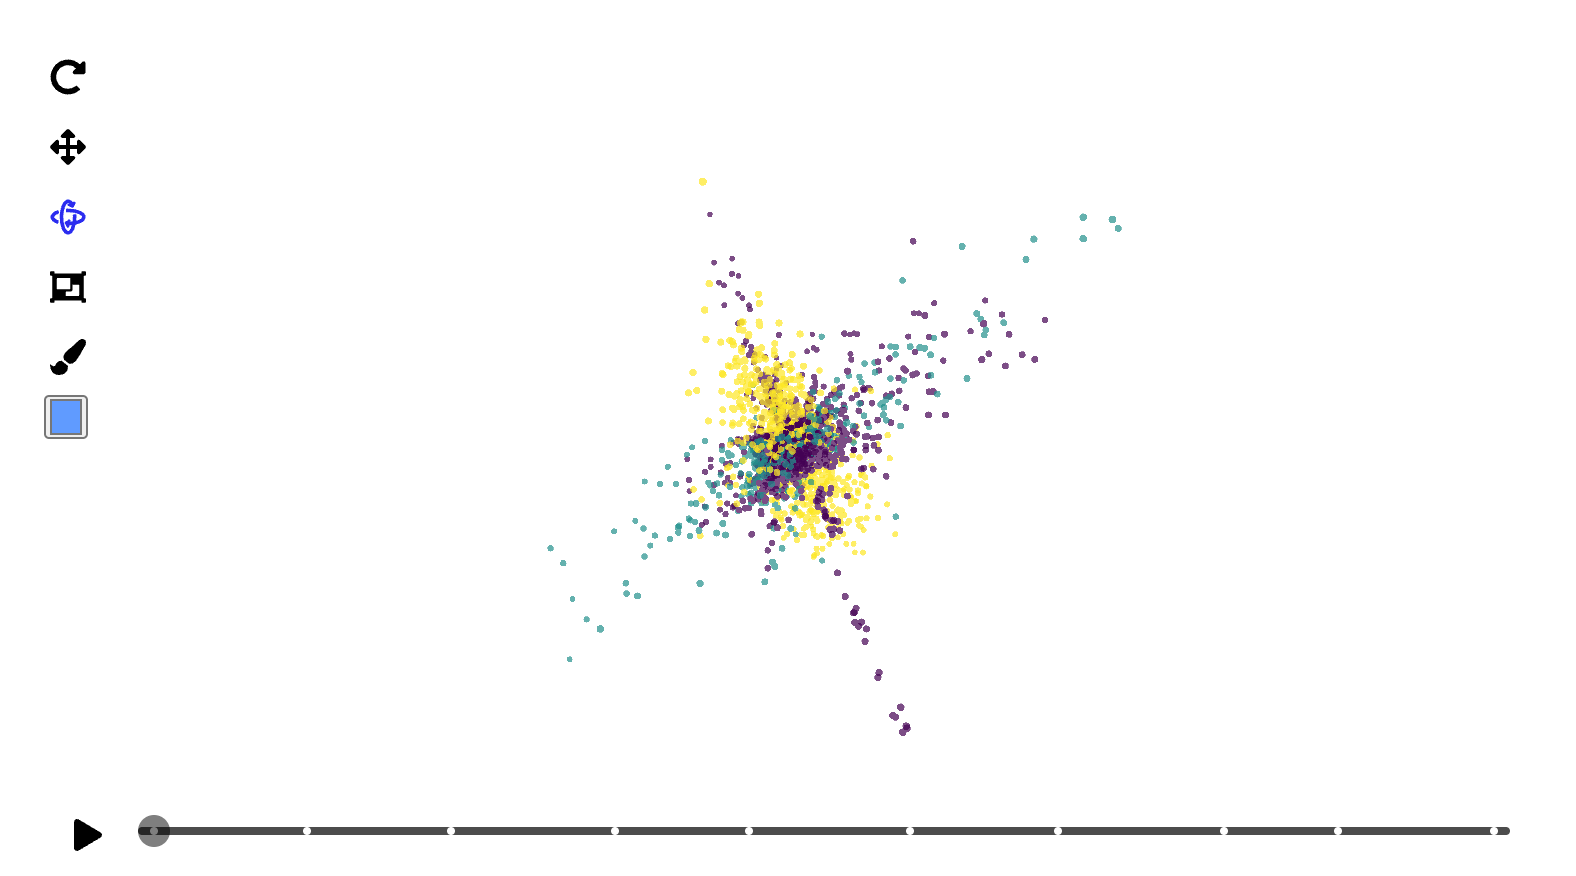
\includegraphics[width=\textwidth]{figures/implementation/pdfsense_scatter_3d} \caption{Initial frame of the scatterplot display generated by the `show\_scatter` display function. Controls are on the left, and an interactive timeline is on the bottom of the plot.}\label{fig:scatter-display-static}
\end{figure}

The output of \texttt{tour\_path()} becomes the input of \texttt{show\_*()}, forming a fluent pipeline. For the three display methods described above, the common parameters are:

\begin{itemize}
\tightlist
\item
  \texttt{palette}: the colour palette to use for the tour.
\item
  \texttt{center}: whether the data should be centred before displaying.
\item
  \texttt{axes}: whether to show axis / what the axis titles should be
\item
  \texttt{edges}: a two-column numeric matrix defining indices of points where line segments should be drawn between
\item
  \texttt{paused}: whether the animation should be initialised in a paused state.
\item
  \texttt{scale\_factor}: used to scale the points in or out so that they appear on a sensible range, similar to a zoom function. Defaults to the reciprocal of maximum distance from a point to the origin, so that the points fit inside a unit ball.
\end{itemize}

There are also parameters specific to each display method, such as \texttt{slice\_relative\_volume} for \texttt{show\_slice()}, and \texttt{gamma} and \texttt{R} for \texttt{show\_sage()}. These details will be described further in the Display Methods section.

\pagebreak

Putting all of this together, we have:

\begin{verbatim}
detour(pdf_df, tour_aes(
    projection = starts_with("PC"),
    colour = Type,
    label = ID
)) |>
    tour_path(grand_tour(3)) |>
    show_scatter()
\end{verbatim}

This chaining process allows us to construct the tour visualisation incrementally in a way that is intuitive and easy to follow. The user is able to inspect the result at each step in the chain, and it aligns well with the \emph{grammar of graphics} and \emph{tidy data} workflows. This makes \pkg{detourr} accessible to newcomers who may not have worked with tours previously.

\hypertarget{interactivity}{%
\subsection{Interactivity}\label{interactivity}}

Presently, several well-developed R packages allow the use of web technologies in R; \pkg{htmlwidgets} allows binding R code with HTML and JavaScript to create standalone widgets; \pkg{shiny} provides features for combining various elements in to interactive web applications powered by R; \CRANpkg{crosstalk} (Cheng and Sievert (2022)) enables linked selection and brushing between different HTML Widgets; and \CRANpkg{rmarkdown} (Allaire et al. (2022)) allows creating HTML documents with HTML Widgets embedded within. The use of web technologies such as JavaScript enable the resulting visuals to be portable and accessible, and enable the implementation of rich interactive features. In this section we will describe these interactive features and how they can be configured.

\hypertarget{label-aesthetics}{%
\subsubsection{Label aesthetics}\label{label-aesthetics}}

In the above example, labels are defined within the call to \texttt{tour\_aes()}, which contains all of the aesthetic mappings for the tour. The \texttt{label} aesthetic produces a tooltip which is shown whenever the mouse is hovered over the data point. By default, the text in the tooltip will have the format \texttt{column\_name:\ value}, with each specified column on a new line. If users want more control over what appears in the tooltip, one can use the \texttt{I()} function so that the values in the aesthetic column appear as-is. For example in \ref{fig:hover-tooltip}, the left plot specifies the label aesthetic as \texttt{label\ =\ c(InFit,\ Type,\ ID,\ pt,\ x,\ mu)} and the right is specifies the label as-is by using \texttt{label\ =\ I(ID)} in the call to \texttt{tour\_aes()}. When using the \texttt{I()} function for the label aesthetic, only one column can be specified at a time.

\begin{figure}
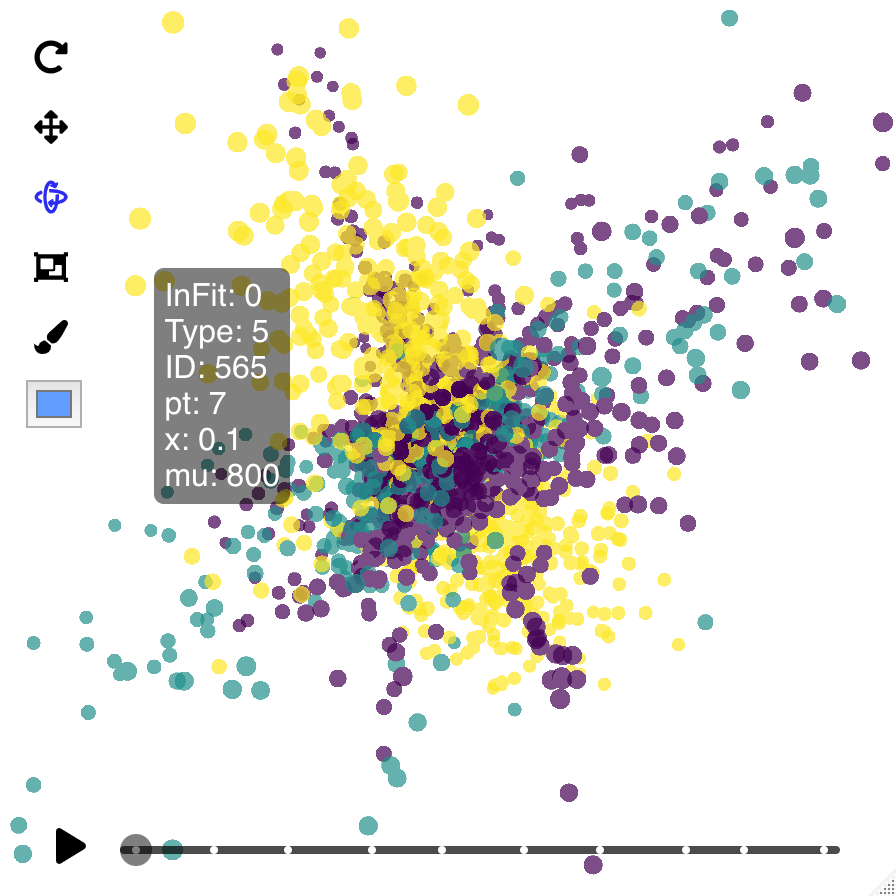
\includegraphics[width=0.5\linewidth]{figures/implementation/hover_tooltip} 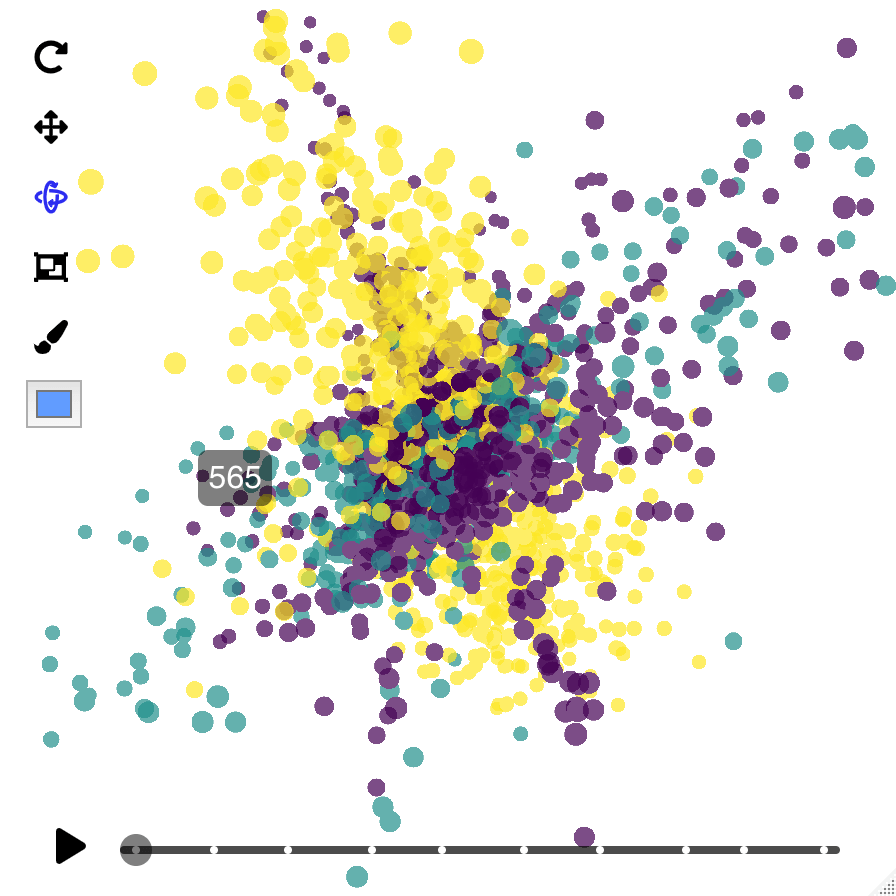
\includegraphics[width=0.5\linewidth]{figures/implementation/hover_tooltip_asis} \caption{(Left) Tooltip showing data from the 6 columns specified in the `label` aesthetic. Note that both the column names and values are present in the tooltip. (Right) The `ID` column is provided as-is to the label aesthetic via the `I()` function.}\label{fig:hover-tooltip}
\end{figure}

\hypertarget{controls}{%
\subsubsection{Controls}\label{controls}}

Table \ref{tab:pdf-controls} shows a breakdown of the controls found on the left side of the visual. Note that the icon for the currently selected control will be highlighted blue; otherwise it will be black. When the icons are hovered over in the \texttt{show\_scatter()} widget, alternative text will be shown.

\begin{table}

\caption{\label{tab:pdf-controls}An overview of the interactive controls available in the \pkg{detourr} displays}
\centering
\begin{tabular}[t]{>{\raggedright\arraybackslash}p{0.2\textwidth}>{\raggedright\arraybackslash}p{0.2\textwidth}>{\raggedright\arraybackslash}p{0.6\textwidth}}
\toprule
Control & Icon & Description\\
\midrule
Orbit & \raisebox{-\totalheight}{
\includegraphics[width=0.2\textwidth]{figures/implementation/orbit_control_button.png}} & When the `show\_scatter()` widget is generated, orbit controls will be enabled by default. This allows click and drag to rotate the visual, and scrolling/pinching to zoom. Note that orbit controls for the 2D variant work best if dragging from left to right, not up and down. Also note that the icon for the currently selected control will be highlighted blue; otherwise it will be black.\\
\midrule
Pan & \raisebox{-\totalheight}{
\includegraphics[width=0.2\textwidth]{figures/implementation/pan_button.png}} & The pan control also allows scrolling to zoom, and click and drag to pan.\\
\midrule
Box Selection & \raisebox{-\totalheight}{
\includegraphics[width=0.2\textwidth]{figures/implementation/select_button.png}} & The selection control allows for transitory box selection by brushing. Holding the `shift` key will allow for persistent selection, and points outside of the selection will be indicated by increased transparency. There is currently a limitation where only visible points can be selected. If a point is completely obscured by other points, it will not be selected.\\
\midrule
Brush & \raisebox{-\totalheight}{
\includegraphics[width=0.2\textwidth]{figures/implementation/brush.png}} & The brush button will apply the current colour to the selected points.\\
\midrule
Colour Selector & \raisebox{-\totalheight}{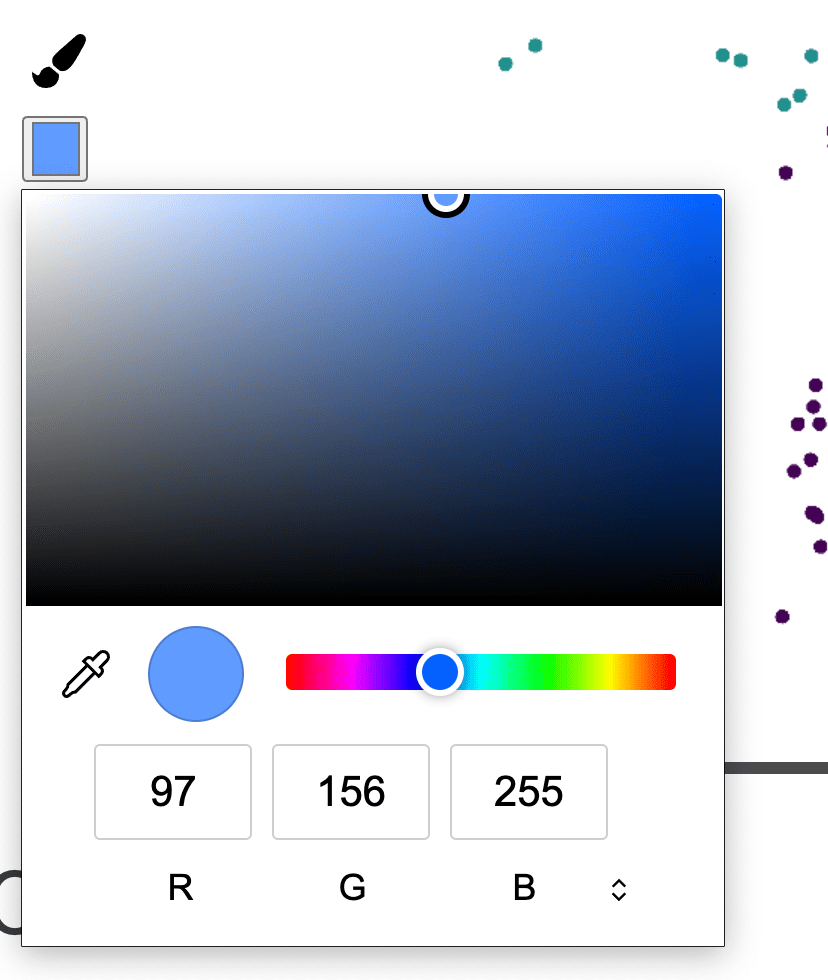
\includegraphics[width=0.2\textwidth]{figures/implementation/colour_selector.png}} & The colour selector will look slightly different depending on the browser being used. When the colour selection is changed, the selected points will be updated immediately.\\
\bottomrule
\end{tabular}
\end{table}

\begin{figure}
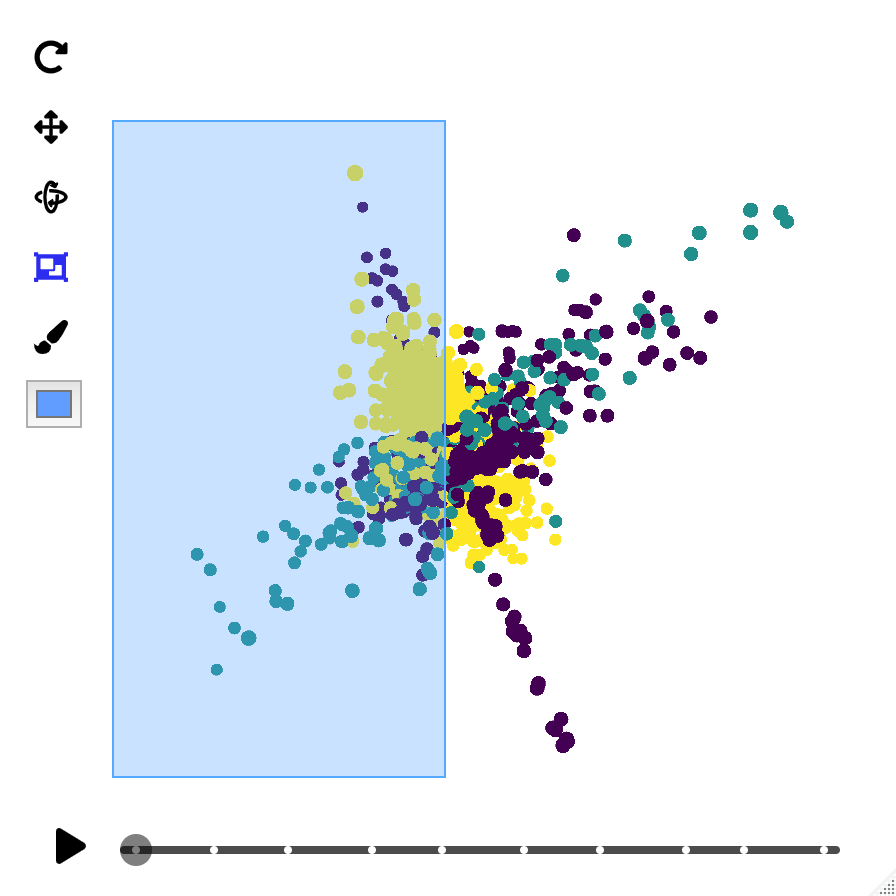
\includegraphics[width=0.49\linewidth]{figures/implementation/pdfsense-brushing-1} 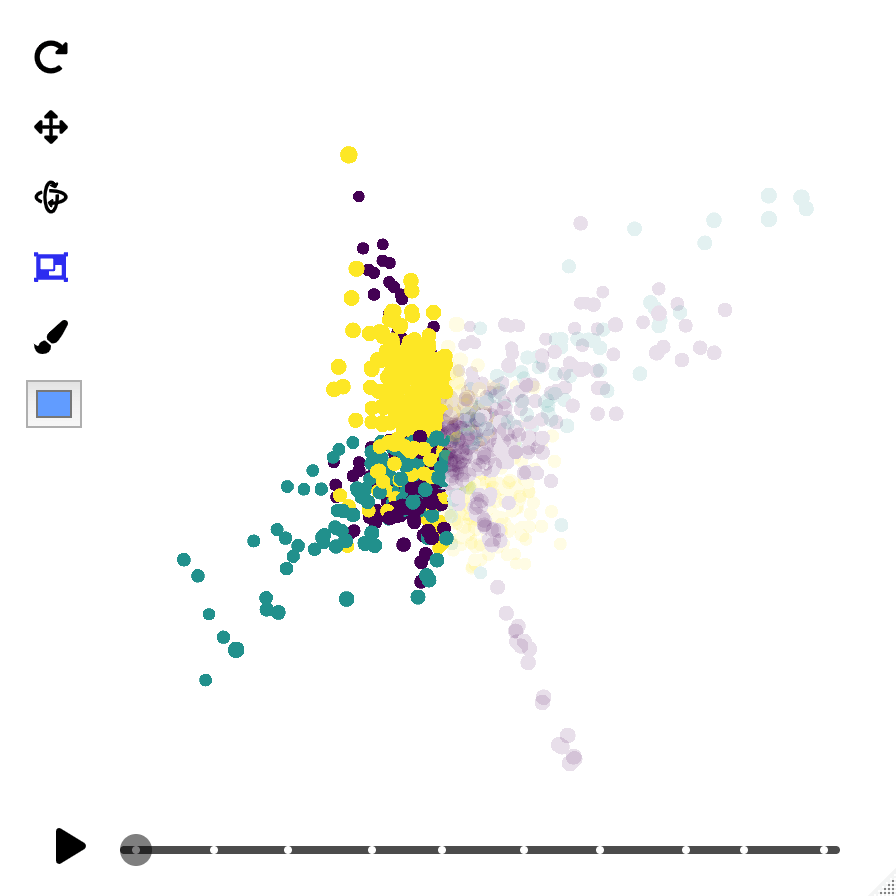
\includegraphics[width=0.49\linewidth]{figures/implementation/pdfsense-brushing-2} 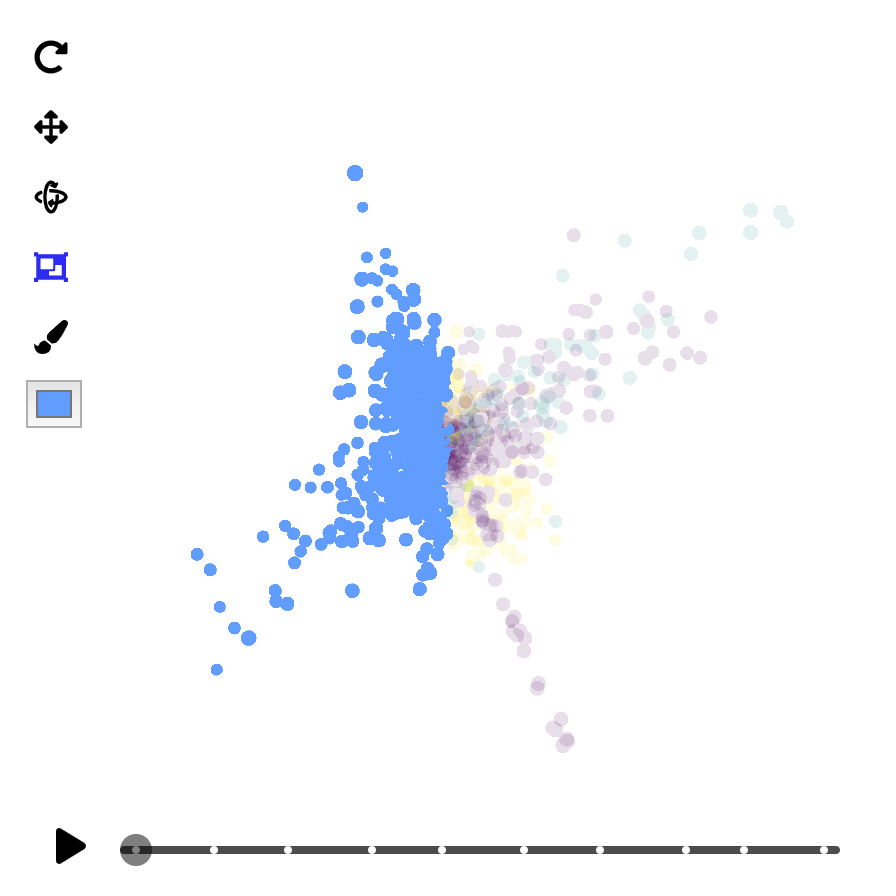
\includegraphics[width=0.49\linewidth]{figures/implementation/pdfsense-brushing-3} 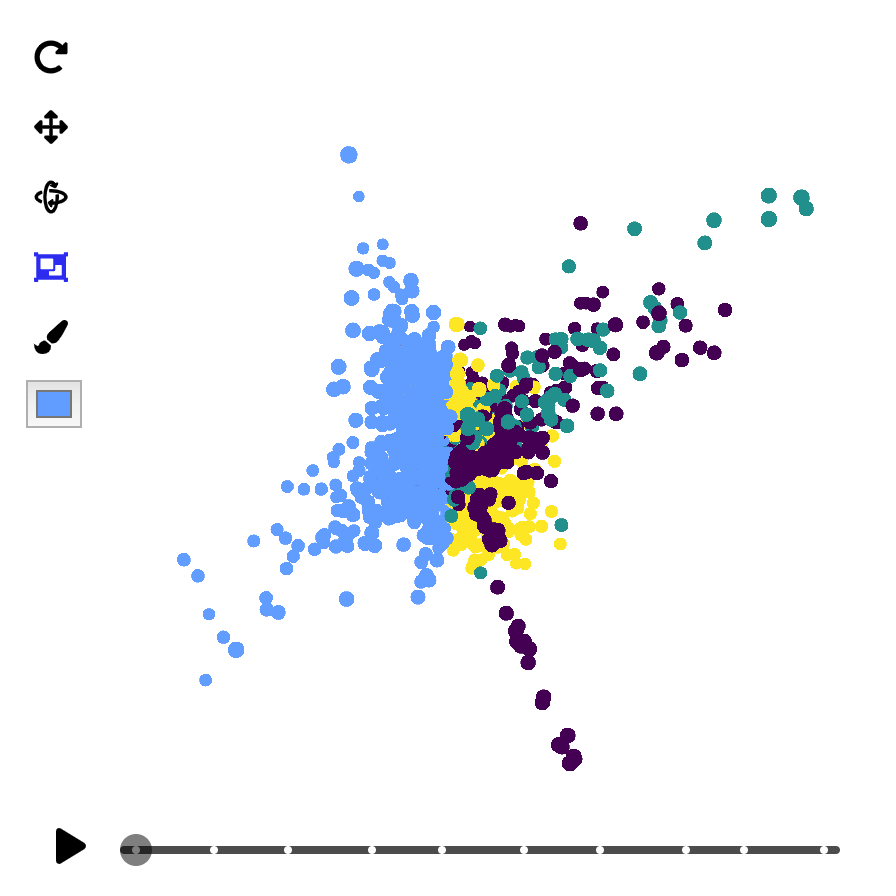
\includegraphics[width=0.49\linewidth]{figures/implementation/pdfsense-brushing-4} \caption{An illustration of the box selection and brush tool being used together.}\label{fig:brushing}
\end{figure}

\hypertarget{timeline-controls}{%
\subsubsection{Timeline controls}\label{timeline-controls}}

The timeline at the bottom of the widget controls play and pause, and allows for scrubbing to a specific point in the tour. The timeline can also be used to jump to a specific basis by clicking on any of the white basis markers, and hovering the mouse over the basis markers will display the index of that basis.

\hypertarget{linked-selection-and-filtering}{%
\subsubsection{Linked selection and filtering}\label{linked-selection-and-filtering}}

\pkg{detourr} supports linked selection and filtering by integrating with \pkg{crosstalk}. When a \pkg{crosstalk} \texttt{SharedData} object is provided to \texttt{detour()} in place of a data frame, selections made using the \emph{box selection} tool will be reflected in all linked visuals. Likewise, any selection or filtering applied to a linked visual will be reflected by \pkg{detourr}. Compatible widgets include \CRANpkg{plotly} (Sievert (2020)), \CRANpkg{leaflet} (Cheng, Karambelkar, and Xie (2022)), and \CRANpkg{DT} (Xie, Cheng, and Tan (2022)). An example of this is shown in the case study.

\hypertarget{web-technologies-for-performance}{%
\section{Web technologies for performance}\label{web-technologies-for-performance}}

One of the goals of this work is to improve upon the animation performance of existing tour displays. \pkg{detourr} uses several different web technologies to maximise performance so that smooth animations can be played with large data sets consisting of upwards of 100k data points. This performance also enables the animations to work with less powerful devices, making \pkg{detourr} accessible to a wider range of users.

The primary technology that allows for high-performance data visualisation is JavaScript itself. JavaScript engines in browsers such as Chrome and Firefox are highly optimised, leveraging methods such as Just-In-Time (JIT) compilation for improved runtime speed. However JavaScript is single-threaded, dynamically typed, and garbage collected, so despite these optimisations we can still run in to performance bottlenecks in some situations.

Figure \ref{fig:dataflow} shows a simplified overview of the data flow in \pkg{detourr} when creating and viewing a widget. On the left are the operations that are performed by R, which only occur once when the visual is first created and have a minimal performance impact. On the right are the main operations performed by JavaScript when the widget is displayed in a browser or IDE. Linear algebra and rendering operations need to run 30 times per second, so the technology decisions surrounding them have a big impact on performance. These technology decisions and are discussed in this chapter.

\begin{figure}
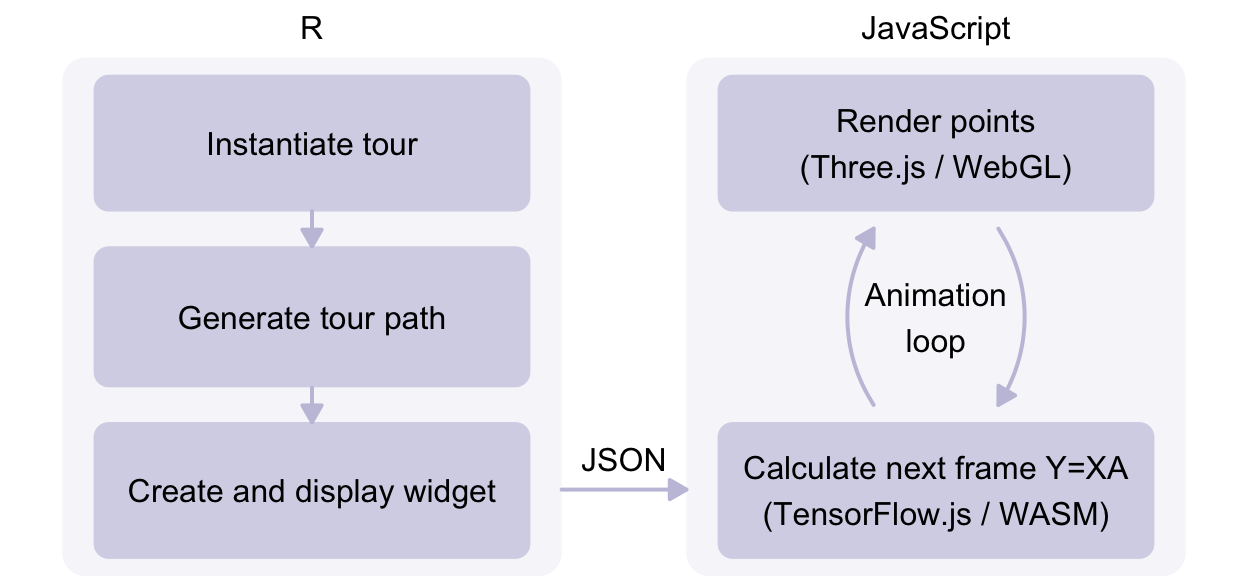
\includegraphics[width=\textwidth]{RJ-2023-052_files/figure-latex/dataflow-1} \caption{An overview of the data flow when creating a detourr visualisation. The full tour path is generated in R and then passed to JavaScript when the widget is created. The operations that occur in the animation loop in JavaScript are the most important to optimise.}\label{fig:dataflow}
\end{figure}

\hypertarget{linear-algebra-operations}{%
\subsection{Linear algebra operations}\label{linear-algebra-operations}}

The single-threaded nature of JavaScript makes matrix multiplication a performance bottleneck. At each animation frame, we must calculate the product \(\mathbf{XA}\) where \(\mathbf{X}\) is our data matrix and \(\mathbf{A}\) is our projection matrix. The slice tour generated by the \texttt{show\_slice()} display function requires an additional step of calculating the distance from each point to the projection plane which involves several more matrix operations.

To address this, \pkg{detourr} uses TensorFlow.js (Abadi et al. (2016)) as the main library for storing data and projection matrices and performing matrix operations. TensorFlow.js requires the user chose between one of three available backends:

\textbf{CPU} is a single-threaded JavaScript implementation which carries with it the limitations of JavaScript dynamic typing and garbage collection causing non-deterministic slow-downs at runtime.

\textbf{WebAssembly} (WASM) is a binary format that is used as a compilation target allowing code written in other languages like C, C++, and Rust to be run in the browser. This circumvents the dynamic typing and garbage collection limitations of JavaScript and allows near-native execution speed. The TensorFlow WASM backend uses the XNNPACK library from Google to accelerate matrix operations, which can run operations in parallel using threads and SIMD (Single Instruction Multiple Data).

\textbf{WebGL}: uses WebGL shaders to perform matrix operations on the GPU. According to the documentation, the performance benefit is primarily seen with large and complex deep learning models, so is unlikely to provide much benefit over the WebAssembly backend for our use case, and so is not investigated further in this section.

\hypertarget{performance-comparison}{%
\subsection{Performance comparison}\label{performance-comparison}}

To compare these backend options a simple performance profile was run in Microsoft Edge (Chromium) on a Macbook Pro 2019 (i7, 32Gb RAM). The implementations that were compared were:

\begin{itemize}
\tightlist
\item
  \emph{Hand Coded}: a manual JavaScript implementation coded using \texttt{for} loops, operating on nested arrays representing data and projection matrices.
\item
  \emph{TensorFlow CPU}: the vanilla single-threaded CPU backend for TensorFlow.js.
\item
  \emph{TensorFlow WASM}: the TensorFlow.js WASM backend.
\end{itemize}

These backends were compared across 3 datasets of different sizes and complexity, using a 2D Grand Tour:

\begin{itemize}
\tightlist
\item
  \emph{pdfsense}: The same data set used throughout this chapter; 2808 observations across 56 variables, taking the first 6 principal components for the tour.
\item
  \emph{mnist\_embeddings\_8d}: 8-dimensional embeddings of the MNIST dataset, with a total of 10k observations.
\item
  \emph{mnist\_embeddings\_32d}: 32-dimensional embeddings of the MNIST dataset, again with 10k observations.
\end{itemize}

\begin{figure}

{\centering 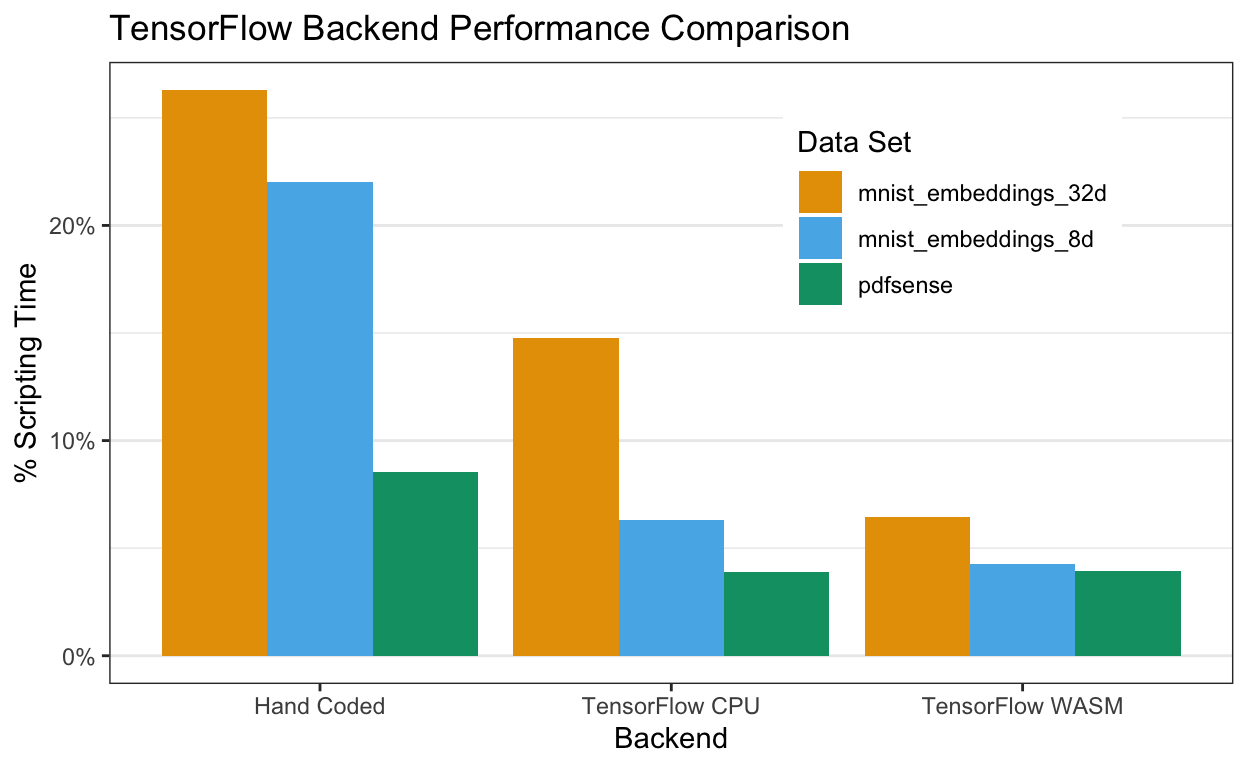
\includegraphics[width=0.75\linewidth]{RJ-2023-052_files/figure-latex/backend-comparison-1} 

}

\caption{Performance comparison across different data sets and backends. TensorFlow provides better performance than a hand-coded implementation across the board. For smaller datasets like pdfsense, there is little difference between CPU and WASM backends for TensorFlow.js, but for larger dataset WASM performs much better.}\label{fig:backend-comparison}
\end{figure}

Figure \ref{fig:backend-comparison} shows the performance of the three backends across the example datasets. TensorFlow provides better performance across the board when compared to the hand-coded implementation, but the difference between the CPU and WASM backends only becomes apparent with the larger MNIST embeddings datasets. Note that the metric \texttt{\%\ Scripting\ Time} is the time spent across \emph{all} JavaScript scripting for the visual, and not just the time spend on linear algebra operations. This is why we see such diminishing returns with the smaller \emph{pdfsense} dataset.

Another important comparison is the performance of the \texttt{show\_slice()} display function between these datasets. The slice tour uses additional matrix operations to calculate the distance from each point to the projection plane, so the benefit of WASM backend is even more apparent. This is shown in Figure \ref{fig:backend-comparison-slice}

\begin{figure}

{\centering 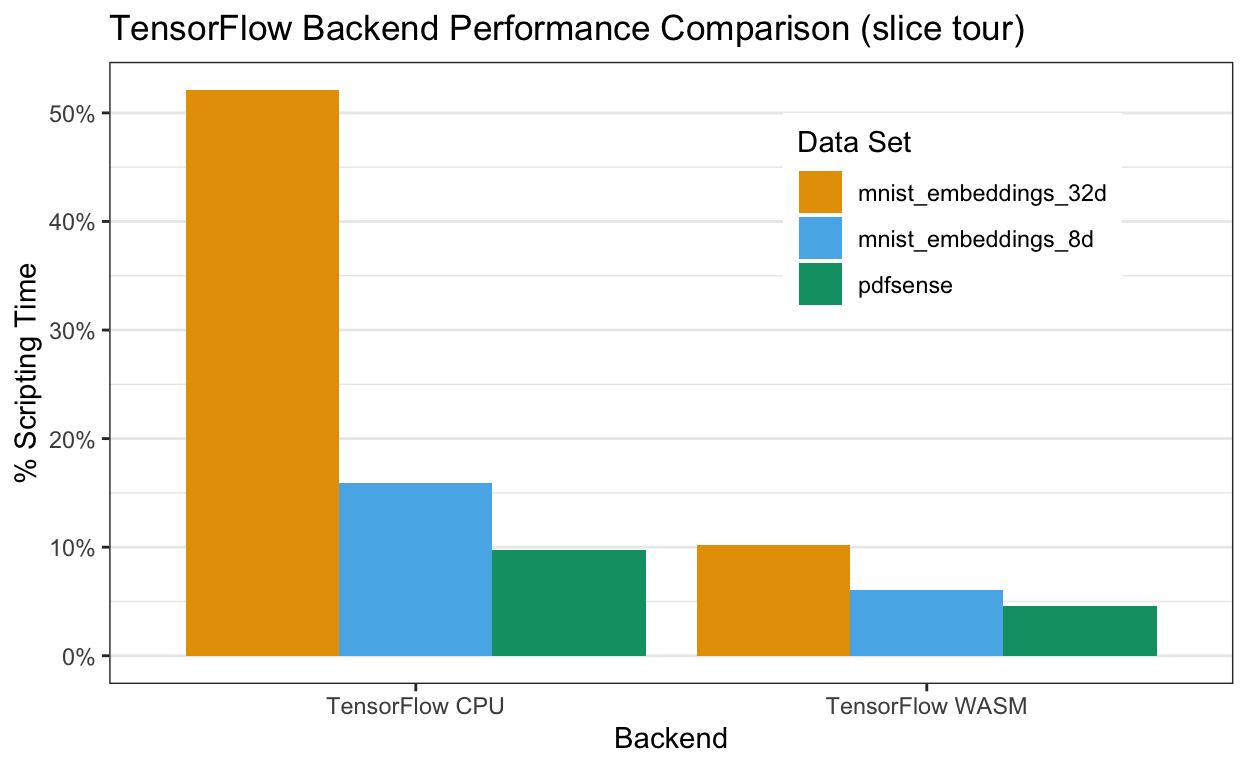
\includegraphics[width=0.75\linewidth]{RJ-2023-052_files/figure-latex/backend-comparison-slice-1} 

}

\caption{The additional matrix operations required by the slice tour display function make the performance benefit of the WASM backend much more apparent.}\label{fig:backend-comparison-slice}
\end{figure}

\hypertarget{rendering}{%
\subsection{Rendering}\label{rendering}}

When displaying data visuals using JavaScript in a browser, there are three main technologies that can be used:

\textbf{SVG} is commonly used for web-based visuals, including in software such as D3.js (Bostock, Ogievetsky, and Heer (2011)) with good support for interaction and animation. Kipp, Laa, and Cook (2019) uses D3.js with SVG for rendering tours, but describes performance issues when the number of points gets close to 2,000. This is because while SVG is suitable for drawing large and complex shapes, performance can degrade when rendering many individual shapes.

\textbf{HTML5 Canvas (2D)} uses a canvas element with a 2D rendering context and provides good performance, allowing many thousand data points to be used with smooth animation. This is the rendering method used by the \pkg{langevitour} package, and provides much better performance over SVG for this use case.

\textbf{HTML5 Canvas (WebGL)} uses the WebGL rendering context with GPU acceleration to achieve high performance, and is used by a range of browser-based 3D animations and games. This typically provides higher performance than using the 2D canvas rendering context.

\pkg{detourr} implements \textbf{HTML5 Canvas} with the \textbf{WebGL} rendering context using the Three.js (Cabello (2010)) library. This is the same library that powers the TensorFlow Embedding Projector (Smilkov et al. (2016)), and allows for flexible and performant 2D and 3D data visuals.

One downside of using HTML5 Canvas elements is that custom logic is needed to determine where the mouse pointer is relative to visual elements when interactions occur. This issue is resolved is by rendering the image twice; the first pass renders to the screen and the second renders to an invisible ``picking'' scene. The colours of the points in this picking scene correspond to the ID of the point that was rendered. When a mouse is hovered over a pixel or a set of pixels are selected, we simply check their colour in the picking scene to determine which point IDs relate to the event. Rendering the scene twice at each frame makes performance all the more important.

Despite this extra step, a naive performance benchmark of the rendering performance of \pkg{detourr} using the \texttt{mnist\_embeddings\_8d} data set at 30 FPS shows only 3\% of the time is devoted to rendering and painting points, which for our use case is negligible.

\hypertarget{display-methods-1}{%
\section{Display methods}\label{display-methods-1}}

There are three display functions implemented in the \pkg{detourr} package: \texttt{show\_scatter()}, \texttt{show\_sage()}, and \texttt{show\_slice()}. All three support 2D and 3D tour paths, and are based on the core \texttt{show\_scatter()} function. In this section, we will delve in to some of the implementation details of these functions and how the original and \emph{sage} display has been extended to three dimensions.

\hypertarget{scatter-display}{%
\subsection{Scatter display}\label{scatter-display}}

The scatter display forms the core of the three display methods, and contains all of the features and interactions described in previous sections. It is implemented in TypeScript using the Three.js library (Cabello (2010)) for rendering and TensorFlow.js (Abadi et al. (2016)) for linear algebra operations.

\hypertarget{slice-display}{%
\subsection{Slice display}\label{slice-display}}

The slice display is implemented in the \texttt{show\_slice()} function, and is based on the \emph{slice tour} described in Laa, Cook, and Valencia (2020). At each animation frame, the distance from each point to the projection plane is computed. Those points closer than some threshold \(h\) to the projection plane are highlighted, and those further away are greyed out. Slices offset from the origin are also supported.

Despite the slice tour itself being equivalent to that in \pkg{tourr}, the implementation has been modified for a simpler implementation. Laa, Cook, and Valencia (2020) calculates the distance as:

\begin{equation}
\tilde \nu_i^2 = ||\mathbf{x}_i^\prime||^2
\label{eq:nu}
\end{equation}

where

\begin{equation}
\mathbf{x}_i^\prime = \mathbf{x}_i - 
  (\mathbf{x}_i \cdot \mathbf{a}_1)\mathbf{a}_1 - 
  (\mathbf{x}_i \cdot \mathbf{a}_2)\mathbf{a}_2
\label{eq:xprime}
\end{equation}

and similar for the 3-dimensional case but with an additional term. With some rearranging, we can instead express this with the equivalent:

\begin{equation}
\tilde \nu^2 = (\mathbf{X} - \mathbf{XAA}^T)^2 \mathbf{1}_p
\label{eq:nu2}
\end{equation}

This requires fewer terms than the original, and is in a form that is more elegant to implement using TensorFlow.js. The implementation is also the same for both the 2D and 3D variants which keeps the code simple.

\hypertarget{offsetting-the-slice}{%
\subsubsection{Offsetting the slice}\label{offsetting-the-slice}}

Laa, Cook, and Valencia (2020) provides a generalisation of equations \eqref{eq:nu} and \eqref{eq:xprime} for a projection plane passing through an arbitrary anchor point \(\mathbf{c}\) as follows:

\begin{enumerate}
\def\labelenumi{\arabic{enumi}.}
\tightlist
\item
  Calculate \(\mathbf{x_i}^\prime\) as per equation \eqref{eq:xprime}
\item
  Calculate the component \(\mathbf{c}^\prime\) of \(\mathbf{c}\) orthogonal to the projection plane as:
  \[
  \mathbf{c}^\prime = \mathbf{c} - (\mathbf{c} \cdot \mathbf{a}_1)\mathbf{a}_1 - (\mathbf{c} \cdot \mathbf{a}_2)\mathbf{a}_2
  \]
\item
  Calculate \(\nu_i^2 = || \mathbf{x}_i^\prime - \mathbf{c}^\prime ||^2 = \mathbf{x}_i^{\prime 2} + \mathbf{c}^{\prime 2} - 2\mathbf{x}_i^\prime \cdot \mathbf{c}^\prime\) where the cross-term is expressed as:
  \[
  \mathbf{x}_i^\prime \cdot \mathbf{c}^\prime = \mathbf{x_i} \cdot \mathbf{c} - 
    (\mathbf{c} \cdot \mathbf{a}_1)(\mathbf{x}_i \cdot \mathbf{a}_1) -
    (\mathbf{c} \cdot \mathbf{a}_2)(\mathbf{x}_i \cdot \mathbf{a}_2)
  \]
\end{enumerate}

With this method there are many terms to calculate, and it was found it was difficult to implement and test. To circumvent this issue we instead take a different approach. Rather than offsetting the \textbf{projection plane} to pass through the point \(\mathbf{c}\) and then calculating the distances for each point, we instead offset the \textbf{data points} by \(\mathbf{c}\) in the opposite direction. This gives a distance calculation between points and projection plane that is equivalent to the original implementation but is much simpler to calculate. First we calculate the offset points \(\mathbf{X}^\prime\):

\begin{equation}
\mathbf{X}^\prime = \begin{bmatrix}
    \mathbf{x}_1 - \mathbf{c} \\
    \mathbf{x}_2 - \mathbf{c} \\
    \vdots \\
    \mathbf{x}_n - \mathbf{c}
    \end{bmatrix}
\label{eq:xprime2}
\end{equation}

And then calculate the distances to the projection plane similar to equation \eqref{eq:nu2}:

\begin{equation}
\tilde \nu^2 = (\mathbf{X}^\prime - \mathbf{X}^\prime \mathbf{AA}^T)^2 \mathbf{1}_p
\label{eq:nu3}
\end{equation}

Figure \ref{fig:slice-sphere} shows a slice tour implemented using equations \eqref{eq:xprime2} and \eqref{eq:nu3} with an anchor of \((1, 0, 0)\). Initially \(v_1\) is almost parallel to the projection plane, and so the slice runs close to the origin and only the points near the outside of the hollow sphere are highlighted. As the tour progresses, \(v_1\) becomes nearly orthogonal to the projection plane, and so the slice runs close to the edge of the sphere and only a small number of points near the centre of the visual are highlighted.

\begin{figure}

{\centering 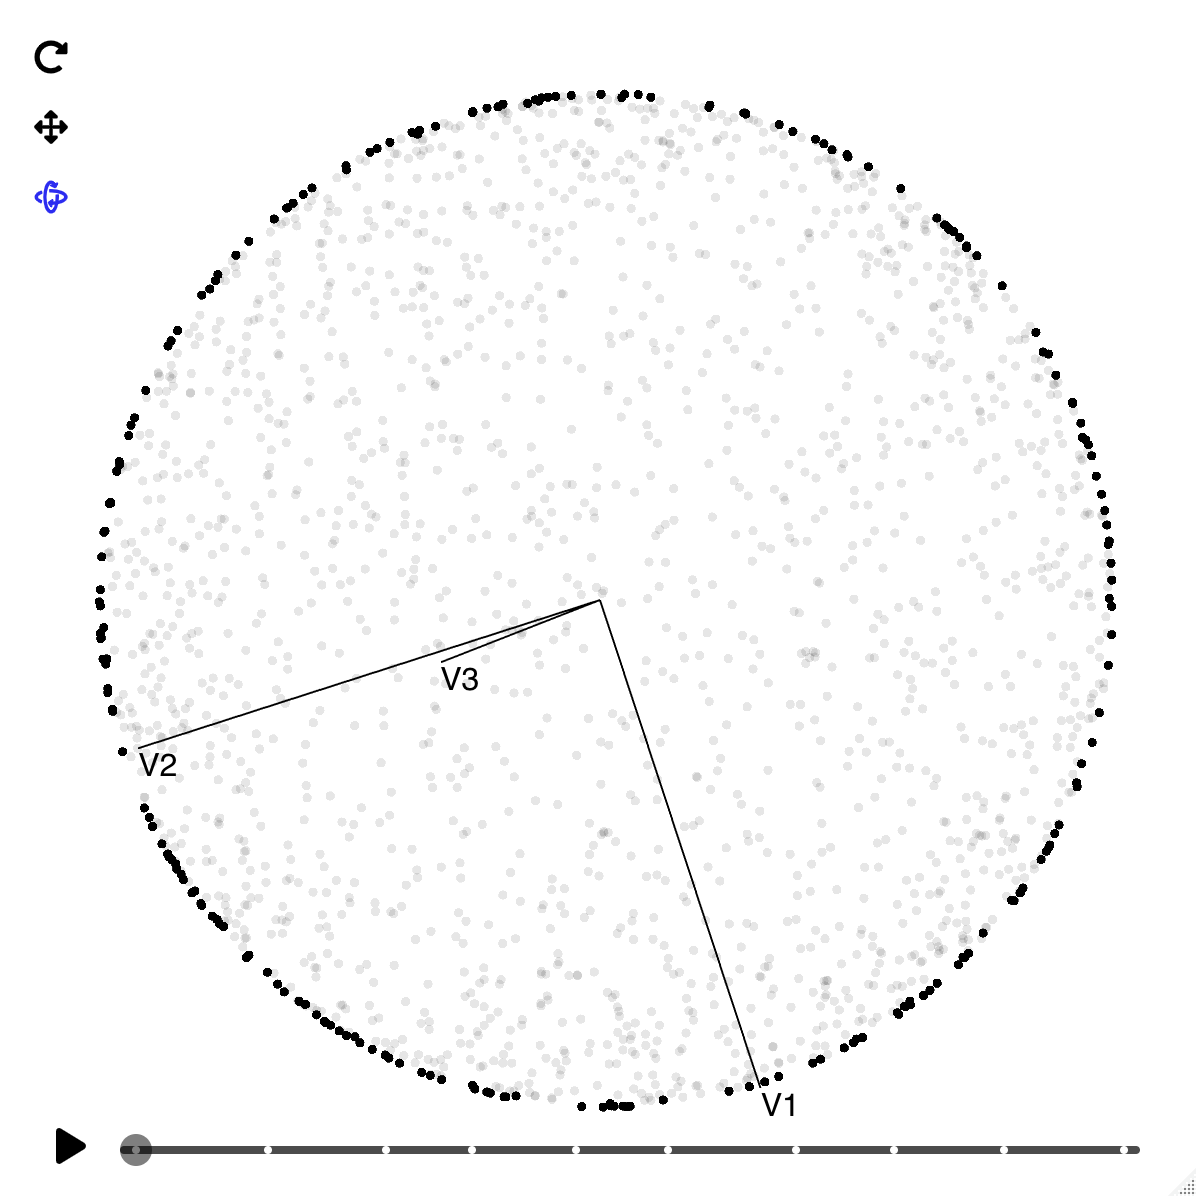
\includegraphics[width=0.32\linewidth]{figures/display_methods/slice_sphere_1} 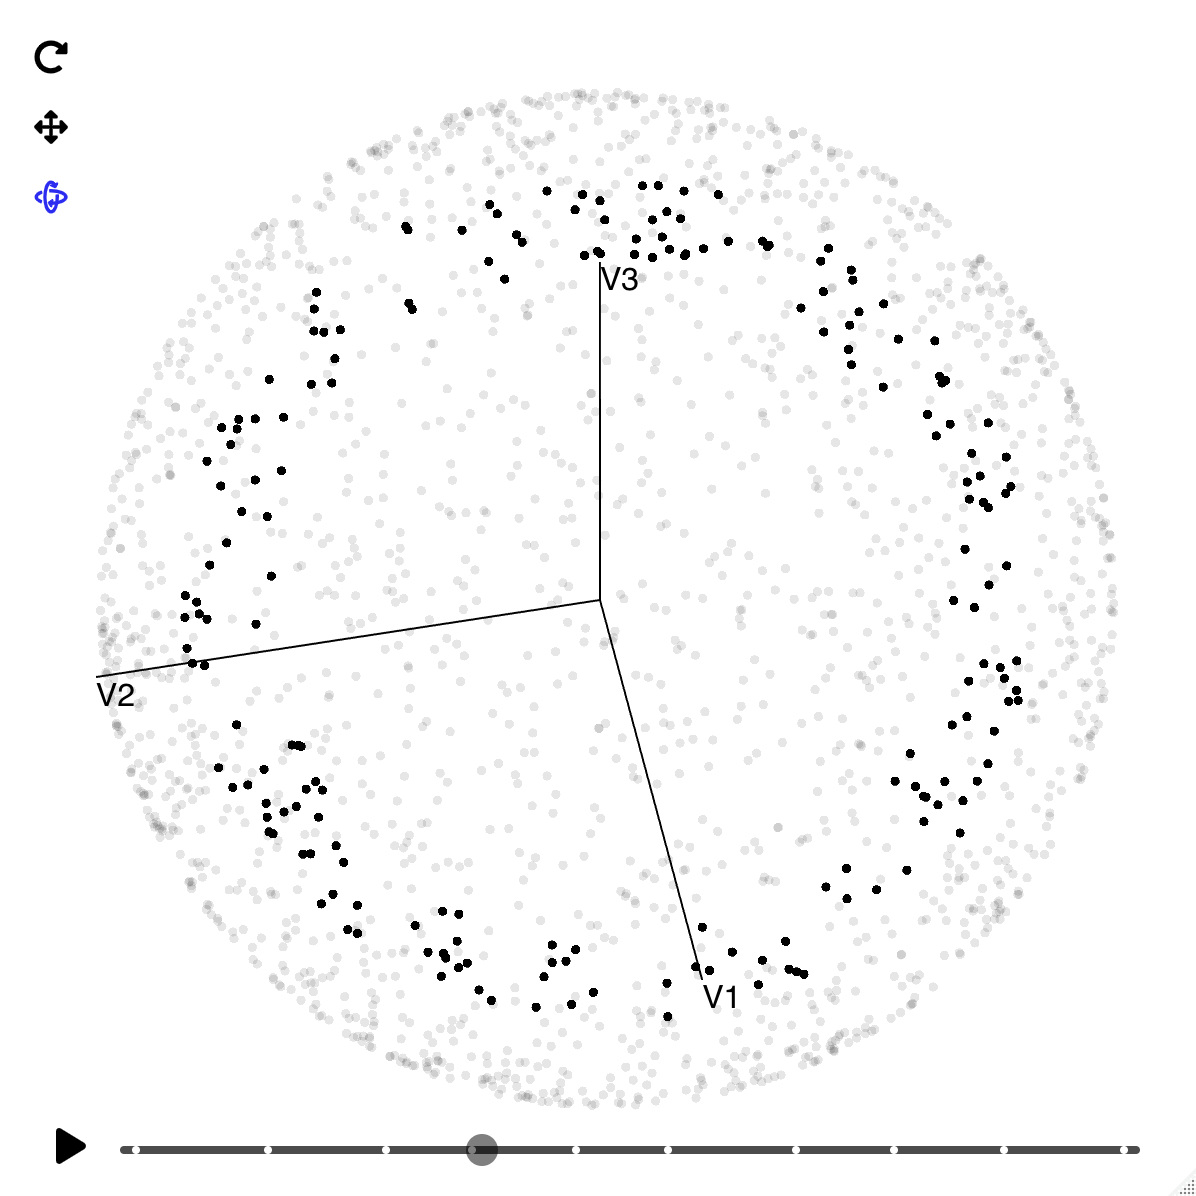
\includegraphics[width=0.32\linewidth]{figures/display_methods/slice_sphere_2} 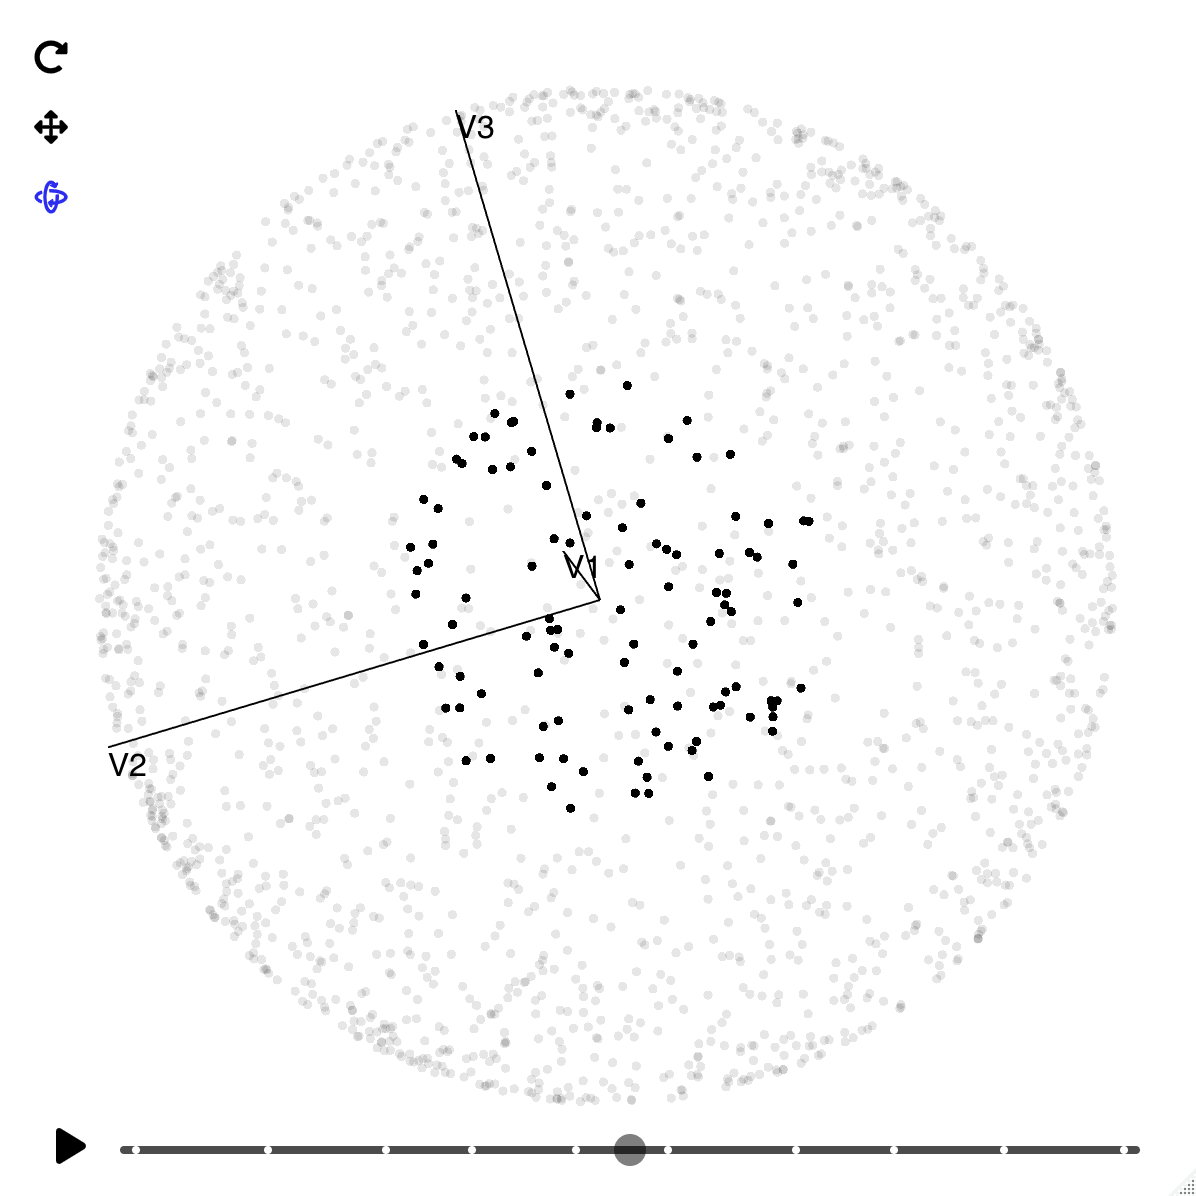
\includegraphics[width=0.32\linewidth]{figures/display_methods/slice_sphere_3} 

}

\caption{Selected frames of a 2D slice tour of a hollow unit sphere. The anchor for the slice is set to (1, 0, 0). Initially the slice is near the origin, but moves closer to the edge of the sphere as v1 rotates to be near orthogonal to the projection plane.}\label{fig:slice-sphere}
\end{figure}

\hypertarget{sage-display}{%
\subsection{Sage display}\label{sage-display}}

As the dimension of data increases, the volume of space that contains the data increases exponentially. One effect of this is that points tend to sit close to the edge of the space, with few points near the center. Hastie et al. (2001) gives a good illustration of this, where if we have \(N\) uniformly distributed points in a unit ball of dimension \(p\) centred at the origin, the median distance from the origin to the closest point is given by the equation

\begin{equation}
d(p, N) = \left( 1- \frac{1}{2}^\frac{1}{N}\right)^\frac{1}{p}
\end{equation}

Counter-intuitively, when we project data from a high-dimensional space to low-dimensions, we see the opposite effect where points tend to crowd towards the center of the projected space. Laa, Cook, and Lee (2021) describes a method for correcting this distortion so that points are less crowded towards the center. It does this by ensuring the relative volume at a given radius \(r\) in the original space is preserved in the projected space. The relative volume for a 2-dimensional projection is given by the equation

\begin{equation}
v_2(r; p, R) 
= \frac{V_{2D}(r; p, R)}{V(R,p)}
= 1 - \left(1-\left(\frac{r}{R}\right)^2\right)^\frac{p}{2}
\label{eq:radialcdf2d}
\end{equation}

where \(p\) is the dimension of our original data, \(R\) is the radius of the p-ball that contains our data, and \(r\) is the projected radius within \([0, R]\).

The formula for the corrected radius \(r_y^\prime\) is then given as

\begin{equation}
r_y^\prime = R \sqrt{1 - \left(1-\left(\frac{r}{R}\right)^2\right)^\frac{p}{2}}
\label{eq:radial2d}
\end{equation}

\pkg{detourr} uses a slight variation of equation \eqref{eq:radial2d} to calculate the corrected radius, which omits the multiplier of \(R\). This is because we always plot the data on the range \(r_y^\prime = [0, 1]\), so the multiplier is not needed:

\begin{equation}
r_y^\prime = \sqrt{1 - \left(1-\left(\frac{r}{R}\right)^2\right)^\frac{p}{2}}
\label{eq:radial2d2}
\end{equation}

The full implementation is as follows:

\begin{enumerate}
\def\labelenumi{\arabic{enumi}.}
\tightlist
\item
  Calculate the projected data \(\mathbf{Y} = \mathbf{XA}\), where \(\mathbf{X}\) has already been scaled.
\item
  Calculate the trimmed radius of the projected points \(r_y^\mathrm{trim} = min(r_y, R)\) and apply the radial transformation described in equation \eqref{eq:radial2d2} to get the corrected radius \(r_y^\prime\).
\item
  Scale the Euclidean point vectors by a factor of \(\frac{r_y^\prime}{r_y}\)
\end{enumerate}

This differs from the original implementation described in Laa, Cook, and Lee (2021) in that we don't convert the Euclidean vectors to polar form, and instead apply the scaling directly to the Euclidean vectors. This removal of the conversion step was primarily to improve performance.

\hypertarget{extension-to-3d}{%
\subsubsection{Extension to 3D}\label{extension-to-3d}}

Laa, Cook, and Lee (2021) provides the equation for the relative projected volume at radius \(r\) on to a two dimensional disk for the 2-dimensional sage display. In this paper, we extend and implement the scatter, sage, and slice displays in 3D, and to do this we needed to calculate the relative projected volume for the case of a 3-dimensional projection.

In the appendix we show that the relative projected volume for a \textbf{sphere} at radius \(r\) is given by:

\begin{equation}
  v_3(r; p, R) = \mathrm{BetaInc}\left(\left(\frac{r}{R}\right)^2, \frac{3}{2}, \frac{p-1}{2}\right) 
\end{equation}

Where \(\mathrm{BetaInc}(x, \alpha, \beta)\) is the regularised incomplete beta function. This is important because it represents the radial CDF of points projected to 3 dimensions, and suggests that the radial PDF of the projected points is \(\mathrm{Beta}\left(\frac{3}{2}, \frac{p-1}{2}\right)\) assuming the original data is a uniformly distributed ball of radius \(R\).

So for the three dimensional case, the full radial transformation for the sage tour is given by

\begin{equation}
r_y^\prime = \sqrt[3]{\mathrm{BetaInc}\left(\left(\frac{r}{R}\right)^2, \frac{3}{2}, \frac{p-1}{2}\right)}
\label{eq:radial3}
\end{equation}

We also show that this generalises to any projection from \(p\) to \(d\) dimensions with \(p>d\) with the equation:

\begin{equation}
v(r; p, R, d) = \mathrm{BetaInc}\left(\left(\frac{r}{R}\right)^2, \frac{d}{2}, \frac{p-d}{2}+1\right)
\label{eq:radiald}
\end{equation}

This also suggests that equation \eqref{eq:radialcdf2d} is a special case of equation \eqref{eq:radiald}.

The 3D sage tour is currently implemented in the \texttt{show\_sage()} function, and like the scatter and slice displays the correct variant is chosen automatically based on the dimension of the provided tour path. However, this is not implemented for \(d>3\) as we don't yet have a display method that can handle higher-dimensional projections. This will be implemented as an extension of a Parallel Coordinates Plot (PCP) or Andrew's plot in future.

An example of the 3D sage tour is shown in Figure \ref{fig:sage-sphere}.

\begin{figure}

{\centering 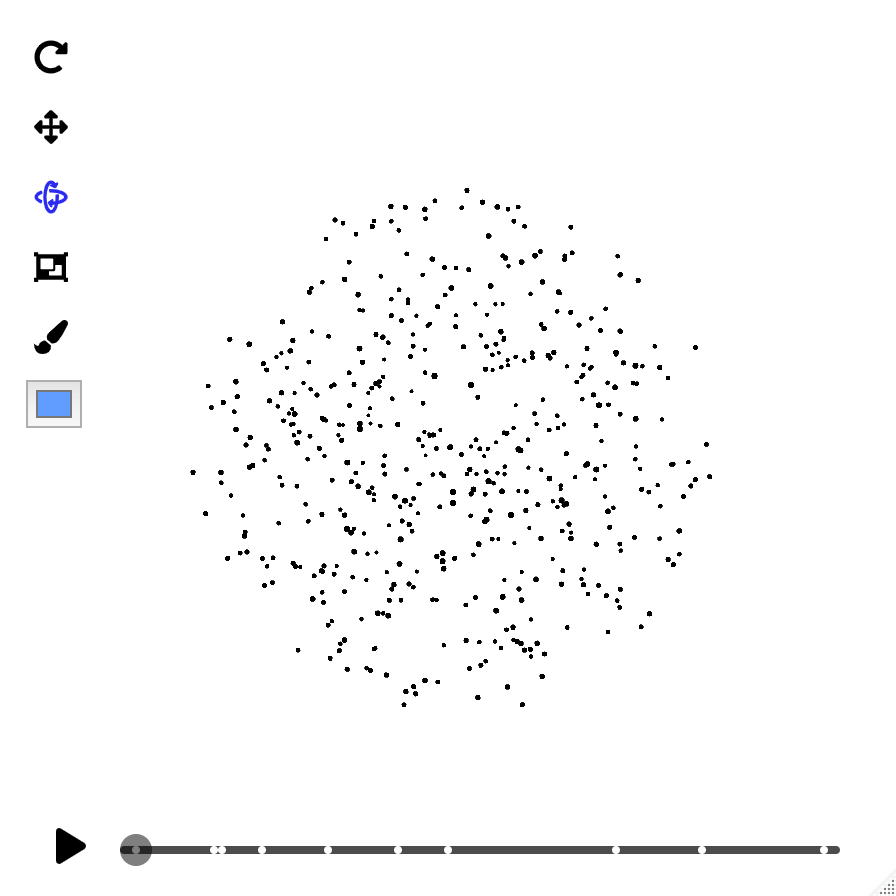
\includegraphics[width=0.32\linewidth]{figures/display_methods/scatter_sphere_3} 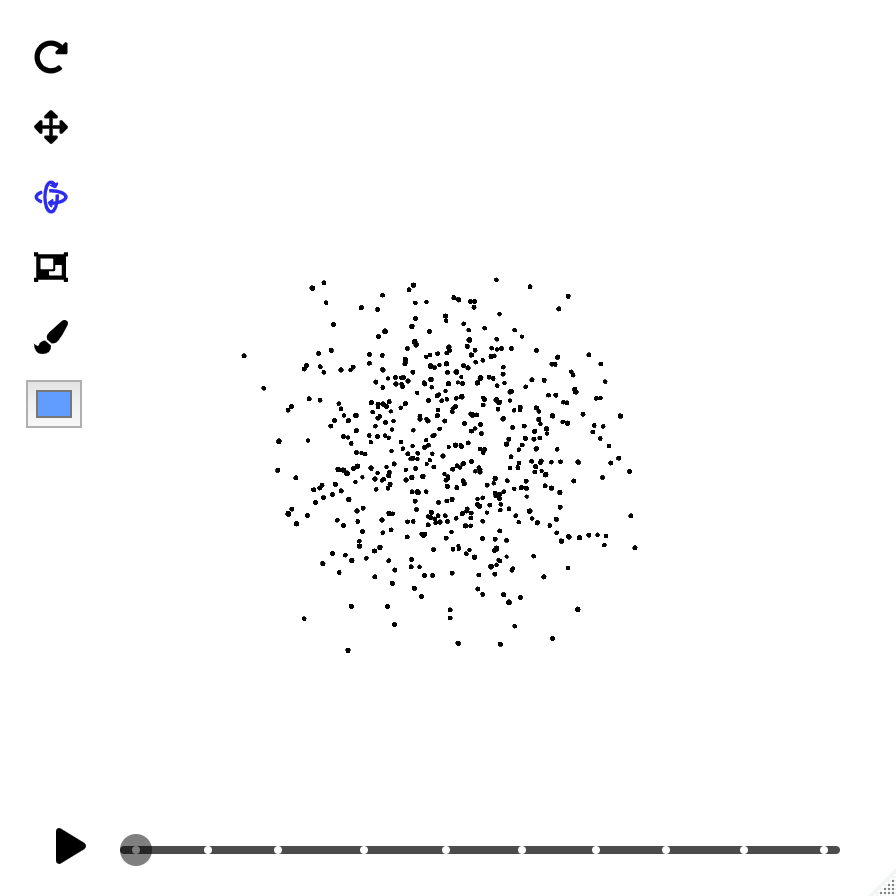
\includegraphics[width=0.32\linewidth]{figures/display_methods/scatter_sphere_10} 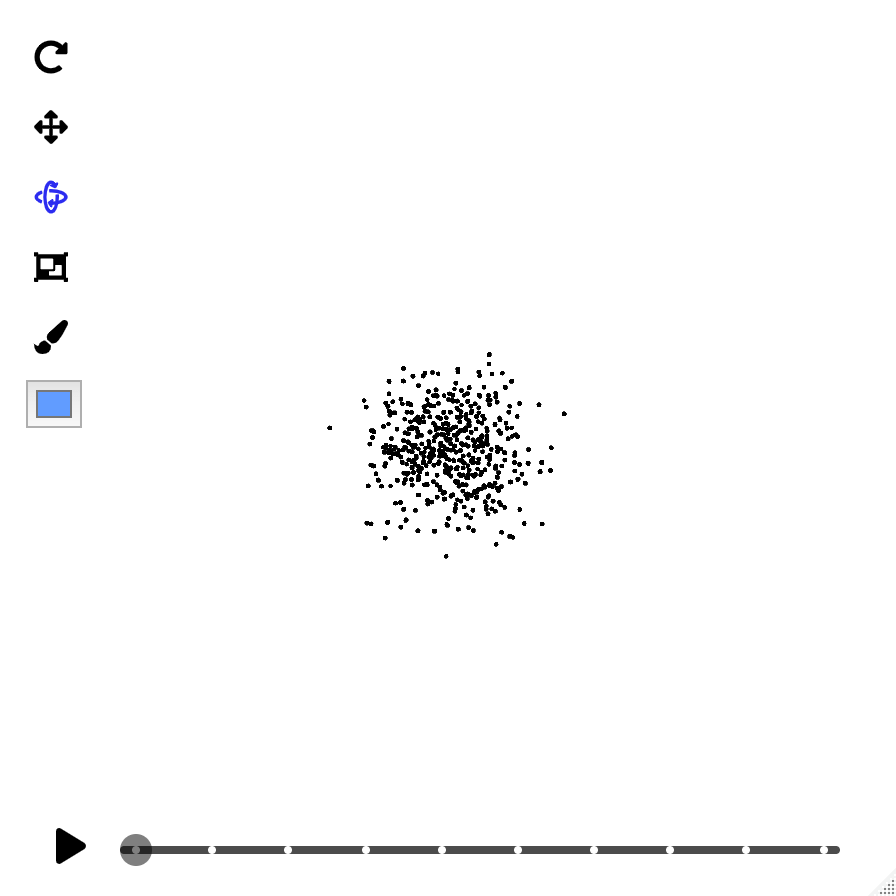
\includegraphics[width=0.32\linewidth]{figures/display_methods/scatter_sphere_50} 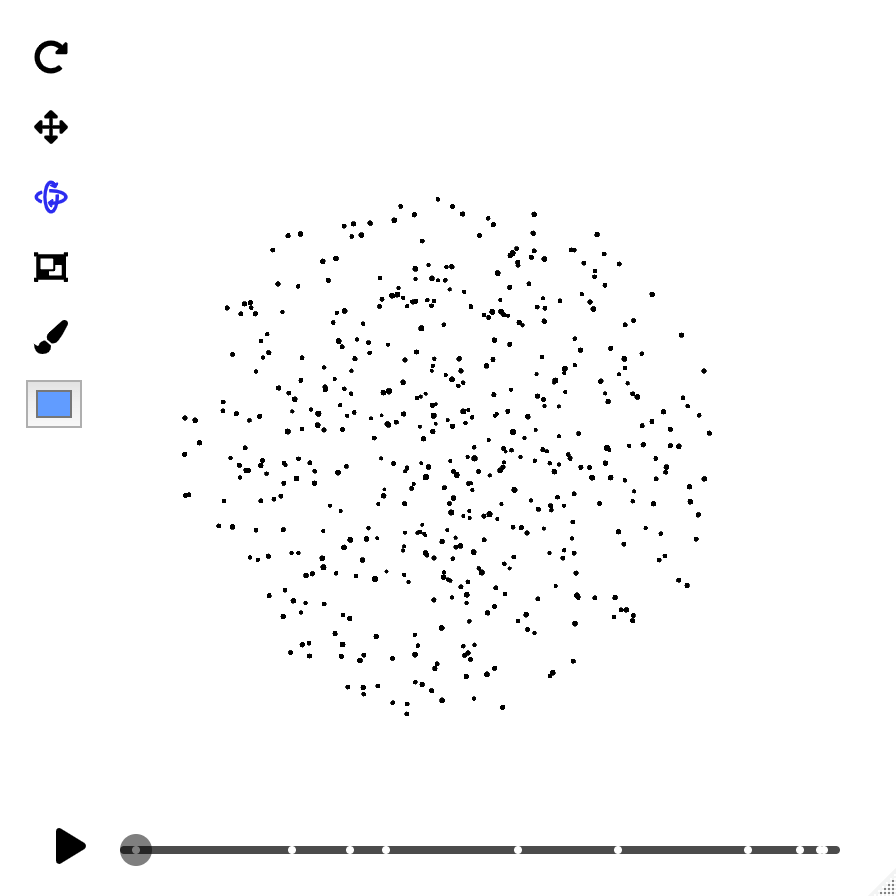
\includegraphics[width=0.32\linewidth]{figures/display_methods/sage_sphere_3} 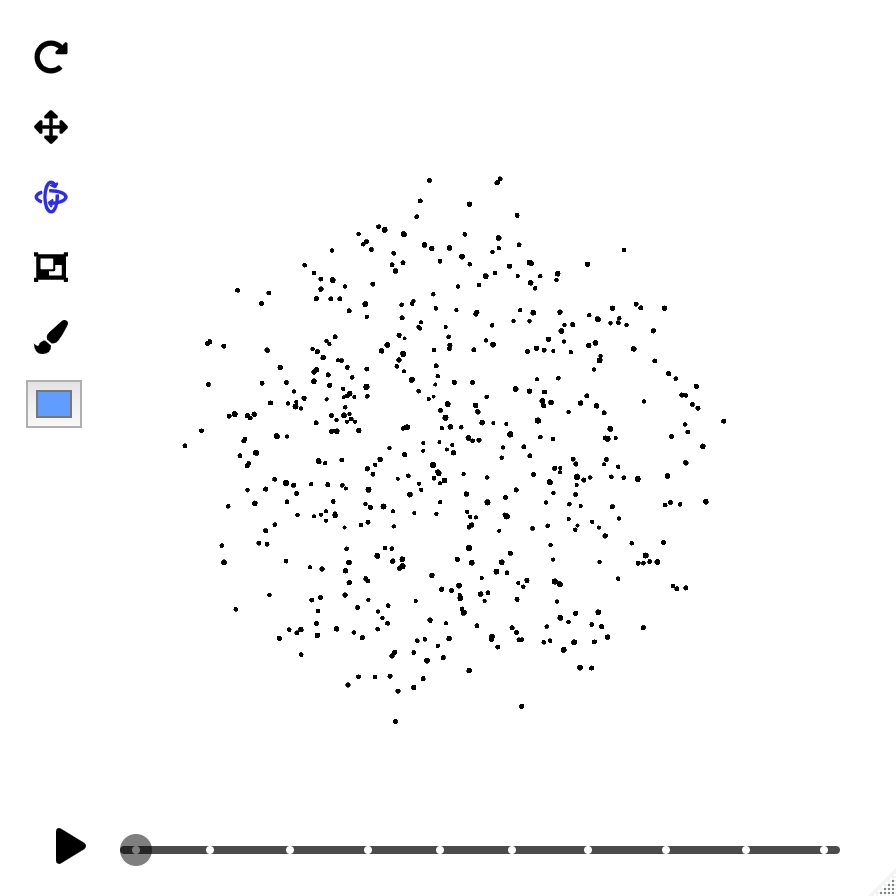
\includegraphics[width=0.32\linewidth]{figures/display_methods/sage_sphere_10} 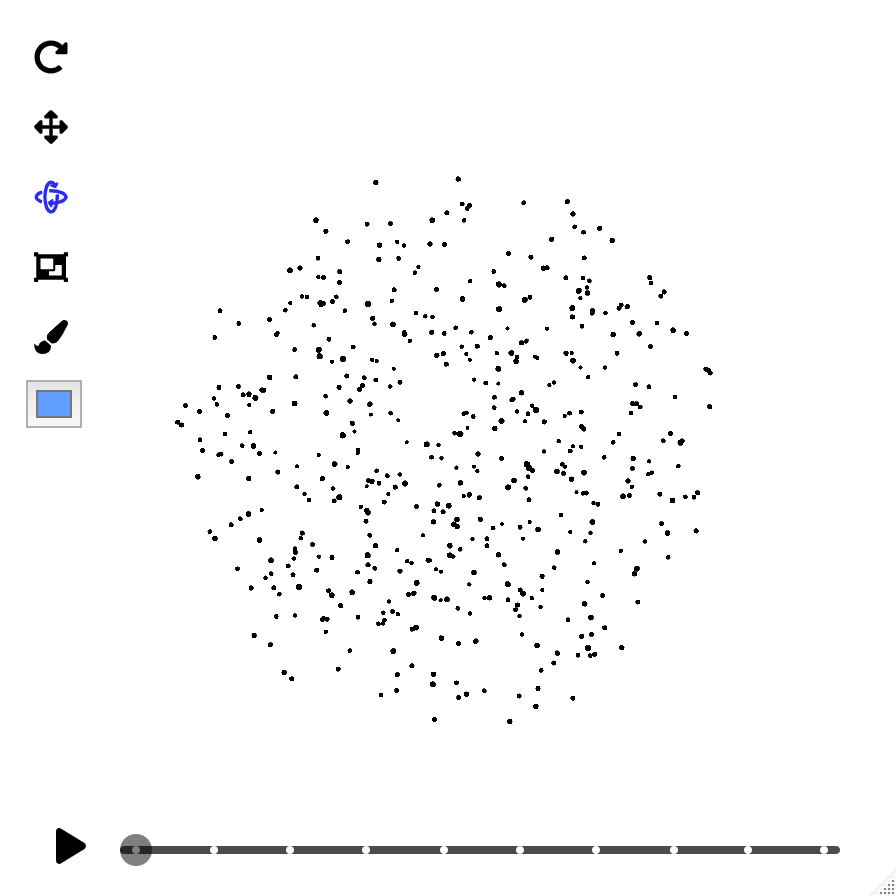
\includegraphics[width=0.32\linewidth]{figures/display_methods/sage_sphere_50} 

}

\caption{(Top) Initial frames of a 3D scatter tour of a 3, 10, and 50 dimensional ball respectively from left to right. (Bottom) Selected frames of a 3D sage tour of similar 3, 10, and 50 dimensional balls. As the dimensionality increases, the standard scatter display crowds the points near the center, whereas the sage display shows a consistent radial distribution of points. All screenshots are at the same zoom level.}\label{fig:sage-sphere}
\end{figure}

\hypertarget{case-study-mnist-embeddings}{%
\section{Case study --- MNIST embeddings}\label{case-study-mnist-embeddings}}

A common task when analysing wide or sparse data sets is to generate embeddings; finding a lower dimensional representation of high dimensional data, placing similar objects close together and dissimilar objects far apart in the embedding space. This is especially useful when dealing with text or image data.

An example of this is the algorithm used for facial recognition in FaceNet (Schroff, Kalenichenko, and Philbin (2015)). A neural network is trained which maps a vector representation of images of faces to a lower dimensional space. The network minimises the distance between examples of the same class and maximises distances between examples from different classes in the output space. The result is that the euclidean distance between faces can be used as a metric for face similarity, so an unknown face can be classified as belonging to a specific individual if the distance between the unknown face and one or more known faces is small.

The datasets \texttt{mnist\_embeddings\_8d} and \texttt{mnist\_embeddings\_32d} in the \pkg{detourr} package are embeddings trained using a similar algorithm to FaceNet but using the MNIST (LeCun (1998)) handwritten digits dataset. The training set consists of 60,000 28x28 pixel training images and in the following examples we visualise the test set containing 10,000 examples.

\hypertarget{scatterplot-display}{%
\subsection{Scatterplot display}\label{scatterplot-display}}

\begin{figure}

{\centering 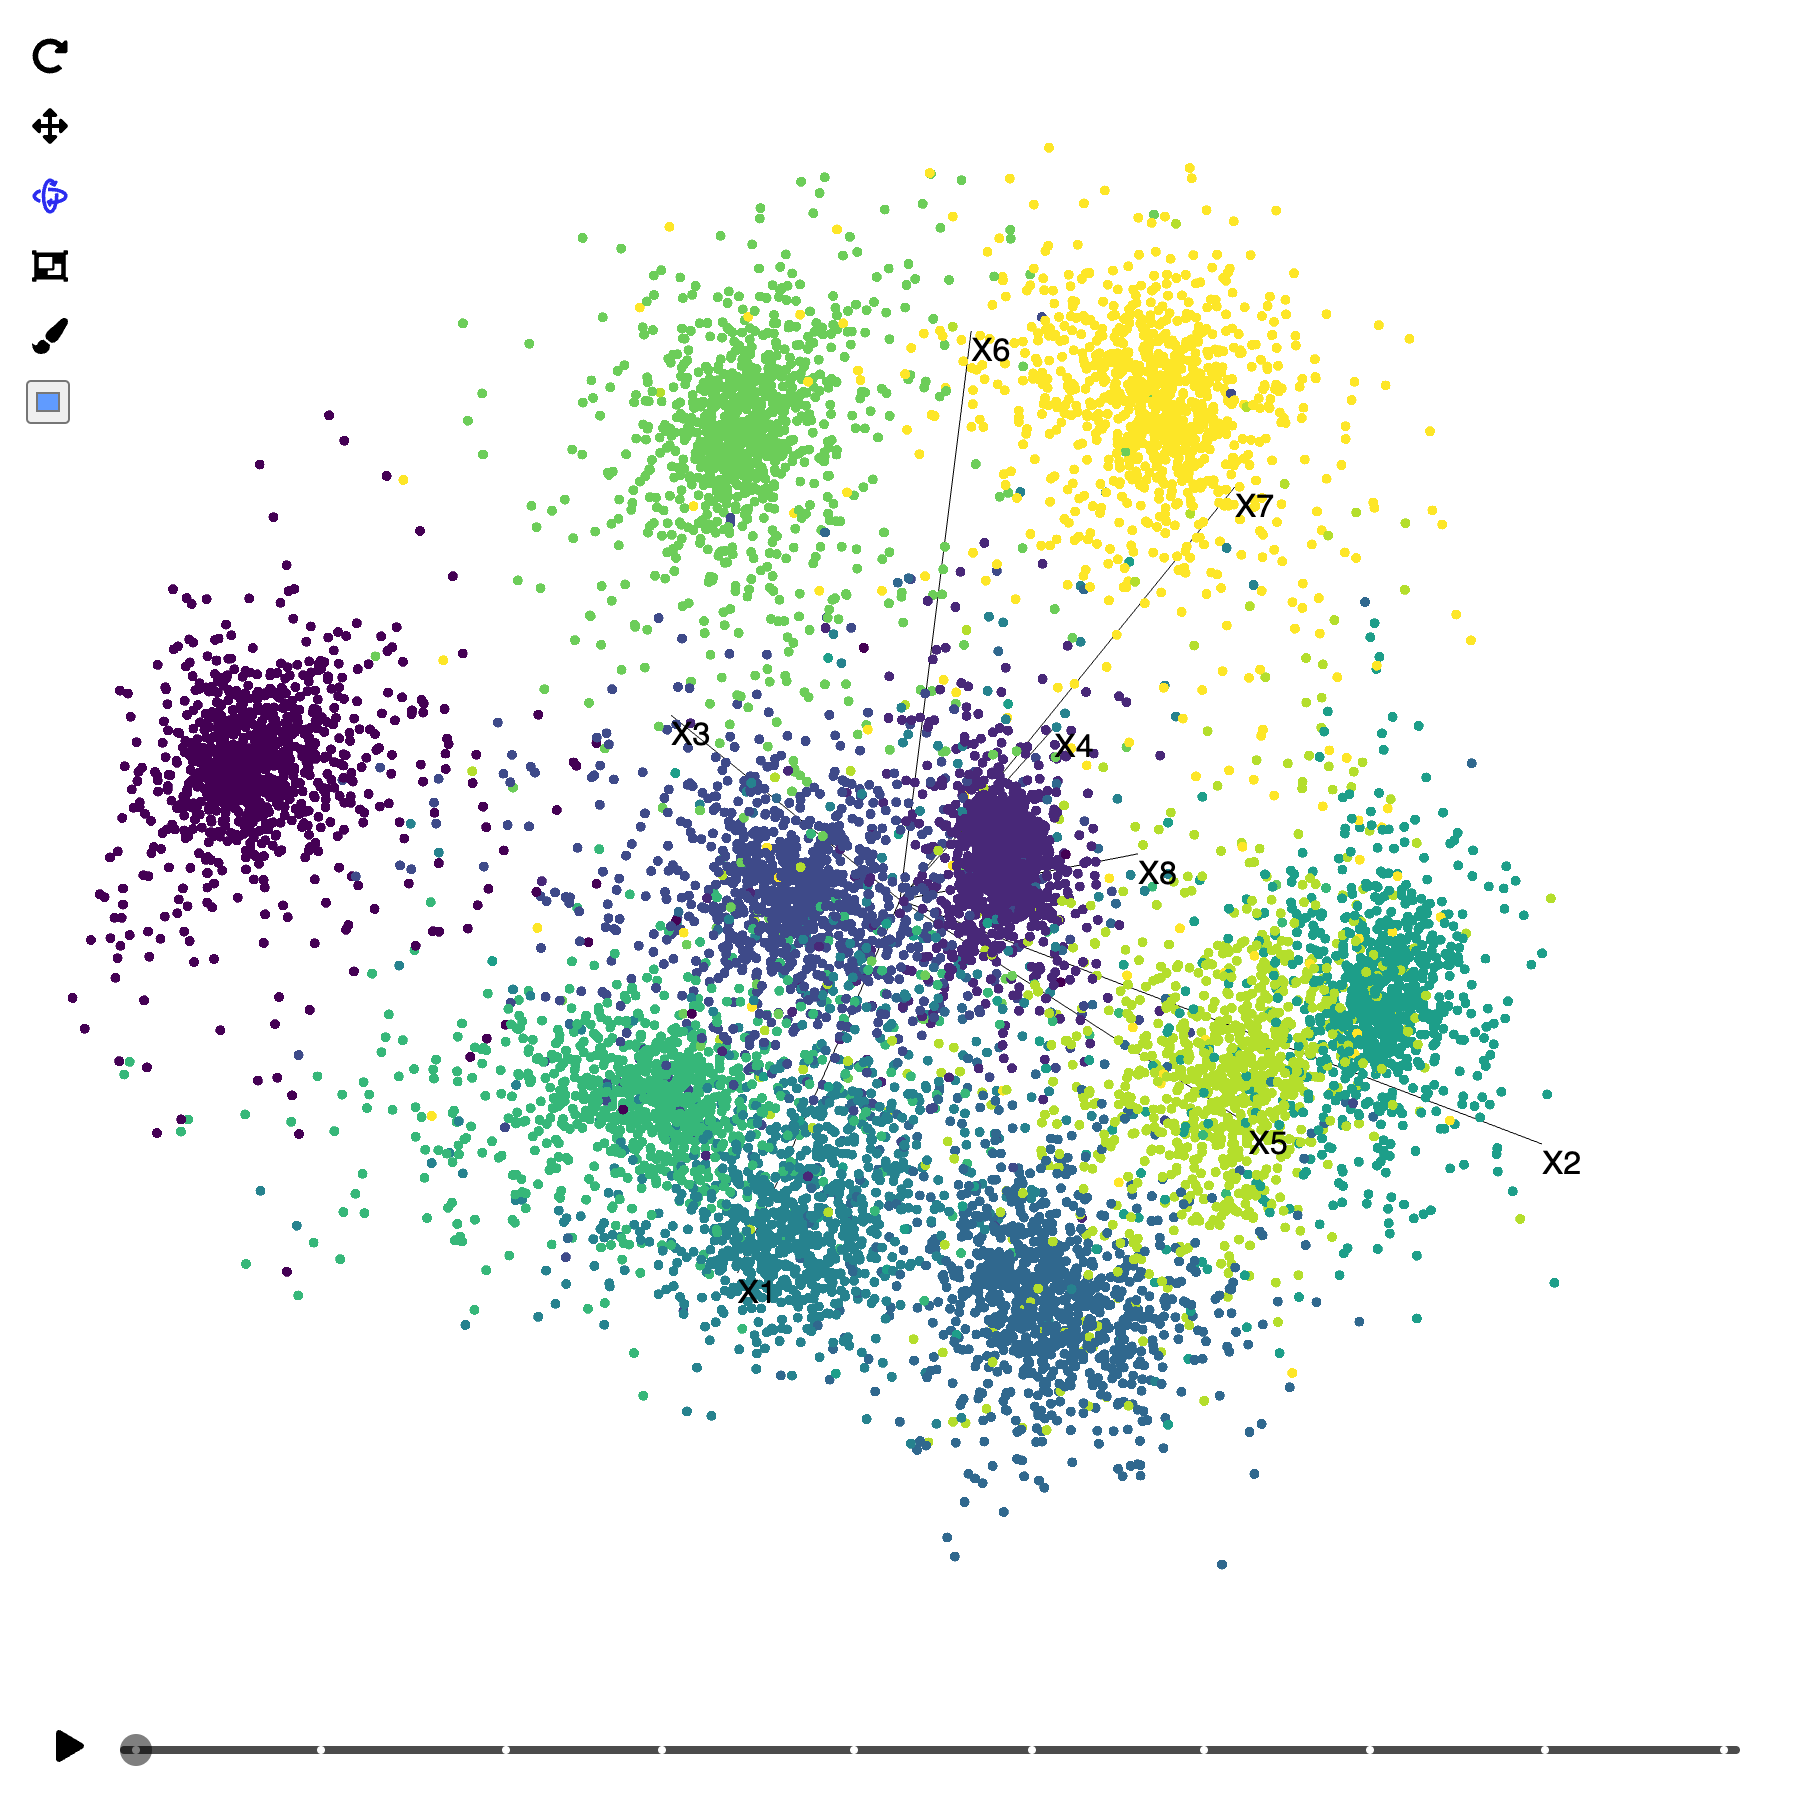
\includegraphics[width=0.49\linewidth]{figures/mnist/mnist-8d-scatter-1} 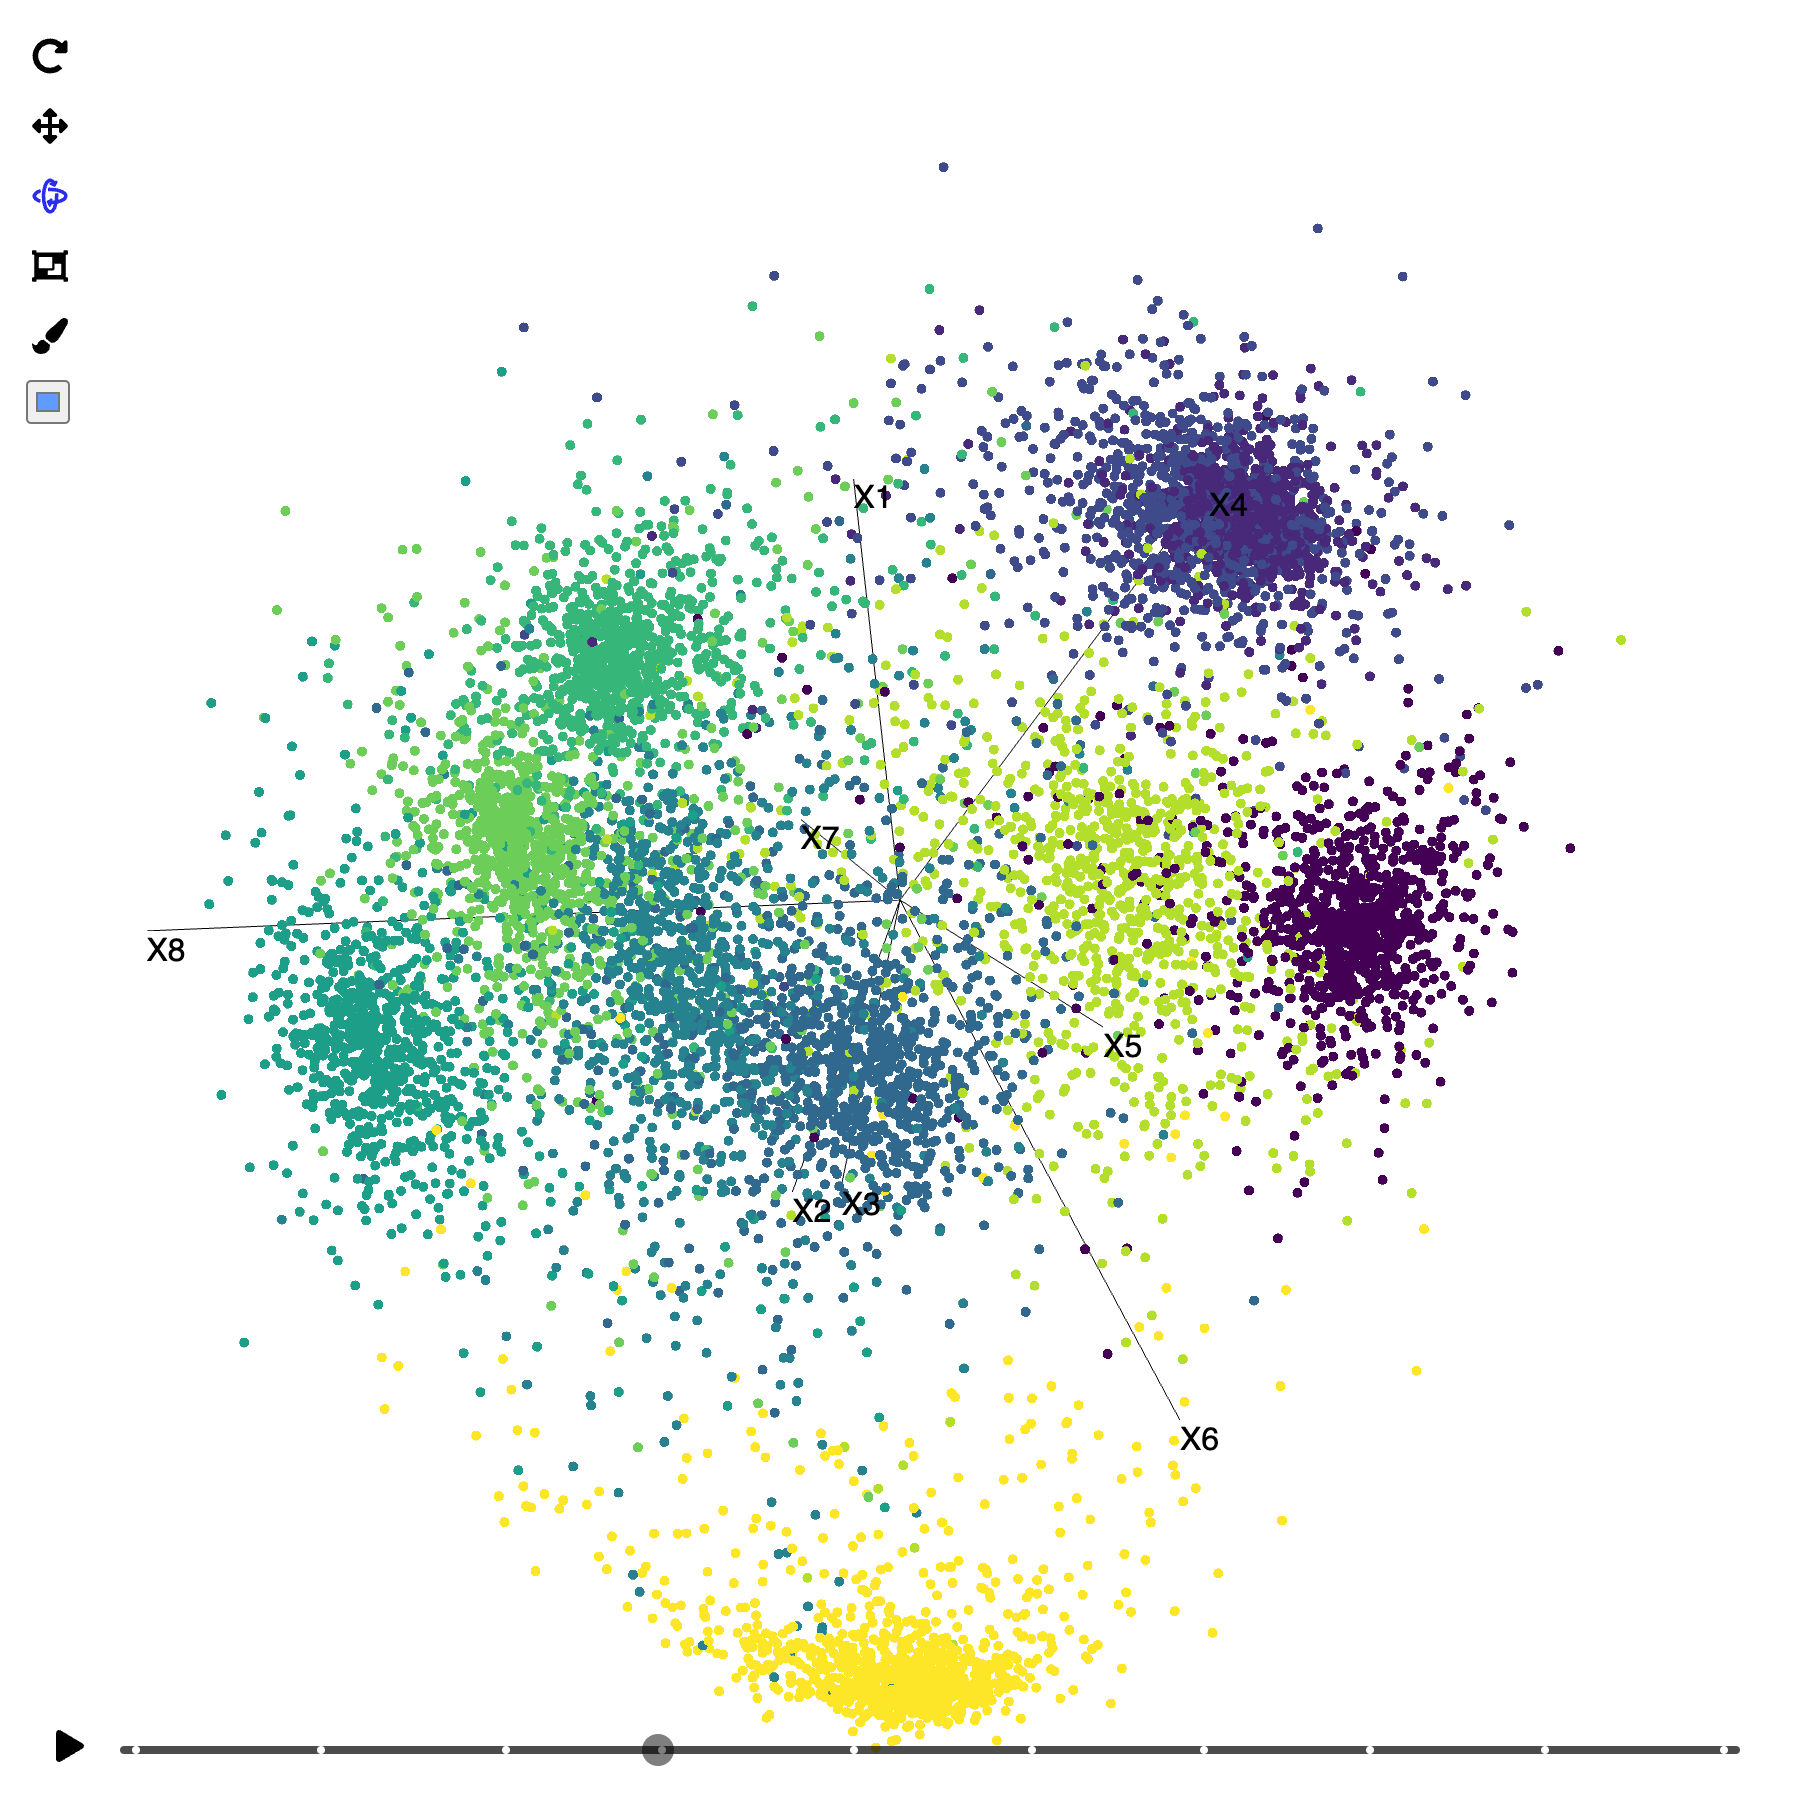
\includegraphics[width=0.49\linewidth]{figures/mnist/mnist-8d-scatter-2} 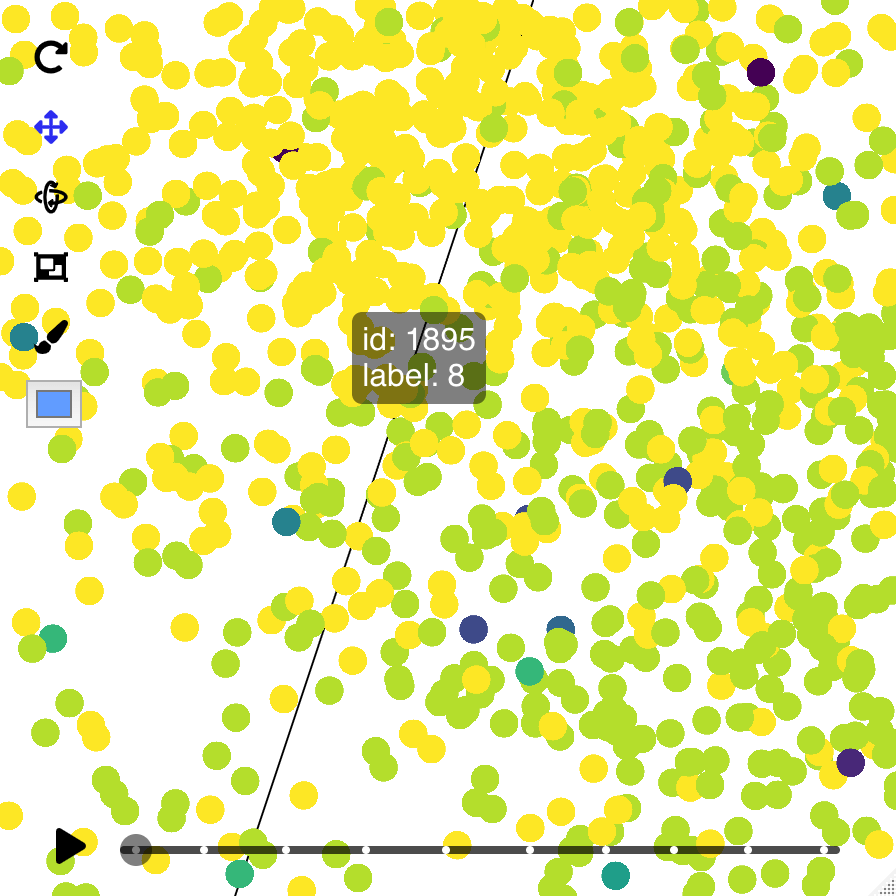
\includegraphics[width=0.49\linewidth]{figures/mnist/mnist-8d-scatter-label} 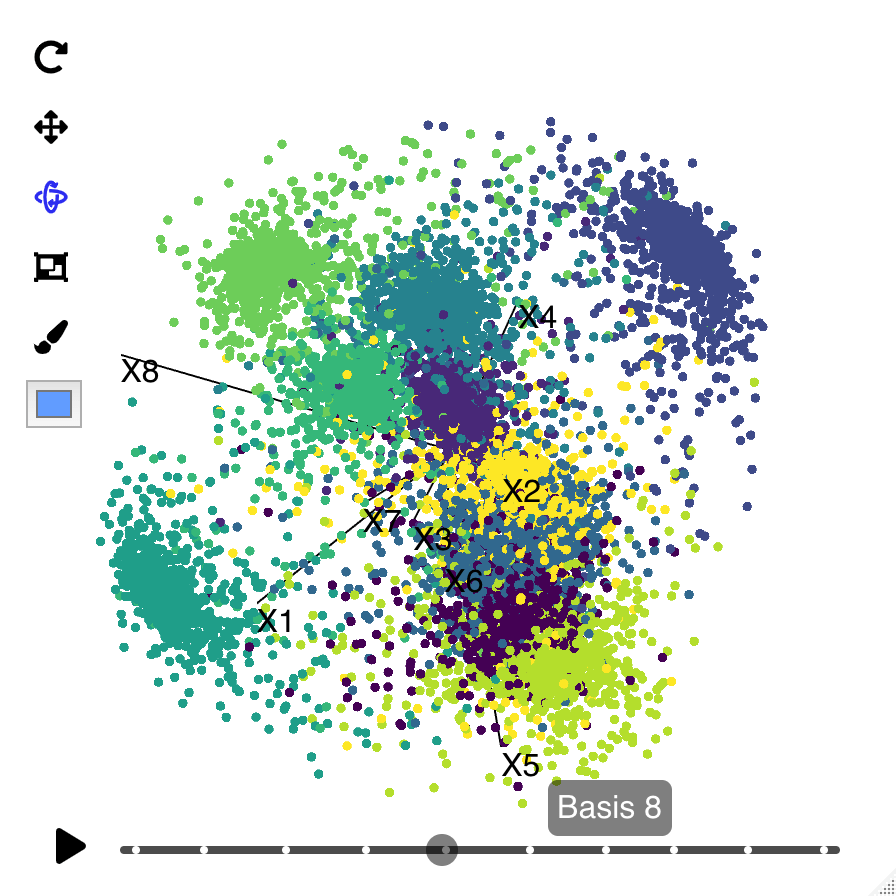
\includegraphics[width=0.49\linewidth]{figures/mnist/mnist-8d-scatter-timeline} 

}

\caption{Selected frames from the 8-dimensional MNIST embeddings data using show\_scatter() as the display method. The colour corresponds to the handwritten digit 0, 1, ..., 9. Despite the large number of data points, the animation of the tour is smooth and interactions are responsive.}\label{fig:mnist-8d-scatter}
\end{figure}

Using the core \texttt{show\_scatter()} function to display a \texttt{grand\_tour()} tour path in Figure \ref{fig:mnist-8d-scatter} we can see quite good separation between the clusters corresponding to each of the 10 digits. Despite the tour animation consisting of 10,000 data points, the animation runs smoothly at 30 FPS in Microsoft Edge on a Macbook Pro 2019. Running a performance profile of the animation indicates the CPU is idle 90\% of the time while the animation is playing. The remaining time is divided between scripting (6\%, including linear algebra operations), rendering (1.4\%), painting (0.8\%) and system (1.8\%). When running the same tour on the \texttt{mnist\_embeddings\_32d} dataset, the animation is still quite smooth and CPU is 80\% idle.

In the lower left of Figure \ref{fig:mnist-8d-scatter} is an example of the \texttt{label} aesthetic at work. This allows the user to identify which group a set of points belongs to, as well as the precise ID of any outliers that may require further investigation.

\hypertarget{sage-and-slice-display-methods}{%
\subsection{Sage and Slice display methods}\label{sage-and-slice-display-methods}}

\begin{figure}

{\centering 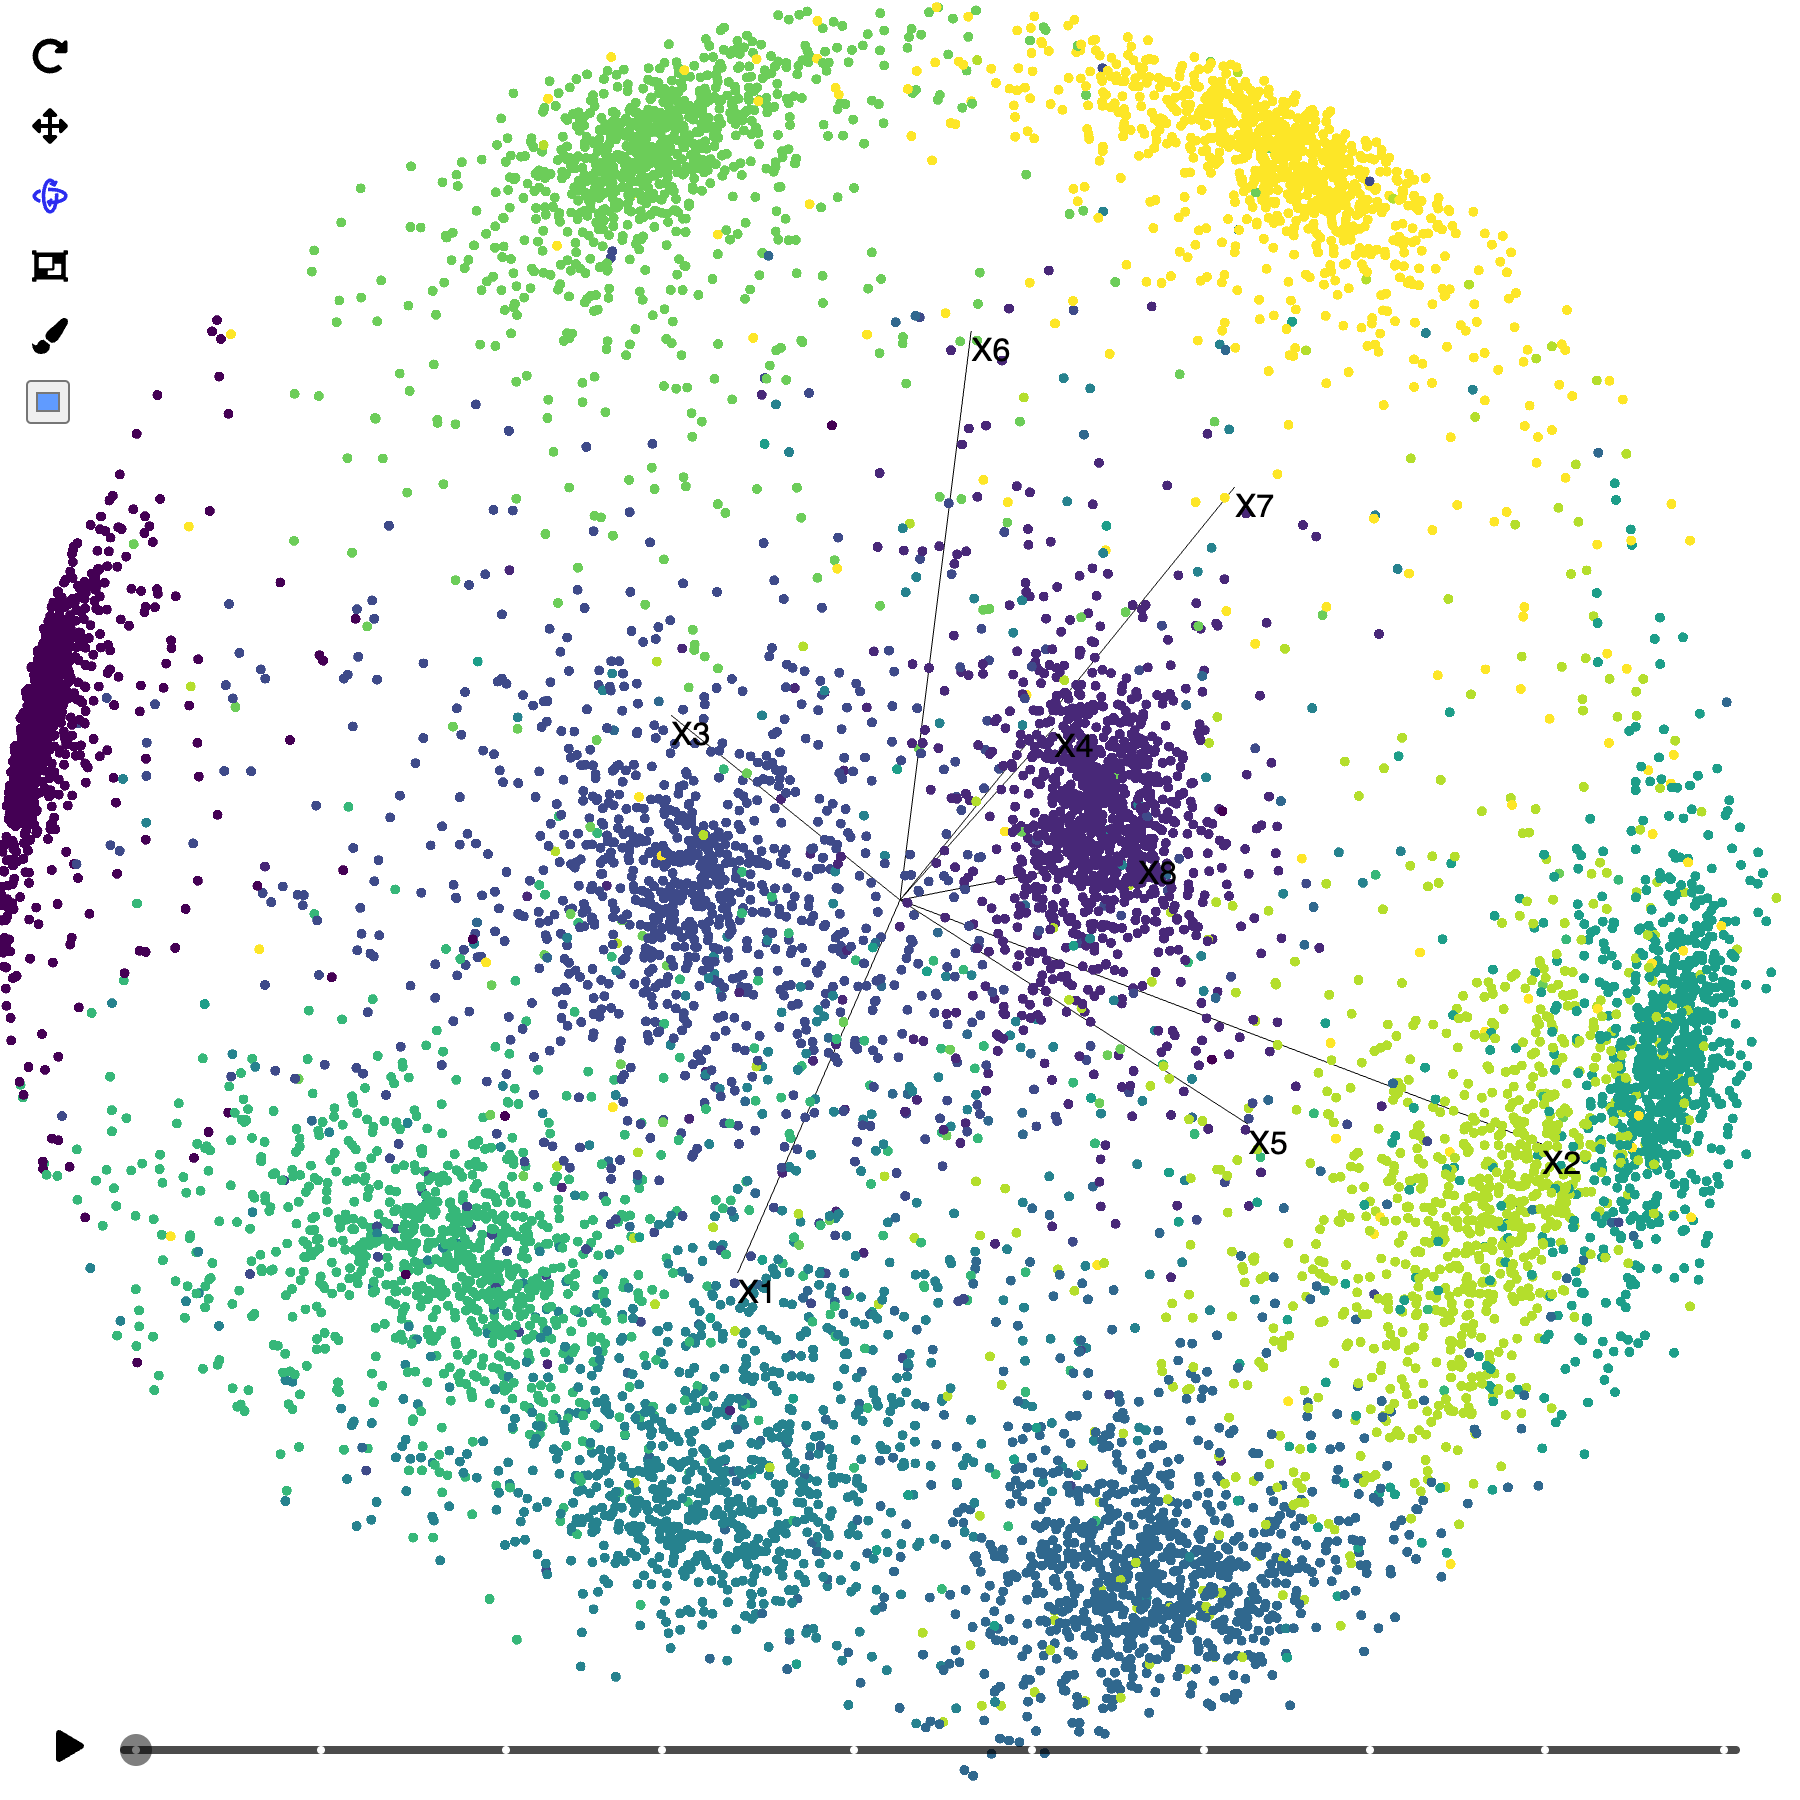
\includegraphics[width=0.49\linewidth]{figures/mnist/mnist-8d-sage-1} 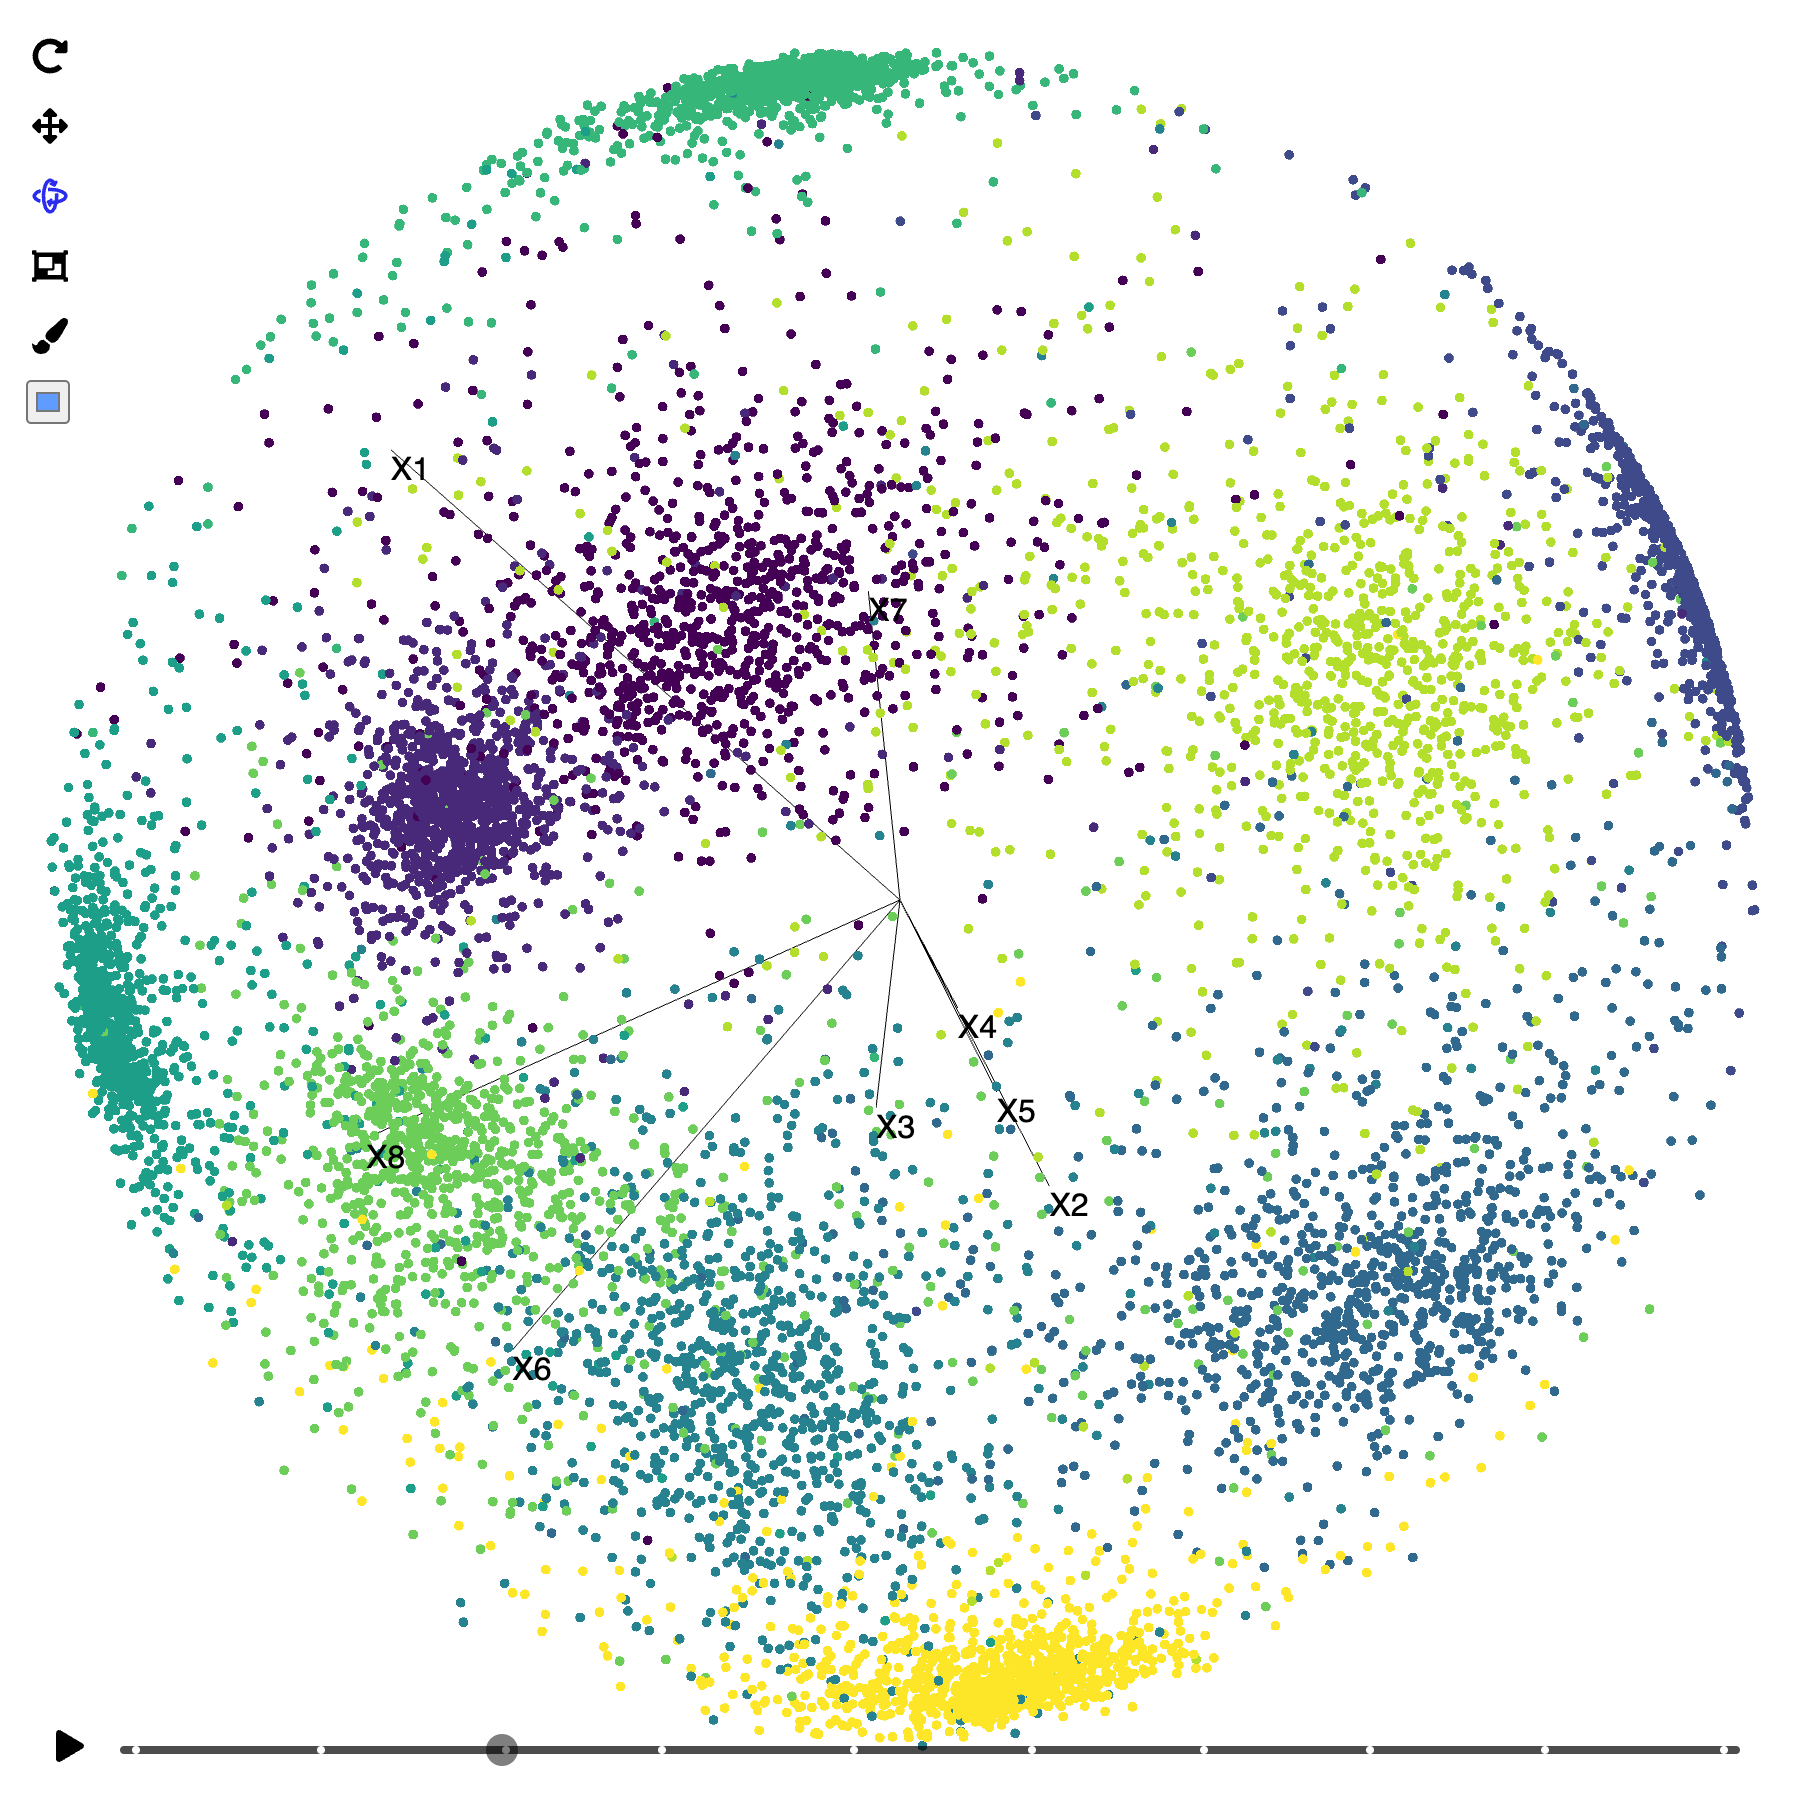
\includegraphics[width=0.49\linewidth]{figures/mnist/mnist-8d-sage-2} 

}

\caption{Selected frames from the 8-dimensional MNIST embeddings data using show\_sage() as the display method with a 2D grand tour path. The sage display shows the data points near the surface of the unit ball, which is due to the L2 normalisation of the original embeddings. This structure was not clear in the standard scatter display but is preserved with the sage display.}\label{fig:mnist-8d-sage}
\end{figure}

The \texttt{show\_scatter()} display method gives the viewer a fairly good sense of the data set, but there is some structure that may not be obvious. The embeddings in the \texttt{mnist\_embeddings\_8d} and \texttt{mnist\_embeddings\_32d} datasets are L2 normalised, so the points sit on the surface of a unit ball in the high-dimensional space. To reveal this structure, we can use the \emph{sage} (Laa, Cook, and Lee (2021)) or \emph{slice} (Laa, Cook, and Valencia (2020)) display methods, which are implemented as \texttt{show\_sage()} and \texttt{show\_slice()} respectively.

The \emph{sage} display scales points outwards based on their radius so that the relative volume of the circle or sphere in the projected space is the same as in the original space. In the example shown in Figure \ref{fig:mnist-8d-sage}, the \texttt{show\_sage()} display method is used. The effect is that the projected points tend sit much closer to the surface of the unit circle, giving a much clearer view of the ball-like structure of the original data.

\begin{figure}

{\centering 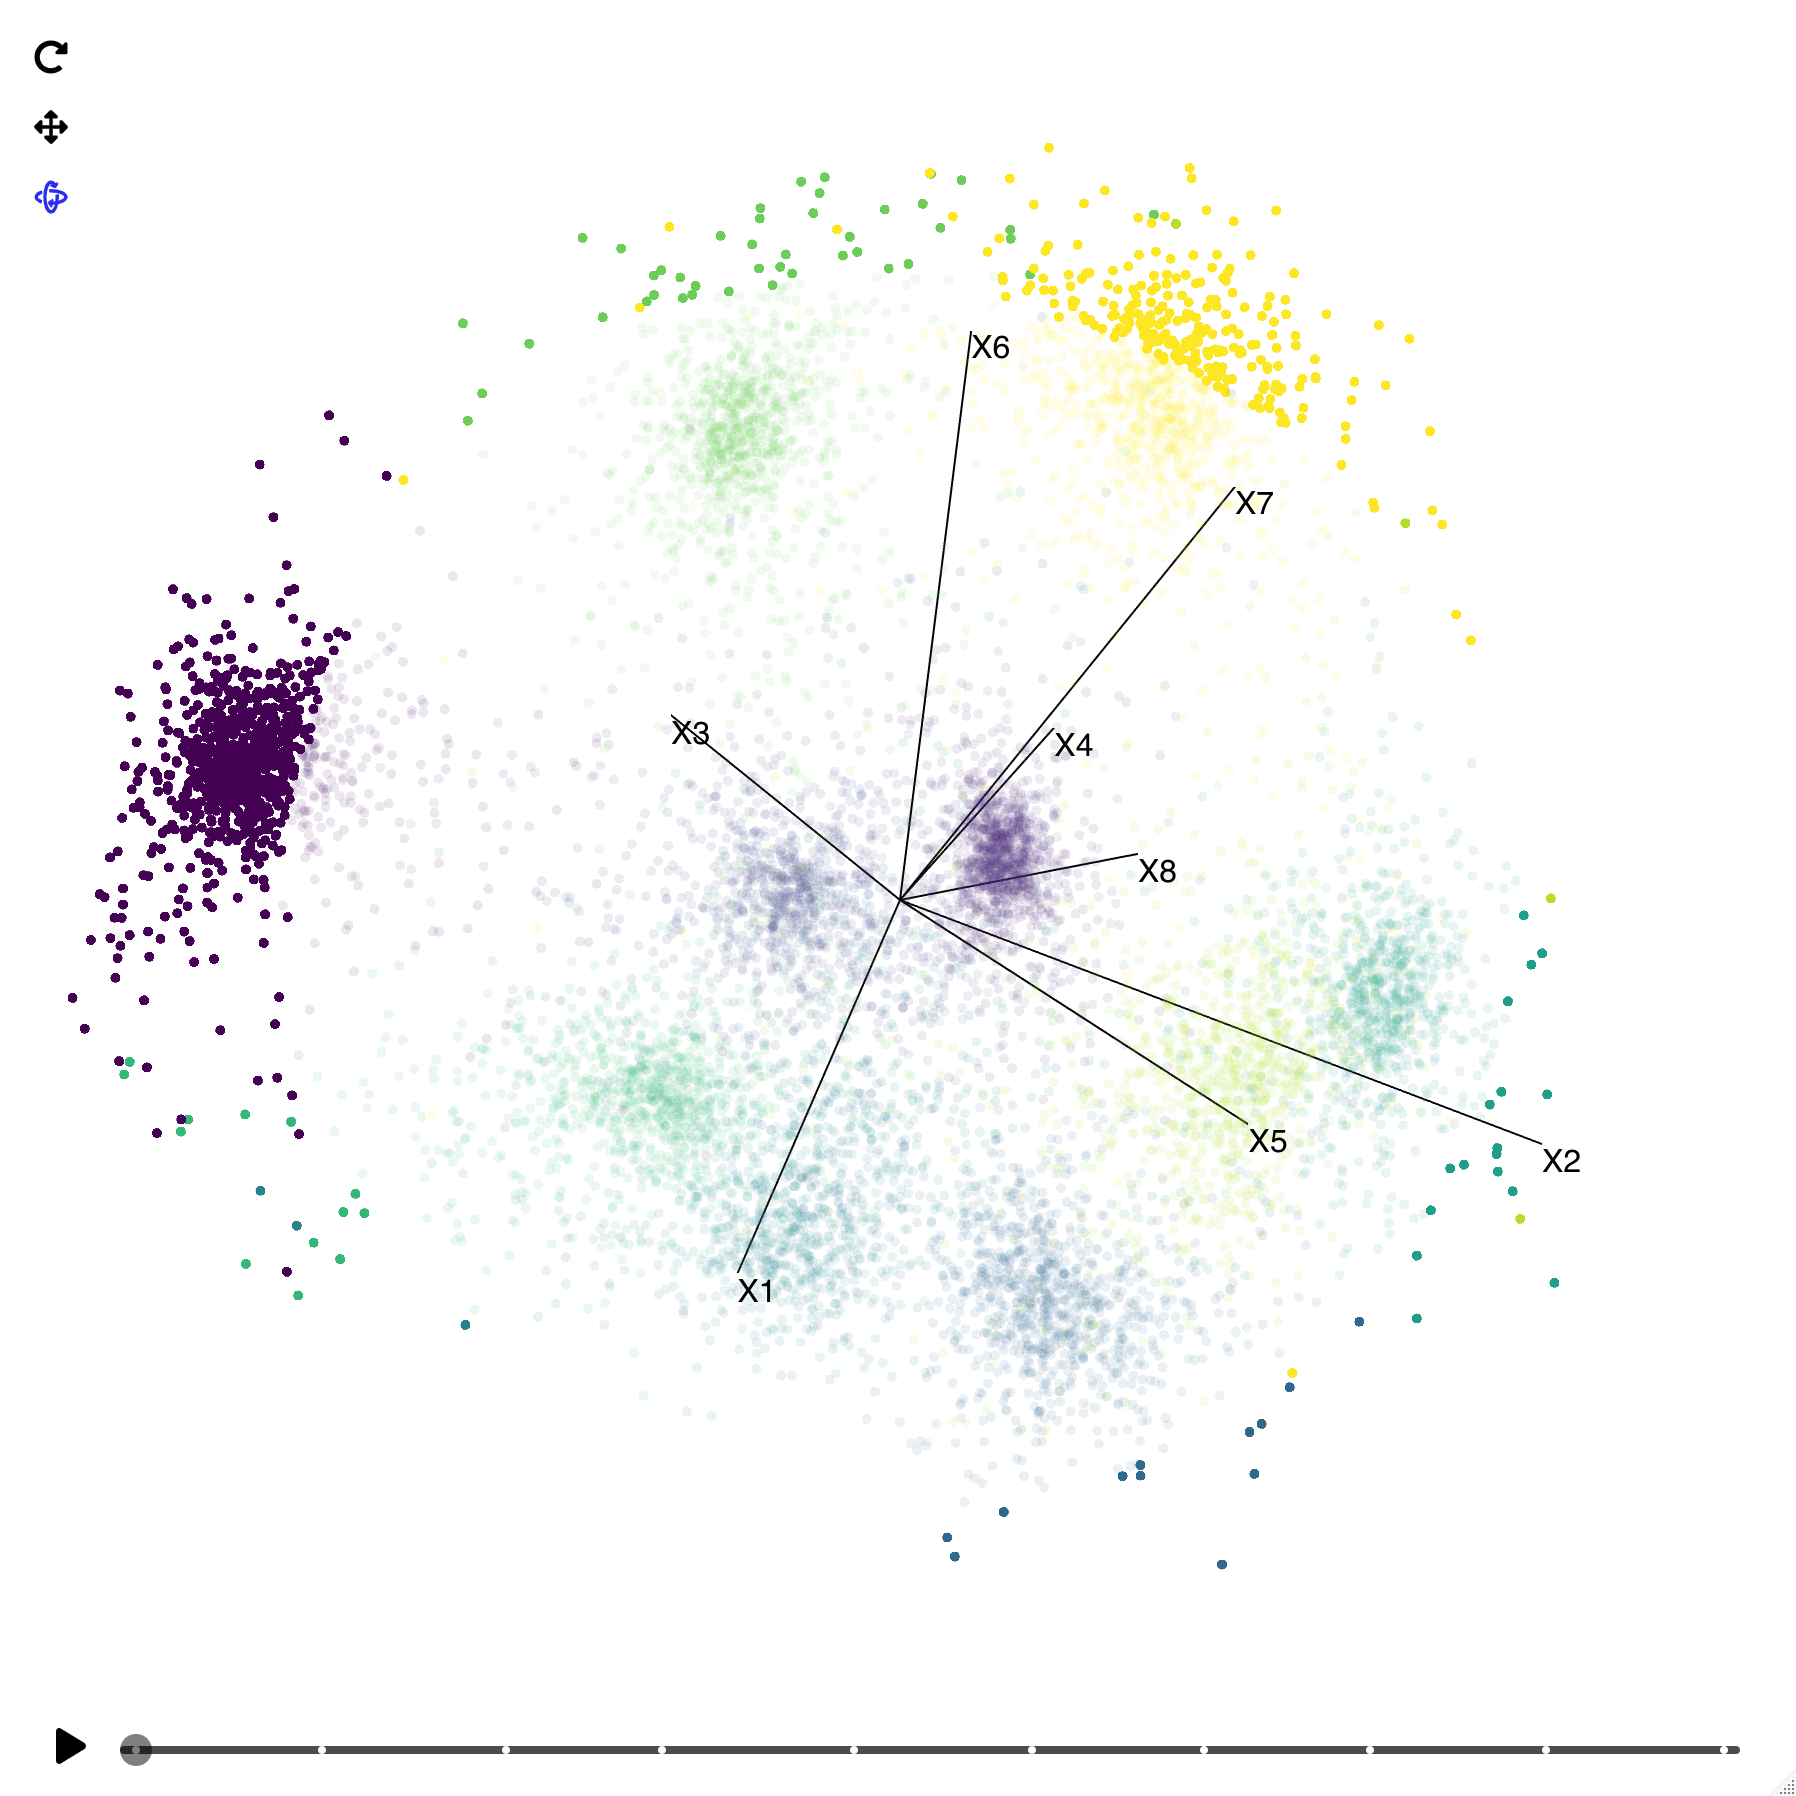
\includegraphics[width=0.49\linewidth]{figures/mnist/mnist-8d-slice-1} 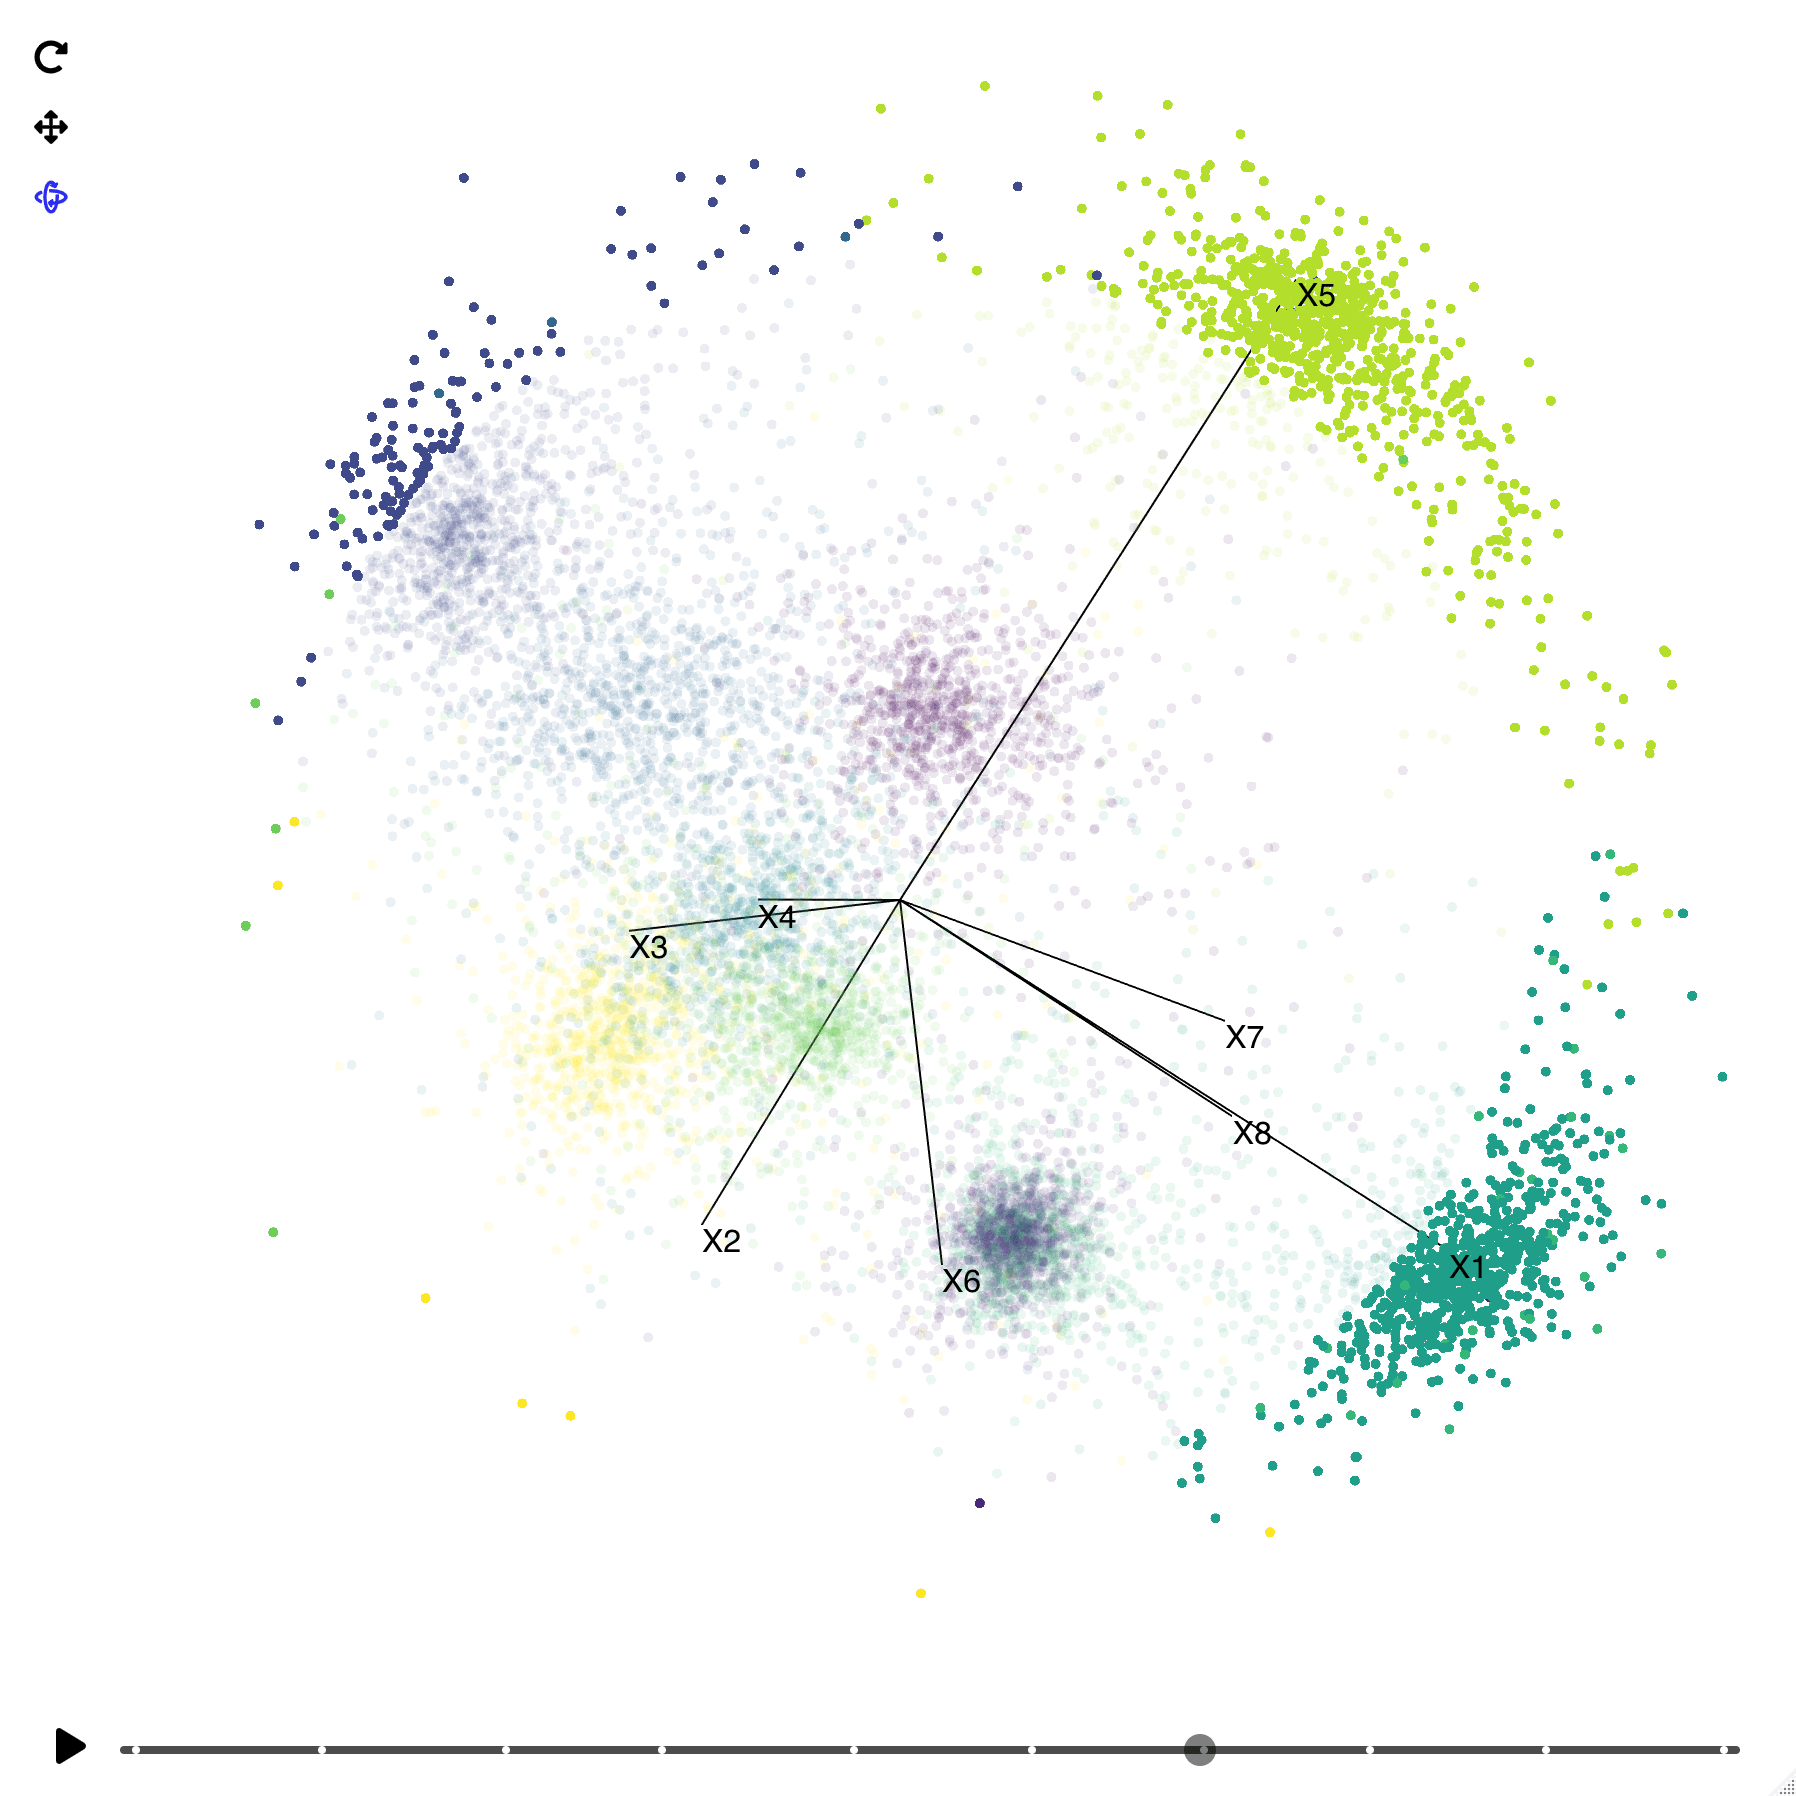
\includegraphics[width=0.49\linewidth]{figures/mnist/mnist-8d-slice-2} 

}

\caption{Selected frames of the 8-dimensional MNIST embeddings data using show\_slice() as the display method. The slice display makes the hollowness of this data apparent.}\label{fig:mnist-8d-slice}
\end{figure}

The \emph{slice} display highlights points based on their proximity to the projection plane. Points that are close to the projection plane are highlighted and those further away are faded out by making them transparent. In the case of the MNIST embedding data in Figure \ref{fig:mnist-8d-slice} the ball structure of the data manifests as a clear circular void in the middle of the plot, with points highlighted only towards the edges.

\hypertarget{linked-selection}{%
\subsection{Linked selection}\label{linked-selection}}

Plot interactions such as selection and filtering can be helpful for identifying and exploring outliers, clusters, and other interesting features in a dataset. These are enhanced even further when multiple visuals are linked, and selections and filters are applied to all linked visuals. In this example, we compare the tour animation with the result of a T-SNE (Van der Maaten and Hinton (2008)) which was performed using the excellent \CRANpkg{Rtsne} R package (Krijthe (2015)) and displayed using \pkg{plotly}. The visuals are linked using the R package \pkg{crosstalk} and a set of filter checkboxes is also added.

\begin{figure}
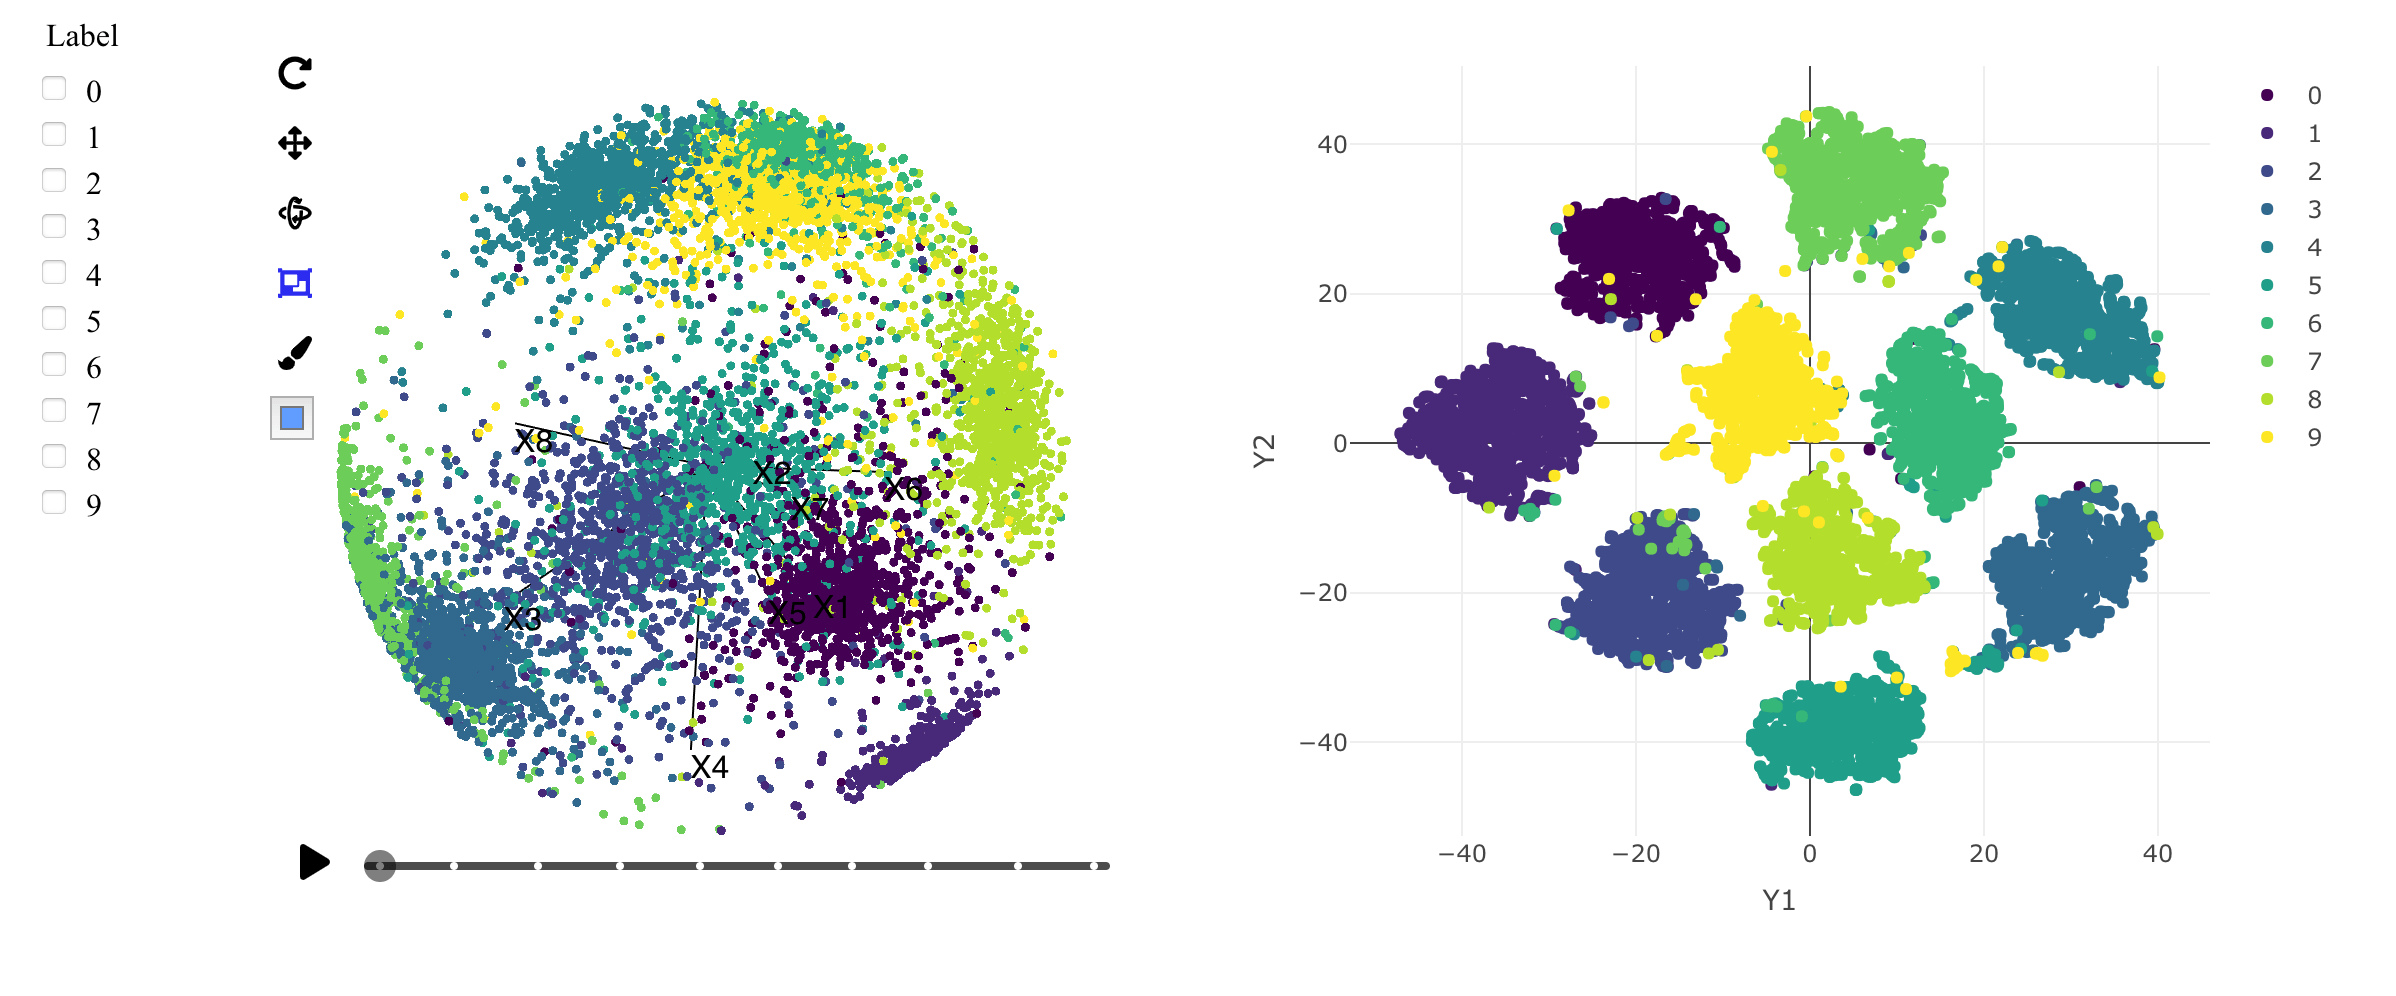
\includegraphics[width=\textwidth]{figures/mnist/case-study-linked-brushing-full} \caption{Linked visuals of the tour using detourr (left) compared to a T-SNE dimension reduction (right)}\label{fig:linked-tsne-full}
\end{figure}

Figure \ref{fig:linked-tsne-full} shows the linked visuals in their initial state with no filtering applied. We can then use the selection tool in either of the visuals to highlight points, and see the highlighting applied to both visuals as in Figure \ref{fig:linked-tsne-selection}.

\begin{figure}
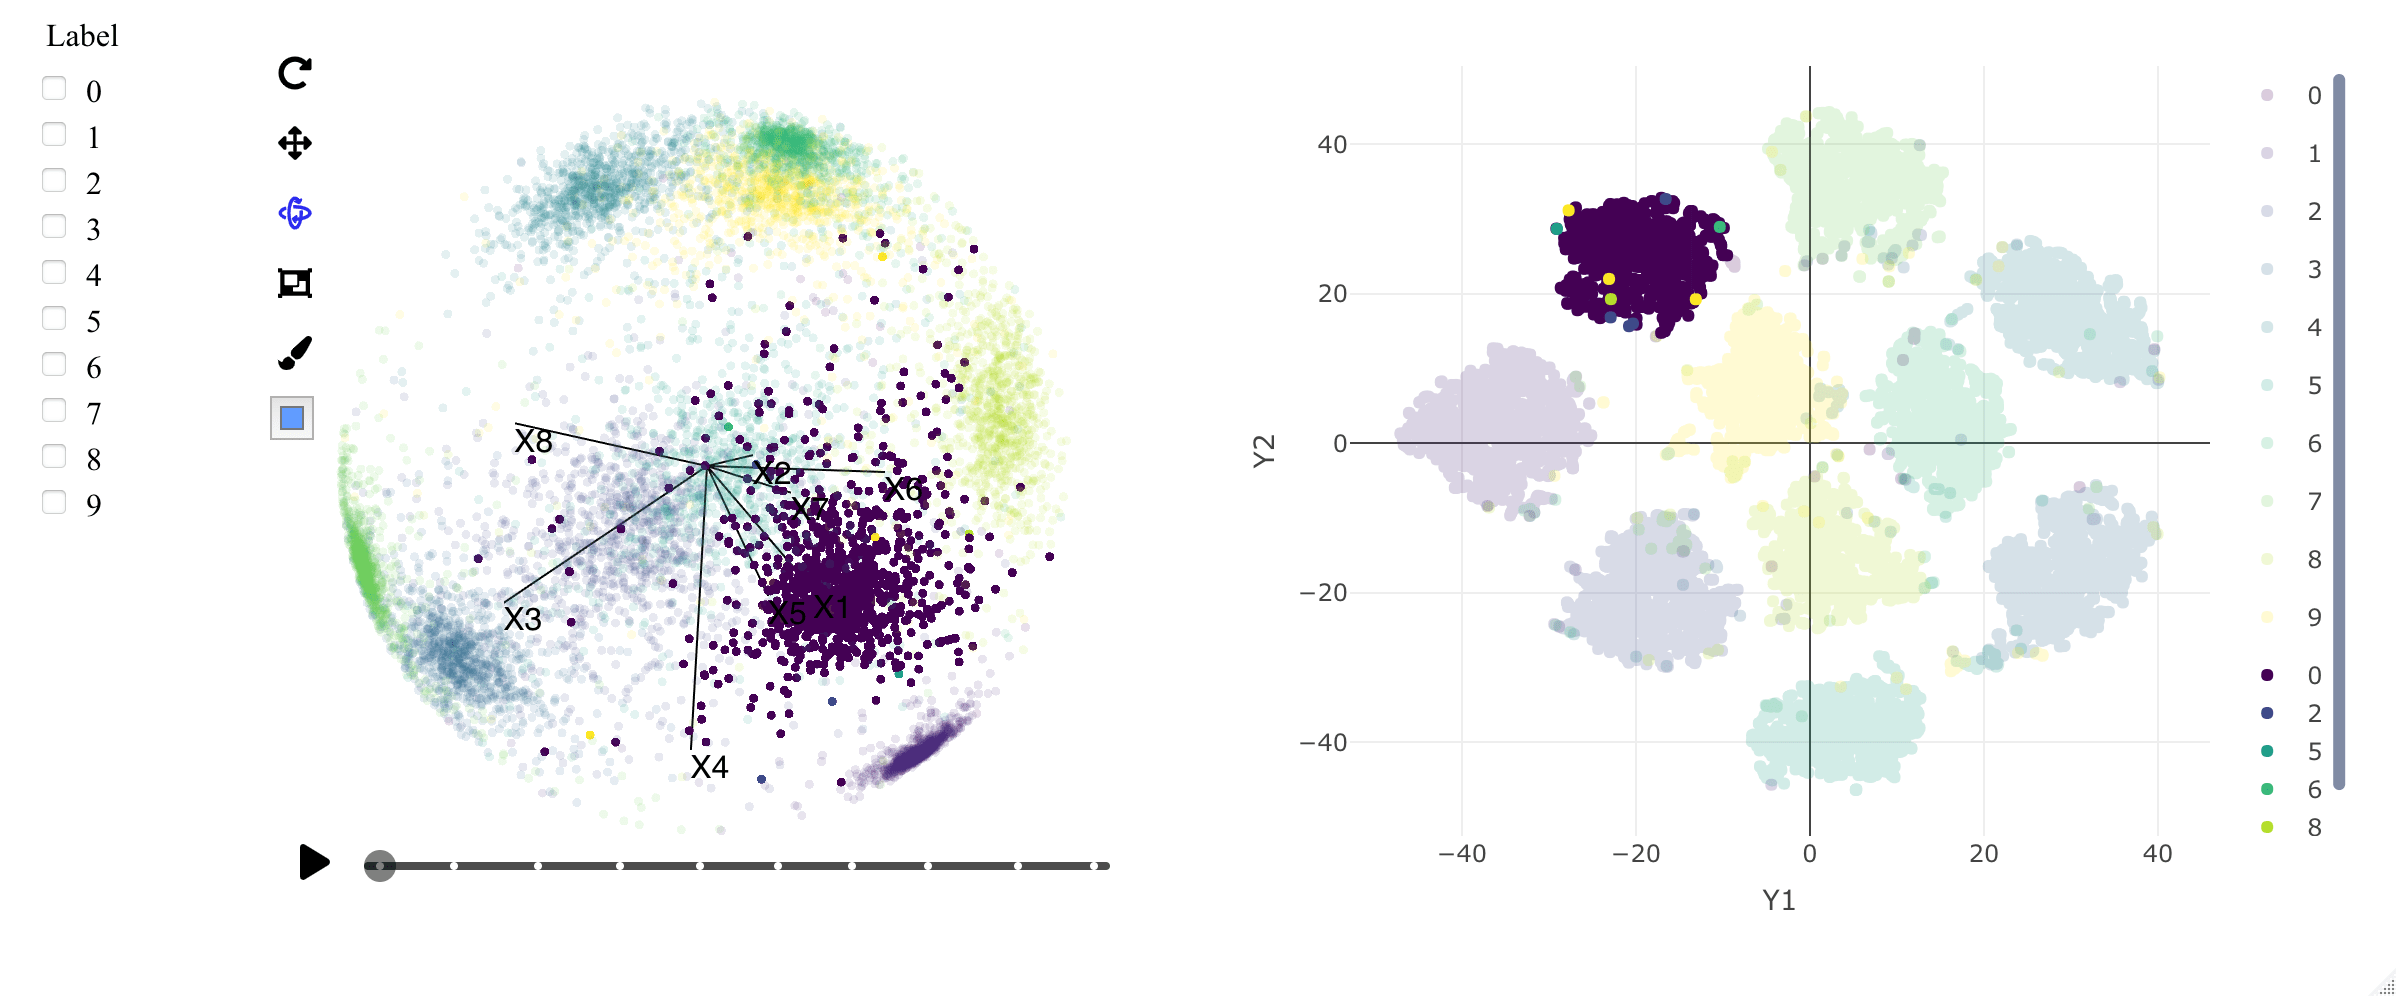
\includegraphics[width=\textwidth]{figures/mnist/case-study-linked-brushing-selection} \caption{Linked visuals with selection applied. Points can be selected in either visual via click-and-drag and the selection will be reflected in both.}\label{fig:linked-tsne-selection}
\end{figure}

Figure \ref{fig:linked-tsne-filter} shows the result of filtering the visuals using the filter checkboxes on the left. In the filtered visual, outlying points are much easier to see, and they can be easily investigated using tooltips.

\begin{figure}
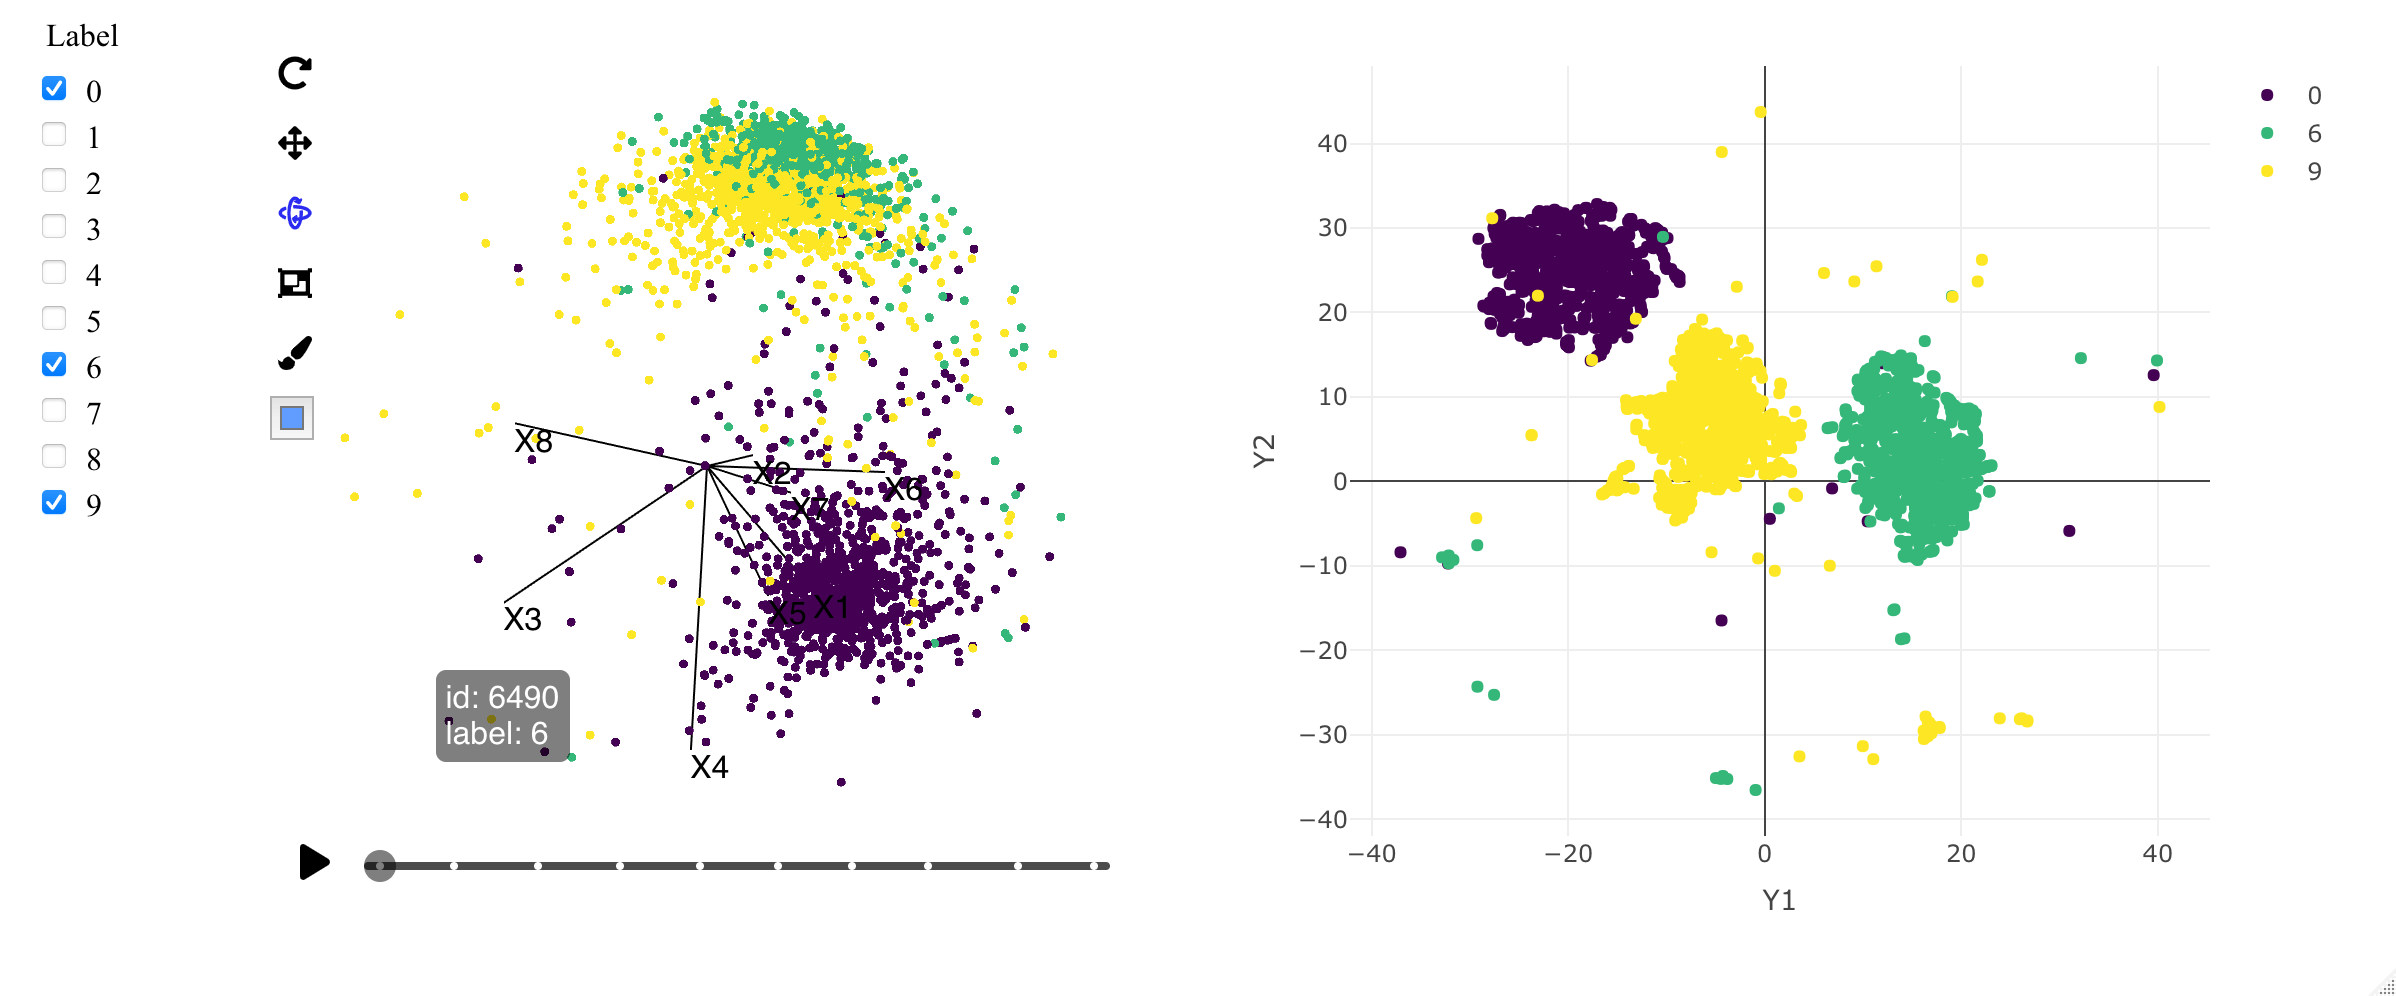
\includegraphics[width=\textwidth]{figures/mnist/case-study-linked-brushing-filter} \caption{Linked visuals with filtering applied. Viewing each digit individually makes outlying points much more apparent, and those points can be identified using tooltips.}\label{fig:linked-tsne-filter}
\end{figure}

\pagebreak

The code used to produce figures \ref{fig:linked-tsne-full}, \ref{fig:linked-tsne-selection}, and \ref{fig:linked-tsne-filter} is shown below. Here each plot is created using a \pkg{crosstalk} \texttt{SharedData} object in place of a standard data frame, and linked together using the \texttt{bscols} function:

\begin{verbatim}
library(crosstalk)
library(Rtsne)
library(plotly)

data(mnist_embeddings_8d)

ts <- select(mnist_embeddings_8d, starts_with("X")) |>
    Rtsne(num_threads = 4)
Y <- as_tibble(ts$Y)
names(Y) <- c("Y1", "Y2")

plot_df <- bind_cols(mnist_embeddings_8d, Y)
shared_mnist <- SharedData$new(plot_df)

detour_plot <- detour(shared_mnist, tour_aes(
    projection = starts_with("X"), color = label,
    label = c(id, label),
)) |>
    tour_path(grand_tour(2)) |>
    show_sage(width = "100%", height = "450px")

tsne_plot <- plot_ly(shared_mnist,
    x = ~Y1,
    y = ~Y2,
    text = paste0("Label: ", plot_df$label, "<br>", "ID: ", plot_df$id),
    color = ~label,
    height = 450,
    colors = viridisLite::viridis(10)
) |>
    highlight(on = "plotly_selected", off = "plotly_doubleclick") |>
    add_trace(type = "scatter", mode = "markers")

bscols(
    list(
        filter_checkbox("label", "Label", shared_mnist, ~label)
    ),
    detour_plot, tsne_plot,
    widths = c(1, 5, 6)
)
\end{verbatim}

\hypertarget{conclusion-and-future-work}{%
\section{Conclusion and future work}\label{conclusion-and-future-work}}

In this paper we have introduced \pkg{detourr} which provides interactive, performant, and portable tour visualisations from R. We accomplish these things using web technologies; TensorFlow.js (Abadi et al. (2016)) provides fast linear algebra operations through WebAssembly, Three.js provides GPU rendering via WebGL, and JavaScript \& HTML enable good performance and interactive features across the board. We also provide a simplified implementation of the Slice display (Laa, Cook, and Valencia (2020)), and have generalised the radial transformation from the Sage display (Laa, Cook, and Lee (2021)) to work with tours of 3 or more dimensions. All of this is done with an intuitive user interface which makes the software accessible to new users.

Looking ahead, the priority for the next stage of development is to leverage \pkg{detourr}'s extensible design to implement additional display methods such as density plots, histograms, parallel coordinates plots, and Andrew's plot. Additional changes could also be made to allow the radial transformation of the sage display and the highlighting of points from the slice display to be incorporated in to these other display methods, rather than being limited to only the scatter plot display. This would also allow the additional information from both the sage and slice tour applied to the same visual.

Further enhancements could be made by implementing facetting; allowing grouped data to be displayed across separate visuals with unified controls and timeline added. This could be taken further by allowing multiple \emph{different} displays to use the same controls and timeline, for example displaying a scatter plot alongside one or more density plots.

To extend the existing scatter plot displays, the addition of an interactive legend would greatly enhance the user experience. As well as providing context for the point colour / fill, this would allow the user to be able to filter groups without needing to use a separate package like \pkg{shiny} or \pkg{crosstalk}. A shape aesthetic would also be beneficial, and the ability to export the projection matrix at the current frame would make it easier to perform analysis once an interesting projection is found.

As well as being able to display points and lines, support for plotting surfaces would allow for rich visualisations of regression model fits and classification boundaries. Three.js has good support for drawing surfaces, however it's not clear how a decision boundary can be projected down to a lower number of dimensions or whether this is actually feasible.

Support for displaying images or sprites directly on the tour visual or as an extension of the tooltip functionality is possible. A similar feature is implemented in the Tensorboard Embedding Visualiser (Smilkov et al. (2016)) which also uses Three.js under the hood.

What's more, Three.js has support for VR, which would be an interesting addition for exploring an immersive 3D tour visual.

\pagebreak

\hypertarget{radial-cdf-of-hyperspheres-projected-to-3-dimensions}{%
\section{Radial CDF of hyperspheres projected to 3 dimensions}\label{radial-cdf-of-hyperspheres-projected-to-3-dimensions}}

In order to implement the 3D variant of the sage tour (Laa, Cook, and Lee (2021)), we need an expression for the relative projected volume of a \textbf{sphere} of radius \(R\). This is then used as a scaling factor for point radii in the visualisation to prevent points from being crowded towards the centre.

First we denote the volume of a \(p\)-dimensional hypersphere by:

\[
\frac{2\pi^{p/2}R^p}{p\Gamma(p/2)}
\]

In the appendix of Laa et al. (2022) (equations 7--10) is a derivation for the relative projected volume of a ball of radius \(r\).

\begin{align}
    F(r; p, R) &= \frac{V_{inside}(r; p, R)}{ V(p, r) } \\
    &= 1 - \frac{V_{outside}(r; p, R)}{ V(p, r) }
    \label{eq:F2}
\end{align}

And the formula for \(V_{outside}(r; p, R)\) for a \textbf{circle} is given as:

\begin{equation}
V_{outside}(r; p, R) =
\int_r^R V(p-2, \sqrt{R^2 - x^2})2\pi x dx 
\label{eq:v-outside}
\end{equation}

To extend this to the 3-dimensional case, we can modify \eqref{eq:v-outside} to express the volume outside a \textbf{sphere} of radius \(r\) as:

\begin{equation}
  V_{outside}(r; p, R) = \int_r^R V(p-3, \sqrt{R^2 - x^2})4\pi x^2 dx
\end{equation}

and it follows that the relative projected volume for a sphere is

\begin{equation}
  F_3(r; p, R) = 1 - 
  \frac{
      \int_r^R V(p-3, \sqrt{R^2 - x^2})4\pi x^2 dx
  }{
      V(p, R)
  } 
\end{equation}

We know \(2\Gamma(3/2) = \Gamma(1/2) = \sqrt{ \pi }\) so with some rearranging this can be reduced to:

\begin{equation}
  F_3(r; p, R) = 1 - \frac{2}{R^p} \frac{\Gamma(p/2+1)}{\Gamma(3/2)\Gamma((p-1)/2)}
  \int_r^R (R^2 - x^2)^{(p-3)/2} x^2 dx \\
\end{equation}

Denoting \(u = 1 - \left(\frac{x}{R}\right)^2\) and \(dx = \frac{R^2}{-2x}du = \frac{R}{-2\sqrt{1-u}}du\) for a change of variable this becomes

\begin{align}
  F_3(r; p, R) &= 1 - \frac{\Gamma(p/2+1)}{\Gamma(3/2)\Gamma((p-1)/2)}
  \int_0^{1-\frac{r^2}{R^2}} u^{(p-3)/2} (1-u)^{1/2} du \\
  &= 1 - \mathrm{BetaInc}\left(1-\left(\frac{r}{R}\right)^2, \frac{p-1}{2}, \frac{3}{2}\right) \\
  &= \mathrm{BetaInc}\left(\left(\frac{r}{R}\right)^2, \frac{3}{2}, \frac{p-1}{2}\right) 
  \label{eq:betainc1}
\end{align}

where \emph{BetaInc} is the regularised incomplete beta function (the CDF of a Beta distribution).

We can generalise this to any projection from \(p\) to \(d\) dimensions using the same steps, but with

\begin{equation}
  V_{outside}(r; p, R, d) = \int_r^R V(p-d, \sqrt{R^2 - x^2}) 
  \frac{2\pi^{d/2}}{\Gamma(d/2)} x^{d-1} dx
\end{equation}

where \(\frac{2\pi^{d/2}}{\Gamma(d/2)} x^{d-1}\) is the surface area of a d-ball.

This results in the relative projected volume of a projection from \(p\) to \(d\) dimensions being given by:

\begin{equation}
F(r; p, R, d) = \mathrm{BetaInc}\left(\left(\frac{r}{R}\right)^2, \frac{d}{2}, \frac{p-d}{2}+1\right)
\label{eq:betainc2}
\end{equation}

Figures \ref{fig:radial-cdf-p} and \ref{fig:radial-cdf-d} compare the theoretical results from equations \eqref{eq:betainc1} and \eqref{eq:betainc2} respectively with simulated values.

\begin{figure}

{\centering 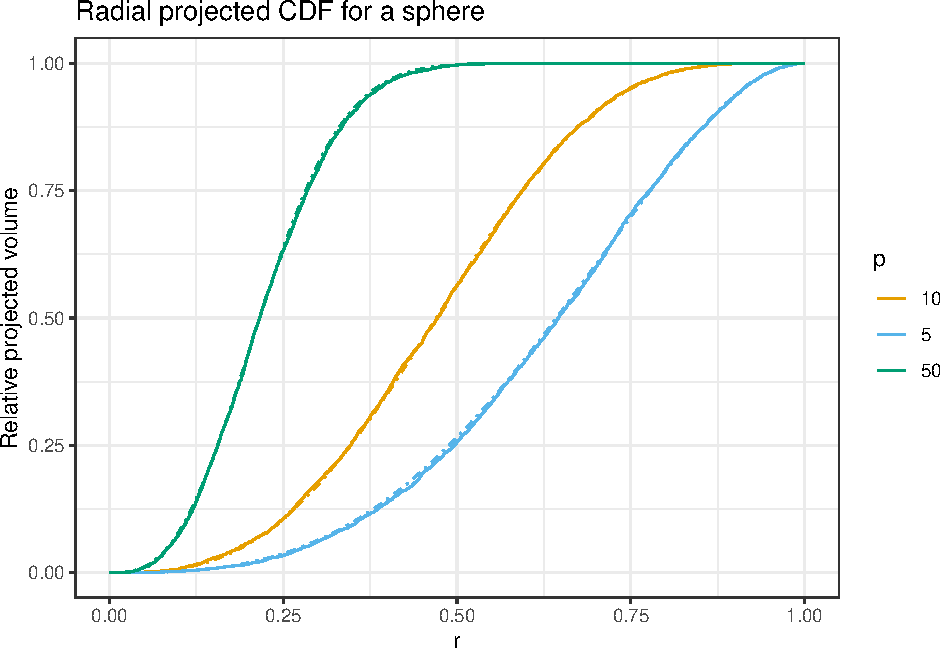
\includegraphics[width=0.75\linewidth]{RJ-2023-052_files/figure-latex/radial-cdf-p-1} 

}

\caption{Relative projected volume for projections from p dimensions to d=3 dimensions. The solid line is simulated data, and the dashed line is the theoretical CDF}\label{fig:radial-cdf-p}
\end{figure}

\begin{figure}

{\centering 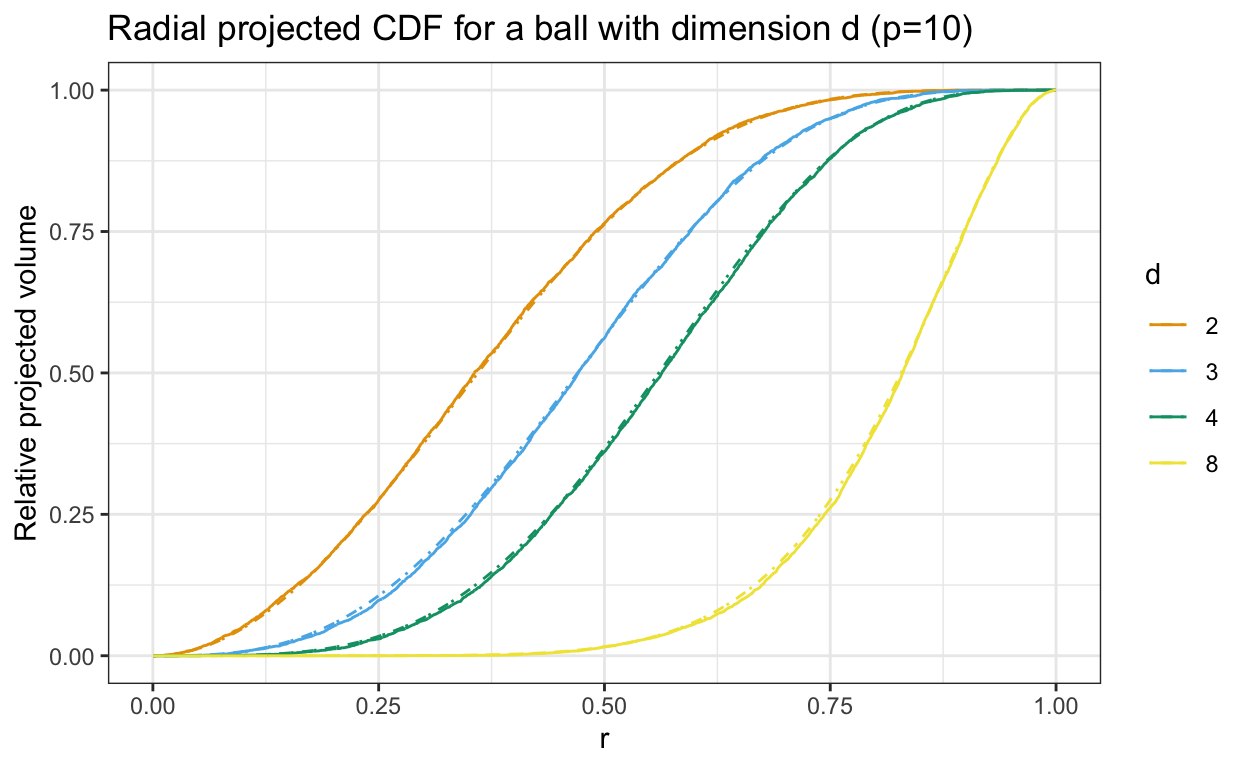
\includegraphics[width=0.75\linewidth]{RJ-2023-052_files/figure-latex/radial-cdf-d-1} 

}

\caption{Relative projected volume for a projection of p=10 dimensions to d dimensions.  The solid line is simulated data, and the dashed line is the theoretical CDF. This shows the generalisation to d > 3 dimensions}\label{fig:radial-cdf-d}
\end{figure}

\hypertarget{references}{%
\section*{References}\label{references}}
\addcontentsline{toc}{section}{References}

\hypertarget{refs}{}
\begin{CSLReferences}{1}{0}
\leavevmode\vadjust pre{\hypertarget{ref-abadi2016tensorflow}{}}%
Abadi, Martín, Paul Barham, Jianmin Chen, Zhifeng Chen, Andy Davis, Jeffrey Dean, Matthieu Devin, et al. 2016. {``TensorFlow: A System for Large-Scale Machine Learning.''} In \emph{12th USENIX Symposium on Operating Systems Design and Implementation (OSDI 16)}, 265--83.

\leavevmode\vadjust pre{\hypertarget{ref-rmarkdown}{}}%
Allaire, JJ, Yihui Xie, Jonathan McPherson, Javier Luraschi, Kevin Ushey, Aron Atkins, Hadley Wickham, Joe Cheng, Winston Chang, and Richard Iannone. 2022. \emph{Rmarkdown: Dynamic Documents for r}. \url{https://github.com/rstudio/rmarkdown}.

\leavevmode\vadjust pre{\hypertarget{ref-andrews1972plots}{}}%
Andrews, David F. 1972. {``Plots of High-Dimensional Data.''} \emph{Biometrics}, 125--36.

\leavevmode\vadjust pre{\hypertarget{ref-asimov1985grand}{}}%
Asimov, Daniel. 1985. {``The Grand Tour: A Tool for Viewing Multidimensional Data.''} \emph{SIAM Journal on Scientific and Statistical Computing} 6 (1): 128--43.

\leavevmode\vadjust pre{\hypertarget{ref-becker1987brushing}{}}%
Becker, Richard A, and William S Cleveland. 1987. {``Brushing Scatterplots.''} \emph{Technometrics} 29 (2): 127--42.

\leavevmode\vadjust pre{\hypertarget{ref-bostock2011d3}{}}%
Bostock, Michael, Vadim Ogievetsky, and Jeffrey Heer. 2011. {``D\(^3\) Data-Driven Documents.''} \emph{IEEE Transactions on Visualization and Computer Graphics} 17 (12): 2301--9.

\leavevmode\vadjust pre{\hypertarget{ref-buja2005computational}{}}%
Buja, Andreas, Dianne Cook, Daniel Asimov, and Catherine Hurley. 2005. {``Computational Methods for High-Dimensional Rotations in Data Visualization.''} \emph{Handbook of Statistics} 24: 391--413.

\leavevmode\vadjust pre{\hypertarget{ref-threejs}{}}%
Cabello, Ricardo. 2010. {``Three.js.''} \emph{GitHub Repository}. \url{https://github.com/mrdoob/three.js}.

\leavevmode\vadjust pre{\hypertarget{ref-shiny}{}}%
Chang, Winston, Joe Cheng, JJ Allaire, Carson Sievert, Barret Schloerke, Yihui Xie, Jeff Allen, Jonathan McPherson, Alan Dipert, and Barbara Borges. 2021. \emph{Shiny: Web Application Framework for r}. \url{\%7Bhttps://CRAN.R-project.org/package=shiny\%7D}.

\leavevmode\vadjust pre{\hypertarget{ref-leaflet}{}}%
Cheng, Joe, Bhaskar Karambelkar, and Yihui Xie. 2022. \emph{Leaflet: Create Interactive Web Maps with the JavaScript 'Leaflet' Library}. \url{\%7Bhttps://CRAN.R-project.org/package=leaflet\%7D}.

\leavevmode\vadjust pre{\hypertarget{ref-crosstalk}{}}%
Cheng, Joe, and Carson Sievert. 2022. \emph{Crosstalk: Inter-Widget Interactivity for HTML Widgets}. \url{\%7Bhttps://rstudio.github.io/crosstalk/\%7D}.

\leavevmode\vadjust pre{\hypertarget{ref-cook2007interactive}{}}%
Cook, Dianne, Deborah F Swayne, and Andreas Buja. 2007. \emph{Interactive and Dynamic Graphics for Data Analysis: With r and GGobi}. Springer Science \& Business Media.

\leavevmode\vadjust pre{\hypertarget{ref-harrison2022langevitour}{}}%
Harrison, Paul. 2022. \emph{Langevitour: Langevin Tour}. \url{\%7Bhttps://CRAN.R-project.org/package=langevitour\%7D}.

\leavevmode\vadjust pre{\hypertarget{ref-hastie2009elements}{}}%
Hastie, Trevor, Robert Tibshirani, Jerome H Friedman, and Jerome H Friedman. 2001. \emph{The Elements of Statistical Learning: Data Mining, Inference, and Prediction}. Springer.

\leavevmode\vadjust pre{\hypertarget{ref-tidyselect}{}}%
Henry, Lionel, and Hadley Wickham. 2022. \emph{Tidyselect: Select from a Set of Strings}. \url{\%7Bhttps://CRAN.R-project.org/package=tidyselect\%7D}.

\leavevmode\vadjust pre{\hypertarget{ref-kipp2019connecting}{}}%
Kipp, Michael, Ursula Laa, and Dianne Cook. 2019. {``Connecting r with D3 for Dynamic Graphics, to Explore Multivariate Data with Tours.''} \emph{The R Journal} 11 (1): 245.

\leavevmode\vadjust pre{\hypertarget{ref-van2015rtsne}{}}%
Krijthe, Jesse H. 2015. \emph{{Rtsne}: T-Distributed Stochastic Neighbor Embedding Using Barnes-Hut Implementation}. \url{https://github.com/jkrijthe/Rtsne}.

\leavevmode\vadjust pre{\hypertarget{ref-laa2020hole}{}}%
Laa, Ursula, Dianne Cook, Andreas Buja, and German Valencia. 2022. {``Hole or Grain? A Section Pursuit Index for Finding Hidden Structure in Multiple Dimensions.''} \emph{Journal of Computational and Graphical Statistics} 0 (0): 1--14. \url{https://doi.org/10.1080/10618600.2022.2035230}.

\leavevmode\vadjust pre{\hypertarget{ref-laa2021burning}{}}%
Laa, Ursula, Dianne Cook, and Stuart Lee. 2021. {``Burning Sage: Reversing the Curse of Dimensionality in the Visualization of High-Dimensional Data.''} \emph{Journal of Computational and Graphical Statistics}, 1--10.

\leavevmode\vadjust pre{\hypertarget{ref-laa2020slice}{}}%
Laa, Ursula, Dianne Cook, and German Valencia. 2020. {``A Slice Tour for Finding Hollowness in High-Dimensional Data.''} \emph{Journal of Computational and Graphical Statistics} 29 (3): 681--87.

\leavevmode\vadjust pre{\hypertarget{ref-lecun1998mnist}{}}%
LeCun, Yann. 1998. {``The MNIST Database of Handwritten Digits.''} \emph{Http://Yann. Lecun. Com/Exdb/Mnist/}.

\leavevmode\vadjust pre{\hypertarget{ref-lee2021liminal}{}}%
Lee, Stuart. 2021. \emph{Liminal: Multivariate Data Visualization with Tours and Embeddings}. \url{\%7Bhttps://CRAN.R-project.org/package=liminal\%7D}.

\leavevmode\vadjust pre{\hypertarget{ref-mcinnes2018umap}{}}%
McInnes, Leland, John Healy, and James Melville. 2018. {``UMAP: Uniform Manifold Approximation and Projection for Dimension Reduction.''} arXiv. \url{https://doi.org/10.48550/ARXIV.1802.03426}.

\leavevmode\vadjust pre{\hypertarget{ref-gifski}{}}%
Ooms, Jeroen. 2021. \emph{Gifski: Highest Quality GIF Encoder}. \url{\%7Bhttps://CRAN.R-project.org/package=gifski\%7D}.

\leavevmode\vadjust pre{\hypertarget{ref-R}{}}%
R Core Team. 2021. \emph{R: A Language and Environment for Statistical Computing}. Vienna, Austria: R Foundation for Statistical Computing. \url{\%7Bhttps://www.R-project.org/\%7D}.

\leavevmode\vadjust pre{\hypertarget{ref-schroff2015facenet}{}}%
Schroff, Florian, Dmitry Kalenichenko, and James Philbin. 2015. {``Facenet: A Unified Embedding for Face Recognition and Clustering.''} In \emph{Proceedings of the IEEE Conference on Computer Vision and Pattern Recognition}, 815--23.

\leavevmode\vadjust pre{\hypertarget{ref-plotly}{}}%
Sievert, Carson. 2020. \emph{Interactive Web-Based Data Visualization with r, Plotly, and Shiny}. Chapman; Hall/CRC. \url{\%7Bhttps://plotly-r.com\%7D}.

\leavevmode\vadjust pre{\hypertarget{ref-smilkov2016embedding}{}}%
Smilkov, Daniel, Nikhil Thorat, Charles Nicholson, Emily Reif, Fernanda B. Viégas, and Martin Wattenberg. 2016. {``Embedding Projector: Interactive Visualization and Interpretation of Embeddings.''} arXiv. \url{https://doi.org/10.48550/ARXIV.1611.05469}.

\leavevmode\vadjust pre{\hypertarget{ref-spinifex}{}}%
Spyrison, Nicholas, and Dianne Cook. 2020. {``{spinifex: An R Package for Creating a Manual Tour of Low- dimensional Projections of Multivariate Data}.''} \emph{{The R Journal}} 12 (1): 243--57. \url{https://doi.org/10.32614/RJ-2020-027}.

\leavevmode\vadjust pre{\hypertarget{ref-swayne2003ggobi}{}}%
Swayne, Deborah F, Duncan Temple Lang, Andreas Buja, and Dianne Cook. 2003. {``GGobi: Evolving from XGobi into an Extensible Framework for Interactive Data Visualization.''} \emph{Computational Statistics \& Data Analysis} 43 (4): 423--44.

\leavevmode\vadjust pre{\hypertarget{ref-htmlwidgets}{}}%
Vaidyanathan, Ramnath, Yihui Xie, JJ Allaire, Joe Cheng, Carson Sievert, and Kenton Russell. 2021. \emph{Htmlwidgets: HTML Widgets for r}. \url{\%7Bhttps://CRAN.R-project.org/package=htmlwidgets\%7D}.

\leavevmode\vadjust pre{\hypertarget{ref-van2008tsne}{}}%
Van der Maaten, Laurens, and Geoffrey Hinton. 2008. {``Visualizing Data Using t-SNE.''} \emph{Journal of Machine Learning Research} 9 (11).

\leavevmode\vadjust pre{\hypertarget{ref-wang2018mapping}{}}%
Wang, Bo-Ting, TJ Hobbs, Sean Doyle, Jun Gao, Tie-Jiun Hou, Pavel M Nadolsky, and Fredrick I Olness. 2018. {``Mapping the Sensitivity of Hadronic Experiments to Nucleon Structure.''} \emph{Physical Review D} 98 (9): 094030.

\leavevmode\vadjust pre{\hypertarget{ref-wickham2010layered}{}}%
Wickham, Hadley. 2010. {``A Layered Grammar of Graphics.''} \emph{Journal of Computational and Graphical Statistics} 19 (1): 3--28.

\leavevmode\vadjust pre{\hypertarget{ref-tidydata}{}}%
---------. 2014. {``Tidy Data.''} \emph{The Journal of Statistical Software} 59. \url{http://www.jstatsoft.org/v59/i10/}.

\leavevmode\vadjust pre{\hypertarget{ref-wickham2016ggplot2}{}}%
---------. 2016. \emph{Ggplot2: Elegant Graphics for Data Analysis}. springer.

\leavevmode\vadjust pre{\hypertarget{ref-wickham2011tourr}{}}%
Wickham, Hadley, Dianne Cook, Heike Hofmann, and Andreas Buja. 2011. {``Tourr: An r Package for Exploring Multivariate Data with Projections.''} \emph{Journal of Statistical Software} 40: 1--18.

\leavevmode\vadjust pre{\hypertarget{ref-wilkinson2012grammar}{}}%
Wilkinson, Leland. 2012. {``The Grammar of Graphics.''} In \emph{Handbook of Computational Statistics}, 375--414. Springer.

\leavevmode\vadjust pre{\hypertarget{ref-dt}{}}%
Xie, Yihui, Joe Cheng, and Xianying Tan. 2022. \emph{DT: A Wrapper of the JavaScript Library 'DataTables'}. \url{\%7Bhttps://CRAN.R-project.org/package=DT\%7D}.

\end{CSLReferences}


\address{%
Casper Hart\\
University of Auckland\\%
Department of Statistics\\
%
%
%
\href{mailto:casperhart93@gmail.com}{\nolinkurl{casperhart93@gmail.com}}%
}

\address{%
Earo Wang\\
The University of Auckland\\%
Department of Statistics\\
%
%
%
\href{mailto:earo.wang@gmail.com}{\nolinkurl{earo.wang@gmail.com}}%
}

\end{article}


\end{document}
